%%%%%%%%%%%%%%%%%%%%%%%%%%%%%%%%%%%%%%%%%%%%%%%%%%%%%%%%%%%%%%%%%%%%%%%%%%%%%%%%%%%
%%%  Filename: main.tex
%%%  ---
%%%  Template for Bachelor Thesis at DTETI UGM   		
%%%  Created using thesisdtetiugm.cls
%%%  --- 
%%%  Original Written by Canggih Puspo Wibowo
%%%  [canggihpw@gmail.com]
%%%
%%% Developed by Dr.-Ing. Yohan Fajar Sidik [DTETI FT UGM]
%%% [yohanfajarsidik@ugm.ac.id]
%%% Github repo: https://github.com/Dr-Sidik/template_thesis_latex_dteti
%%%%%%%%%%%%%%%%%%%%%%%%%%%%%%%%%%%%%%%%%%%%%%%%%%%%%%%%%%%%%%%%%%%%%%%%%%%%%%%%%%%

%% Use option "bahasa" or "english" 
%%    to change the basic language used
%% User option "bachelor", "master", or "doctoral"
%% 	  to change the degree
% \documentclass[<bachelor/master/doctoral>,<bahasa/english>]{thesisdtetiugm}
\documentclass[bachelor,bahasa]{thesisdtetiugm}
\usepackage{booktabs}
\usepackage{multirow}
\usepackage{longtable}
\usepackage{tikz}
\usetikzlibrary{fit,backgrounds,arrows.meta,positioning}
%\documentclass[bachelor,english]{thesisdtetiugm}
%======================================
% Information Input
%======================================
% Input author's name and ID number
\author{Yitzhak Edmund Tio Manalu}{22/499769/TK/54763}
\title{Blockchain-Based Cooperative System: Studi Kasus Implementasi DAO pada Jaringan DChain}
\program{Teknologi Informasi}{Dr. Ahmad Nasikun, S.T., M.Sc.}{<<NIP>>}
\departmenthead{Prof. Ir. Hanung Adi Nugroho, S.T., M.E., Ph.D., IPM., SMIEEE.}{<<NIP>>}
\major{Teknologi Informasi}
\yearsubmit{2026}
\examdate{<<Exam date>>}
\addsupervisor{Ir. Noor Akhmad Setiawan, S.T., M.T., Ph.D., IPM.}{197506071999031002}
%\addsupervisor{<<Supervisor 2>>}{<<NIP>>}
%\addsupervisor{<<Supervisor 3>>}{<<NIP>>}
% Name of examiners
%\addexaminer{<<Examiner 1>>}{<<NIP 1>>}
%\addexaminer{<<Examiner 2>>}{<<NIP 2>>}
%\addexaminer{<<Examiner 3>>}{<<NIP 3>>}
%\addexaminer{<<Examiner 4>>}{<<NIP 4>>}
%\addexaminer{<<Examiner 5>>}{<<NIP 5>>}
%\addexaminer{<<Examiner 6>>}{<<NIP 6>>}
%\addexaminer{<<Examiner 7>>}{<<NIP 7>>}
%\addexaminer{<<Examiner 8>>}{<<NIP 8>>}
%\addexaminer{<<Examiner 9>>}{<<NIP 9>>}

%======================================

% EYD-compliant Indonesian hyphenation patterns (EYD Edisi V, 2022)
% Rule: split between root word and affix, not inside affix clusters
\babelhyphenation[bahasa]{
  me-nye-le-sai-kan me-la-ku-kan meng-guna-kan
  me-la-por-kan men-da-pat-kan meng-e-ta-hui mem-beri-kan
  di-la-ku-kan di-gu-na-kan di-te-rap-kan di-ha-sil-kan
  di-te-tap-kan di-ka-te-go-ri-kan di-im-ple-men-ta-si-kan
  pe-ngem-ba-ngan pe-ne-li-ti-an per-an-ca-ngan
  ke-ang-go-ta-an per-ko-pe-ra-si-an per-ben-da-ha-ra-an
  pe-nga-wa-san pe-ngu-ji-an pe-me-ta-an pe-nye-le-sai-an
  ber-da-sar-kan ber-te-ri-ma ber-gantung ber-je-nis
  mem-be-ri-kan mem-ba-yar-kan me-me-ta-kan men-ci-ta-kan
  me-nun-juk-kan me-ning-kat-kan me-mas-ti-kan me-me-ga-ngi
  me-ner-je-mah-kan me-mi-sah-kan men-ce-ri-ta-kan
  ter-se-but ter-hu-bung ter-li-hat ter-ca-tat ter-in-te-gra-si
  per-ang-kat per-masalah-an per-tang-gung-ja-wab-an
  se-hing-ga se-men-ta-ra se-ba-gai-ma-na se-dang-kan
  me-nerap-kan di-se-but di-ka-te-go-ri-kan di-de-fi-ni-si-kan
  ke-pa-tuh-an ke-se-lu-ru-han ke-se-jahte-ra-an ke-ber-lan-jut-an
  meng-ak-ses meng-a-ju-kan meng-o-pe-ra-si-kan meng-i-dent-ifi-ka-si
  trans-pa-ran-si aku-mu-la-si au-to-ma-ti-sa-si
  dis-tri-bu-si kon-tri-bu-si ope-ra-sio-nal im-ple-men-ta-si
}
% EYD hyphenation patterns
% Increase stretch to prevent right-margin breaks with long code names
\emergencystretch=2em
\tolerance=300
% Fix TOC number overlap for deep section numbering
\setlength{\cftsecnumwidth}{2.8em}
\setlength{\cftsubsecnumwidth}{3.2em}
\setlength{\cftsubsubsecnumwidth}{3.8em}
% EYD guide: /docs/EYD.md
% EYD guide: /docs/EYD.md
%% %\hyphenpenalty=10000 % uncomment to fully disable hyphenation
%% %\hbadness=10000

\begin{document}
%======================================
% Create cover etc
%======================================

%---- COVER ----
%\printcover{sample/logougm.png}{Pendadaran/Tesis/Ringkasan Tesis*}
\printcover{sample/logougm.png}{Bachelor}
% *Choose one

%---- ENDORSEMENT PAGE ----
% Select endorsement page type. If you want to use your own PDF file,  
% 	use \printendorsementpdf, or if you want to use JPG file, use 
% 	\printendorsementjpg. Otherwise, use \printendorsement.
% 	Choose one only. Comment out unused command(s).
%
\cleardoublepage \phantomsection
\printendorsement
%\printendorsementpdf
%\printendorsementjpg{sample/scanned-endorsement.jpg}

%---- DEDICATION PAGE ----
\cleardoublepage \phantomsection
\chapterstatement{contents/statement/statement}
%\chapterstatementjpg{sample/scanned-statement.jpg}

\cleardoublepage \phantomsection
\chapterdedication{contents/dedication/dedication}

%---- STATEMENT PAGE ----
% Select statement page type. If you want to use your own JPG file,  
%	use \chapterstatementjpg{<your *.jpg file path>}. Otherwise, 
%	use \chapterstatement{contents/statement/statement}.
%	Choose one only. Comment out unused command(s).
%


%---- PREFACE PAGE ----
\cleardoublepage \phantomsection
\chapterpreface{contents/preface/preface}

%======================================
% Create Table of Contents, List of Figures, List of Tables
% <Do not change this part>
%======================================
\cleardoublepage \phantomsection
\thetoc
\onehalfspacing
\tableofcontents
\singlespacing
\cleardoublepage \phantomsection
\thelot
\listoftables
\cleardoublepage \phantomsection
\thelof
\listoffigures

%======================================

%---- NOMENCLATURE PAGE ----
\cleardoublepage \phantomsection
\chapternomenclature{contents/nomenclature/nomenclature}

%---- INTISARI PAGE----
\cleardoublepage \phantomsection
\chapterintisari{contents/abstract/intisari}

%---- ABSTRACT PAGE----
\cleardoublepage \phantomsection
\chapterabstract{contents/abstract/abstract}


%======================================



%======================================
%  MAIN TEXT
%======================================
\startmain
% You can change 
%    the filename and location of the files inputted
\cleardoublepage \phantomsection
\chapter{Pendahuluan}

\section{Latar Belakang}

\noindent Koperasi merupakan pilar ekonomi kerakyatan Indonesia yang tertuang dalam Undang-Undang Dasar 1945 Pasal 33 ayat (1) sebagai bentuk usaha bersama berdasarkan asas kekeluargaan. Berdasarkan data Kementerian Koperasi dan UKM, Indonesia memiliki lebih dari 127.000 unit koperasi dengan aset gabungan melebihi 10 miliar dolar AS, menjadikan koperasi sebagai salah satu motor penggerak ekonomi nasional \cite{sailana2023pengaruh}. Namun, di balik angka yang besar tersebut, koperasi Indonesia menghadapi sejumlah permasalahan struktural yang menggerogoti kepercayaan anggota dan menghambat potensi pertumbuhannya.

\medskip
\noindent Permasalahan pertama adalah tata kelola yang opak. Pencatatan keuangan secara manual---melalui buku kas fisik dan \textit{spreadsheet}---membuka celah manipulasi data simpanan, pinjaman, dan Sisa Hasil Usaha (SHU) tanpa jejak audit yang memadai \cite{kartika2024tanggung}. Korupsi dana koperasi yang terjadi secara berulang---dari penggelapan simpanan hingga mark-up pinjaman fiktif---menunjukkan bahwa mekanisme pengawasan konvensional tidak cukup efektif. Permasalahan kedua adalah partisipasi anggota yang rendah. Rapat Anggota Tahunan (RAT) yang seharusnya menjadi forum pengambilan keputusan tertinggi seringkali hanya dihadiri oleh segelintir anggota aktif, sementara mayoritas anggota pasif karena tidak memiliki akses terhadap informasi terkini tentang kondisi koperasi \cite{novatiani2023pengaruh}. Permasalahan ketiga adalah distribusi SHU yang tidak transparan. Ketentuan Pasal 45 UU 25/1992 mengamanatkan pembagian SHU secara adil dan proporsional, namun dalam praktiknya, perhitungan dilakukan secara manual dan rentan terhadap kesalahan maupun manipulasi \cite{sailana2023pengaruh}.

\medskip
\noindent Teknologi blockchain dan \textit{Decentralized Autonomous Organization} (DAO) menawarkan solusi potensial terhadap permasalahan di atas. Blockchain menyediakan \textit{distributed ledger} yang imutabel---setiap transaksi tercatat secara permanen dan dapat diverifikasi oleh siapa pun tanpa bergantung pada otoritas pusat \cite{nakamoto2008bitcoin}. Ethereum memperluas konsep blockchain dengan memperkenalkan \textit{smart contract}---program yang berjalan di atas blockchain dan mengeksekusi aturan secara otomatis tanpa intervensi manusia \cite{buterin2014ethereum}. \textit{Smart contract} memungkinkan aturan bisnis dikodekan secara eksplisit dan dieksekusi secara deterministik, menciptakan transparansi dan akuntabilitas yang tidak mungkin dicapai oleh sistem manual.

\medskip
\noindent Namun, model DAO yang ada saat ini---seperti MakerDAO dan Compound---menggunakan mekanisme \textit{token-weighted voting}, di mana hak suara proporsional terhadap jumlah token yang dimiliki \cite{sun2022multiparty}. Model ini menciptakan dinamika plutokratis: anggota dengan kepemilikan token besar mendominasi keputusan tata kelola, sementara anggota kecil kehilangan suara secara efektif. Mekanisme ini bertentangan secara fundamental dengan prinsip koperasi yang diamanatkan oleh UU 25/1992 Pasal 22 ayat (1): setiap anggota memiliki satu suara tanpa memandang besarnya kontribusi modal. Kesenjangan antara model DAO \textit{token-weighted} dengan prinsip demokrasi koperasi menciptakan celah riset yang signifikan---diperlukan pendekatan baru yang menggabungkan transparansi dan otomatisasi blockchain dengan prinsip satu-anggota-satu-suara yang menjadi fondasi koperasi Indonesia \cite{sharma2024future}.

\medskip
\noindent Regulasi perkoperasian Indonesia---khususnya UU 25/1992 tentang Perkoperasian---mengandung 26 ketentuan yang bersifat operasional dan dapat diterjemahkan ke dalam aturan yang dapat dieksekusi secara digital. Ketentuan tersebut mencakup: keanggotaan sukarela dan terbuka (Pasal 5 ayat 1), pengelolaan demokratis (Pasal 5 ayat 2), satu anggota satu suara (Pasal 22), simpanan pokok, wajib, dan sukarela (Pasal 41), Rapat Anggota Tahunan (Pasal 26--27), pengawas dengan hak veto (Pasal 38--39), pembagian SHU (Pasal 45), dan laporan keuangan (Pasal 46--47) \cite{maryam2025pendirian}. Hingga saat ini, belum ada sistem yang secara sistematis memetakan seluruh ketentuan operasional UU 25/1992 ke dalam \textit{smart contract} yang dapat dieksekusi dan diverifikasi. Penelitian-penelitian sebelumnya tentang blockchain untuk koperasi---seperti Arisudhana dkk. (2025) yang membahas prinsip koperasi dalam konteks blockchain dan Sailana dkk. (2023) yang menganalisis simpanan dan SHU---masih bersifat konseptual dan parsial, belum menghasilkan implementasi on-chain yang komprehensif \cite{arisudhana2025pelatihan}.

\medskip
\noindent DChain (sebelumnya DiktiChain) merupakan jaringan blockchain konsorsium pendidikan tinggi Indonesia yang kompatibel dengan Ethereum Virtual Machine (EVM). DChain beroperasi pada Chain ID 17845 dan menyediakan infrastruktur blockchain yang dikelola oleh konsorsium perguruan tinggi, menawarkan lingkungan yang lebih terkendali dan sesuai dengan konteks Indonesia dibandingkan dengan \textit{public blockchain} seperti Ethereum mainnet \cite{wood2014ethereum}. Keberadaan DChain memberikan peluang bagi pengembangan sistem berbasis blockchain yang sesuai dengan kebutuhan institusi pendidikan dan pemerintahan di Indonesia, termasuk implementasi koperasi digital yang mematuhi regulasi nasional.

\medskip
\noindent Penelitian ini mengimplementasikan Lakomi---sebuah sistem koperasi berbasis blockchain yang memetakan 26 ketentuan operasional UU 25/1992 ke dalam empat \textit{smart contract}: LakomiToken (keanggotaan), LakomiVault (perbendaharaan dan SHU), LakomiGovern (tata kelola), dan LakomiLoans (pinjaman). Sistem di-deploy pada jaringan DChain dan diuji melalui 26 skenario pengujian fungsional yang memverifikasi kepatuhan terhadap setiap ketentuan. Pendekatan \textit{Design Science Research} (DSR) digunakan untuk memastikan bahwa \textit{artifact} yang dihasilkan tidak hanya berfungsi secara teknis tetapi juga memiliki justifikasi ilmiah yang kuat \cite{hevner2004design}. Lakomi menghadirkan arsitektur \textit{dual-track}: kontribusi finansial anggota memengaruhi kapasitas pinjaman (\textit{loan-to-value}), namun hak suara dalam tata kelola tetap setara---satu anggota, satu suara---sesuai amanat Pasal 22(1) UU 25/1992.

\section{Rumusan Masalah}

Berdasarkan latar belakang yang telah diuraikan, rumusan masalah dalam penelitian ini adalah:

\begin{enumerate}
	\item Bagaimana merancang dan mengimplementasikan \textit{smart contract} yang memetakan ketentuan UU 25/1992 ke dalam sistem koperasi berbasis blockchain pada jaringan DChain?
	\item Bagaimana memverifikasi kepatuhan 26 ketentuan UU 25/1992 yang telah dipetakan ke dalam fungsi \textit{smart contract} melalui pengujian fungsional?
	\item Bagaimana mengevaluasi kinerja dan kelayakan sistem melalui analisis biaya gas (\textit{gas analysis}) dan perbandingan dengan sistem koperasi tradisional serta DAO berbasis \textit{token-weighted voting}?
\end{enumerate}

\noindent\textbf{Justifikasi Urgensi.} Apabila sistem koperasi tidak mengadopsi teknologi blockchain, maka: (1) pencatatan keuangan tetap dilakukan secara manual dan rawan terhadap manipulasi tanpa jejak audit yang kredibel; (2) partisipasi anggota dalam tata kelola tetap rendah karena tidak ada mekanisme pemungutan suara yang transparan dan dapat diakses dari mana saja; (3) distribusi SHU tetap bergantung pada perhitungan manual yang tidak transparan; (4) pengawasan oleh pengawas koperasi tetap lemah karena tidak memiliki akses \textit{real-time} terhadap data keuangan; (5) kepatuhan terhadap UU 25/1992 tetap bergantung pada itikad baik pengurus tanpa verifikasi independen yang dapat diaudit publik; dan (6) Indonesia kehilangan peluang untuk menjadi pelopor dalam digitalisasi koperasi berbasis blockchain di tingkat nasional maupun internasional.

\section{Tujuan Penelitian}

Tujuan penelitian ini adalah:

\begin{enumerate}
	\item Merancang dan mengimplementasikan empat \textit{smart contract}---LakomiToken, LakomiVault, LakomiGovern, dan LakomiLoans---yang memetakan 26 ketentuan UU 25/1992 ke dalam sistem koperasi berbasis blockchain pada jaringan DChain.
	\item Memverifikasi kepatuhan 26 ketentuan UU 25/1992 melalui pengujian fungsional berbasis skenario yang mencakup seluruh siklus operasional koperasi: pendaftaran anggota, simpanan, pinjaman, tata kelola, pemilihan pengurus, pengawasan, distribusi SHU, dan RAT tahunan.
	\item Mengevaluasi kinerja dan kelayakan sistem melalui analisis biaya gas untuk tujuh operasi utama koperasi serta perbandingan komprehensif dengan sistem koperasi tradisional dan DAO berbasis \textit{token-weighted voting}.
\end{enumerate}

\section{Batasan Penelitian}

Penelitian ini memiliki batasan sebagai berikut:

\begin{enumerate}
	\item \textbf{Lingkungan Deployment.} Sistem di-deploy pada jaringan DChain \textit{testnet} (Chain ID 17845), sehingga evaluasi dilakukan dalam lingkungan pengembangan terkendali, bukan pada lingkungan produksi \textit{mainnet} dengan pengguna nyata.
	
	\item \textbf{Cakupan Regulasi.} Implementasi mencakup 26 ketentuan UU 25/1992 yang bersifat operasional dan dapat diterjemahkan ke dalam aturan yang dapat dieksekusi oleh \textit{smart contract}. Ketentuan yang bersifat administratif murni---seperti prosedur pendirian badan hukum koperasi, pembuatan Anggaran Dasar/Anggaran Rumah Tangga (AD/ART) oleh notaris, dan perizinan usaha---tidak termasuk dalam lingkup penelitian karena tidak dapat diotomatisasi melalui \textit{smart contract}.
	
	\item \textbf{Pengujian Keamanan.} Pengujian yang dilakukan terbatas pada pengujian fungsional untuk verifikasi kepatuhan terhadap UU 25/1992 dan analisis biaya gas. Audit keamanan formal---termasuk \textit{penetration testing}, verifikasi formal (\textit{formal verification}), dan analisis kerentanan menggunakan \textit{tool} seperti Slither atau Mythril---berada di luar lingkup penelitian ini.
	
	\item \textbf{Frontend.} Antarmuka pengguna (\textit{frontend}) dikembangkan menggunakan React 18 dan wagmi v2 sebagai prototipe untuk mendemonstrasikan interaksi dengan \textit{smart contract}. Optimasi \textit{production-grade}---termasuk \textit{server-side rendering}, \textit{caching}, dan \textit{responsive design} penuh---tidak dilakukan.
	
	\item \textbf{Manajemen Identitas.} Lima peran dalam sistem (PENGAWAS, APPROVER, MEMBERSHIP, TREASURER, GOVERN) diimplementasikan menggunakan akun Ethereum yang terpisah pada lingkungan pengujian. Integrasi dengan sistem identitas eksternal---seperti OAuth, \textit{Know Your Customer} (KYC), atau \textit{Single Sign-On}---berada di luar lingkup.
	
	\item \textbf{Interoperabilitas.} Sistem dirancang untuk beroperasi pada satu jaringan blockchain (DChain). Interoperabilitas \textit{cross-chain}---seperti transfer aset antar \textit{chain} atau integrasi dengan \textit{oracle} eksternal---tidak diimplementasikan.
	
	\item \textbf{Skalabilitas.} Pengujian dilakukan dengan jumlah anggota terbatas (5--10 akun pengujian). Analisis skalabilitas untuk jumlah anggota dalam orde ribuan atau puluhan ribu---termasuk strategi \textit{sharding} atau \textit{Layer-2 scaling}---berada di luar lingkup.
\end{enumerate}

\section{Kontribusi Penelitian}

Penelitian ini memberikan empat kontribusi utama:

\begin{enumerate}
	\item \textbf{Implementasi Komprehensif Pertama UU 25/1992 sebagai \textit{Smart Contract}.} Lakomi merupakan sistem pertama yang secara sistematis memetakan 26 ketentuan operasional UU 25/1992 ke dalam empat \textit{smart contract} yang dapat dieksekusi dan diverifikasi. Pendekatan ini berbeda dari penelitian sebelumnya yang bersifat konseptual atau parsial.
	
	\item \textbf{Arsitektur \textit{Dual-Track} untuk Koperasi Blockchain.} Arsitektur Lakomi memisahkan jalur demokrasi (satu-anggota-satu-suara) dari jalur kontribusi finansial (\textit{tier} LTV berbasis simpanan). Pemisahan ini menjawab permasalahan fundamental DAO \textit{token-weighted} yang cenderung plutokratis, sekaligus memberikan insentif finansial bagi anggota untuk meningkatkan kontribusi tanpa mengorbankan kesetaraan suara.
	
	\item \textbf{Metodologi Pemetaan Regulasi-ke-\textit{Smart Contract}.} Penelitian ini menghasilkan metodologi sistematis untuk menerjemahkan ketentuan hukum ke dalam fungsi \textit{smart contract} yang dapat diverifikasi. Metodologi ini bersifat \textit{generalizable} dan dapat direplikasi untuk regulasi lain---misalnya, UU Perseroan Terbatas, UU Yayasan, atau standar ISO.
	
	\item \textbf{Distribusi SHU Enam Kategori On-Chain.} Sistem Lakomi mengimplementasikan distribusi SHU enam kategori sesuai Pasal 45(2) UU 25/1992 secara on-chain untuk pertama kalinya. Parameter distribusi menggunakan \textit{basis points} yang dapat dikonfigurasi melalui tata kelola, memberikan fleksibilitas bagi setiap koperasi tanpa memerlukan \textit{redeployment} kontrak.
\end{enumerate}

\section{Manfaat Penelitian}

Penelitian ini diharapkan memberikan manfaat pada tiga aspek:

\begin{enumerate}
	\item \textbf{Manfaat Akademis.} (a) Memberikan kontribusi pertama berupa implementasi UU 25/1992 sebagai \textit{smart contract} yang lengkap dan terverifikasi; (b) Menghasilkan metodologi pemetaan regulasi-ke-kontrak yang dapat digunakan sebagai acuan untuk penelitian serupa; (c) Memperkaya literatur tentang blockchain untuk koperasi di Indonesia, yang saat ini masih terbatas pada kajian konseptual.
	
	\item \textbf{Manfaat Praktis.} (a) Menyediakan cetak biru (\textit{blueprint}) digitalisasi koperasi yang dapat diadopsi oleh koperasi di Indonesia untuk meningkatkan transparansi dan akuntabilitas; (b) Mendukung fungsi pengawasan koperasi melalui akses \textit{real-time} pengawas terhadap laporan keuangan on-chain; (c) Mengurangi biaya operasional koperasi melalui otomatisasi proses administrasi---pendaftaran anggota, pencatatan simpanan, persetujuan pinjaman, dan distribusi SHU.
	
	\item \textbf{Manfaat bagi Industri dan Pemerintah.} (a) Mendukung program pemerintah ``Koperasi Digital'' dengan menyediakan infrastruktur teknologi yang siap diadopsi; (b) Memanfaatkan infrastruktur DChain sebagai blockchain konsorsium pendidikan tinggi, memperkuat ekosistem blockchain nasional; (c) Menjadi \textit{proof of concept} bahwa regulasi Indonesia dapat diimplementasikan sebagai kode yang dapat dieksekusi, membuka jalan bagi digitalisasi regulasi di sektor lain.
\end{enumerate}

\section{Sistematika Penulisan}

Penulisan skripsi ini disusun dalam enam bab sebagai berikut:

\begin{enumerate}
	\item \textbf{BAB I: Pendahuluan.} Bab ini menguraikan latar belakang penelitian, rumusan masalah, tujuan penelitian, batasan penelitian, kontribusi penelitian, manfaat penelitian, dan sistematika penulisan.
	
	\item \textbf{BAB II: Tinjauan Pustaka dan Dasar Teori.} Bab ini membahas landasan teori yang mendasari penelitian, meliputi: teknologi blockchain dan \textit{smart contract}, \textit{Decentralized Autonomous Organization} (DAO), koperasi di Indonesia, regulasi perkoperasian, dan penelitian terdahulu yang relevan.
	
	\item \textbf{BAB III: Metode Penelitian.} Bab ini menjelaskan metodologi \textit{Design Science Research} yang digunakan, alat dan bahan, alur penelitian, arsitektur sistem, desain \textit{smart contract}, desain \textit{frontend}, alur kerja sistem, dan strategi pengujian.
	
	\item \textbf{BAB IV: Hasil dan Pembahasan.} Bab ini menyajikan hasil implementasi \textit{smart contract} dan \textit{frontend}, hasil pengujian kepatuhan terhadap 26 ketentuan UU 25/1992, analisis biaya gas, perbandingan sistem, dan validasi formula.
	
	\item \textbf{BAB V: Kesimpulan dan Saran.} Bab ini menyajikan kesimpulan yang menjawab rumusan masalah dan saran untuk penelitian selanjutnya.
\end{enumerate}

\cleardoublepage \phantomsection
\chapter{Tinjauan Pustaka dan Dasar Teori}

Bab ini menyajikan tinjauan pustaka dan dasar teori yang menjadi landasan penelitian. Pembahasan mencakup teknologi blockchain dan \textit{smart contract}, konsep \textit{Decentralized Autonomous Organization} (DAO), sistem perkoperasian di Indonesia, regulasi terkait, serta perbandingan dengan penelitian terdahulu.

\section{Teknologi Blockchain dan Smart Contract}

\subsection{Blockchain sebagai Distributed Ledger}

Blockchain adalah sistem \textit{distributed ledger} yang memungkinkan pencatatan transaksi secara terdesentralisasi, transparan, dan imutabel. Konsep blockchain pertama kali diperkenalkan oleh Nakamoto \cite{nakamoto2008bitcoin} melalui Bitcoin, sebuah sistem pembayaran elektronik \textit{peer-to-peer} yang memungkinkan dua pihak bertransaksi secara langsung tanpa melalui institusi keuangan sebagai perantara. Setiap transaksi dicatat dalam blok yang saling terhubung secara kriptografis melalui fungsi \textit{hash}, membentuk rantai (\textit{chain}) yang tidak dapat diubah tanpa mengubah seluruh blok setelahnya.

Blockchain beroperasi pada jaringan \textit{peer-to-peer} di mana setiap \textit{node} menyimpan salinan lengkap \textit{ledger}. Konsensus dicapai melalui mekanisme seperti \textit{Proof of Work} (PoW) atau \textit{Proof of Stake} (PoS), yang memastikan bahwa seluruh \textit{node} memiliki salinan data yang identik tanpa memerlukan otoritas pusat. Transparansi tercapai karena setiap transaksi dapat diverifikasi secara independen oleh siapa pun yang memiliki akses ke \textit{ledger}. Imutabilitas tercapai karena modifikasi data di blok sebelumnya akan mengubah \textit{hash} blok tersebut dan seluruh blok setelahnya, sehingga secara komputasional tidak praktis untuk dilakukan.

Zheng dkk. \cite{zheng2018blockchain} mengklasifikasikan blockchain ke dalam tiga kategori berdasarkan tingkat akses: (1) \textit{public blockchain}---setiap orang dapat membaca, mengirim transaksi, dan berpartisipasi dalam konsensus (contoh: Bitcoin, Ethereum); (2) \textit{consortium blockchain}---hanya sekelompok \textit{node} yang telah ditentukan yang berpartisipasi dalam konsensus (contoh: Hyperledger Fabric, DChain); dan (3) \textit{private blockchain}---hanya satu organisasi yang mengontrol jaringan. Untuk sistem koperasi, \textit{consortium blockchain} seperti DChain menawarkan keseimbangan antara transparansi dan kontrol akses---data transaksi dapat diverifikasi secara publik, namun partisipasi dalam konsensus dibatasi pada institusi yang terverifikasi.

\subsection{Ethereum dan Ethereum Virtual Machine (EVM)}

Ethereum, yang diusulkan oleh Buterin \cite{buterin2014ethereum} dan dispesifikasikan secara formal oleh Wood \cite{wood2014ethereum}, memperluas konsep blockchain dari sekadar sistem pembayaran menjadi platform komputasi terdesentralisasi. Inovasi utama Ethereum adalah \textit{Ethereum Virtual Machine} (EVM)---sebuah mesin virtual Turing-complete yang mengeksekusi \textit{smart contract} pada setiap \textit{node} jaringan.

EVM adalah \textit{stack-based virtual machine} yang mengeksekusi \textit{bytecode} yang dihasilkan dari kompilasi bahasa pemrograman tingkat tinggi seperti Solidity. Setiap operasi dalam EVM---baik itu perhitungan aritmetika, penyimpanan data, atau pemanggilan fungsi---memiliki biaya komputasi yang diukur dalam satuan \textit{gas}. Mekanisme \textit{gas} mencegah \textit{infinite loop} dan serangan \textit{denial-of-service} dengan membatasi jumlah komputasi yang dapat dilakukan dalam satu transaksi. Pengirim transaksi membayar biaya \textit{gas} dalam mata uang kripto asli jaringan (Ether/ETH), yang mendorong penulisan kode yang efisien dan mencegah penyalahgunaan sumber daya jaringan.

EVM mempertahankan \textit{state} global yang terdiri dari seluruh akun dan \textit{smart contract} yang ada di jaringan. Setiap transaksi---baik itu transfer ETH sederhana, pembuatan \textit{smart contract} baru, atau pemanggilan fungsi---merupakan transisi \textit{state} dari kondisi sebelum ke kondisi sesudah. Konsensus pada jaringan Ethereum (pasca-\textit{Merge}) dicapai melalui mekanisme \textit{Proof of Stake} (PoS) berbasis Gasper, yang menggantikan mekanisme PoW sebelumnya.

\subsection{Smart Contract}

\textit{Smart contract} adalah program komputer yang berjalan pada blockchain dan secara otomatis mengeksekusi ketentuan yang telah ditentukan ketika kondisi yang telah diprogram terpenuhi. Konsep \textit{smart contract} pertama kali diusulkan oleh Szabo \cite{szabo1997smart} sebagai "seperangkat janji dalam bentuk digital, termasuk protokol di mana para pihak melaksanakan janji tersebut." Dalam konteks blockchain, \textit{smart contract} adalah kode yang disimpan pada alamat tertentu di \textit{ledger} dan dieksekusi oleh EVM ketika dipanggil melalui transaksi.

\textit{Smart contract} pada Ethereum ditulis dalam bahasa pemrograman tingkat tinggi seperti Solidity, yang kemudian dikompilasi menjadi \textit{bytecode} EVM. Setelah di-\textit{deploy}, \textit{smart contract} bersifat imutabel---kodenya tidak dapat diubah kecuali mekanisme \textit{upgradeability} seperti pola \textit{proxy} telah dirancang sebelumnya. Setiap interaksi dengan \textit{smart contract}---membaca data atau memodifikasi \textit{state}---dilakukan melalui transaksi yang tercatat secara permanen pada blockchain.

\textit{Smart contract} dapat mendefinisikan antarmuka fungsi publik yang dapat dipanggil oleh pengguna eksternal atau kontrak lain. Fungsi yang membaca data (\textit{view/pure}) tidak mengonsumsi \textit{gas} ketika dipanggil secara lokal, sedangkan fungsi yang mengubah \textit{state} memerlukan transaksi berbiaya \textit{gas}. \textit{Smart contract} juga dapat memancarkan \textit{event}---catatan log yang disimpan pada blockchain---yang memungkinkan pemantauan aktivitas kontrak secara \textit{off-chain} melalui \textit{block explorer} atau aplikasi \textit{frontend}.

\subsection{Standar ERC-20 dan Token}

ERC-20 adalah standar teknis untuk \textit{fungible token} pada blockchain Ethereum yang didefinisikan dalam Ethereum Improvement Proposal (EIP) 20 \cite{eip20}. Standar ini menetapkan antarmuka wajib yang harus diimplementasikan oleh setiap \textit{token contract}, mencakup fungsi-fungsi seperti \texttt{transfer()}, \texttt{balanceOf()}, \texttt{approve()}, dan \texttt{transferFrom()}. Standarisasi ini memungkinkan interoperabilitas antara berbagai aplikasi---\textit{wallet}, \textit{exchange}, dan \textit{smart contract} lain---yang dapat berinteraksi dengan token ERC-20 tanpa perlu mengetahui detail implementasi internalnya.

Token ERC-20 dapat dimodifikasi untuk memenuhi kebutuhan spesifik. Dalam konteks Lakomi, standar ERC-20 diperluas dengan fungsi keanggotaan (\texttt{isRegisteredMember}) dan non-transferabilitas (\texttt{transfersEnabled = false}) untuk mematuhi ketentuan UU 25/1992 tentang keanggotaan koperasi yang bersifat \textit{intuitu personae} dan tidak dapat diperjualbelikan.

\subsection{Kontrol Akses dan Keamanan Smart Contract}

OpenZeppelin \cite{openzeppelin} menyediakan pustaka \textit{smart contract} standar yang telah diaudit secara ekstensif, termasuk modul \texttt{AccessControl} untuk manajemen peran dan \texttt{ReentrancyGuard} untuk perlindungan terhadap serangan \textit{reentrancy}. \texttt{AccessControl} mengimplementasikan \textit{Role-Based Access Control} (RBAC) berbasis \textit{bytes32 role identifier}, di mana setiap peran dapat memiliki banyak pemegang dan setiap akun dapat memiliki banyak peran. Fungsi-fungsi sensitif dilindungi oleh \textit{modifier} \texttt{onlyRole} yang memverifikasi bahwa pemanggil memiliki peran yang sesuai. Pemisahan peran ini mencegah konsentrasi kekuasaan pada satu akun dan memungkinkan implementasi \textit{separation of duties} sebagaimana diamanatkan dalam tata kelola koperasi.

Serangan \textit{reentrancy} adalah salah satu vektor serangan paling serius pada \textit{smart contract}, di mana penyerang memanggil fungsi yang melakukan transfer dana secara rekursif sebelum \textit{state} diperbarui. \texttt{ReentrancyGuard} menyediakan \textit{modifier} \texttt{nonReentrant} yang mencegah pemanggilan ulang fungsi yang sama dalam satu transaksi, mengeliminasi vektor serangan ini secara fundamental.

\subsection{DChain: Blockchain Konsorsium Pendidikan Tinggi Indonesia}

DChain adalah jaringan blockchain konsorsium yang dikembangkan untuk institusi pendidikan tinggi Indonesia. DChain menggunakan arsitektur \textit{EVM-compatible} dengan Chain ID 17845, yang berarti setiap \textit{smart contract} yang dikompilasi untuk Ethereum dapat di-\textit{deploy} pada DChain tanpa modifikasi. Sebagai blockchain konsorsium, DChain membatasi partisipasi dalam konsensus pada \textit{node} yang dioperasikan oleh institusi pendidikan tinggi yang terverifikasi, sementara data transaksi tetap dapat diakses dan diverifikasi secara publik melalui \textit{block explorer} pada \url{https://dchain.id/explorer/}. Biaya \textit{gas} pada DChain secara signifikan lebih rendah dibandingkan Ethereum \textit{mainnet}, menjadikannya platform yang layak untuk operasional koperasi yang melibatkan transaksi reguler.

\section{Decentralized Autonomous Organization (DAO)}

\subsection{Definisi dan Karakteristik DAO}

\textit{Decentralized Autonomous Organization} (DAO) adalah bentuk organisasi yang diatur oleh aturan yang dikodekan dalam \textit{smart contract} pada blockchain, di mana keputusan dibuat secara kolektif oleh pemangku kepentingan melalui mekanisme pemungutan suara yang transparan. Hassan dan De Filippi \cite{hassan2021dao} mendefinisikan DAO sebagai "organisasi yang dijalankan melalui aturan yang dikodekan dalam program komputer yang disebut \textit{smart contract}, yang bersifat transparan dan berada di luar kendali pihak tunggal mana pun."

Karakteristik utama DAO meliputi: (1) \textit{decentralization}---tidak ada otoritas pusat, keputusan dibuat secara kolektif; (2) \textit{autonomy}---aturan organisasi dijalankan secara otomatis oleh \textit{smart contract} tanpa intervensi manusia; (3) \textit{transparency}---seluruh aturan, proposal, suara, dan transaksi tercatat pada \textit{public ledger} yang dapat diverifikasi oleh siapa pun; dan (4) \textit{token-based participation}---hak partisipasi dalam tata kelola umumnya dikaitkan dengan kepemilikan \textit{governance token}.

Sharma dkk. \cite{sharma2024future} melakukan analisis skala besar terhadap DAO dan menemukan bahwa partisipasi dalam tata kelola DAO sangat timpang---sebagian kecil pemegang token besar (\textit{whale}) mendominasi pemungutan suara, menciptakan dinamika plutokratis yang bertentangan dengan prinsip demokrasi partisipatif. Temuan ini relevan untuk sistem koperasi di mana kesetaraan hak suara merupakan prinsip fundamental.

\subsection{Model Tata Kelola DAO}

Tata kelola DAO umumnya mengimplementasikan salah satu dari beberapa model pemungutan suara. Model \textit{token-weighted voting}---di mana kekuatan suara proporsional terhadap jumlah token yang dimiliki---adalah yang paling umum dan digunakan oleh DAO besar seperti MakerDAO dan Compound. Sun dkk. \cite{sun2022multiparty} menganalisis dinamika pemungutan suara di MakerDAO dan mendokumentasikan pembentukan koalisi pemilih yang memusatkan kekuasaan, mengonfirmasi bahwa \textit{token-weighted voting} cenderung menghasilkan konsentrasi kekuasaan.

Sebagai alternatif, beberapa DAO eksperimental mengadopsi model \textit{one-person-one-vote} atau mekanisme mitigasi seperti \textit{quadratic voting} di mana biaya suara meningkat secara kuadratik. Tamai dan Kasahara \cite{tamai2024dao} mengusulkan mekanisme pemungutan suara yang tahan terhadap \textit{whale} dan kolusi dengan memisahkan \textit{governance token} dari \textit{utility token}, sebuah pendekatan yang paralel dengan desain \textit{dual-track} Lakomi.

\subsection{DAO untuk Koperasi}

Beberapa penelitian telah mengeksplorasi penerapan DAO untuk koperasi. El Amine dan Sari \cite{elamine2024blockchain} memanfaatkan blockchain untuk manajemen registri properti dengan pengambilan keputusan terdesentralisasi untuk kepemilikan bersama, mendemonstrasikan potensi blockchain untuk koperasi properti. Liu dan Zhang \cite{liu2024economics} mengevaluasi demokrasi cair (\textit{liquid democracy}) pada blockchain Internet Computer sebagai model tata kelola untuk organisasi terdesentralisasi. Carata dkk. \cite{carata2024smart} mengusulkan konsep "\textit{smart social contract}" untuk tata kelola berbasis blockchain, menjembatani teori kontrak sosial dengan implementasi teknis.

Meskipun penelitian-penelitian ini menunjukkan potensi DAO untuk koperasi, belum ada yang secara sistematis memetakan ketentuan hukum perkoperasian nasional---seperti UU 25/1992---ke dalam \textit{smart contract} yang dapat dieksekusi. Kesenjangan inilah yang diisi oleh penelitian Lakomi.

\subsection{Keterbatasan Model DAO Existing}

Model DAO existing memiliki beberapa keterbatasan fundamental ketika diterapkan pada koperasi. Pertama, \textit{token-weighted voting} menciptakan plutokrasi yang bertentangan dengan Pasal 22(1) UU 25/1992 yang menetapkan prinsip satu anggota satu suara. Kedua, DAO umumnya tidak memiliki mekanisme pengawasan formal seperti peran pengawas (\textit{supervisory board}) yang diamanatkan dalam Pasal 38--39 UU 25/1992. Ketiga, DAO tidak memiliki struktur simpanan bertingkat (pokok, wajib, sukarela) sebagaimana diatur dalam Pasal 41. Keempat, distribusi \textit{surplus} dalam DAO umumnya proporsional terhadap \textit{staking}, sedangkan UU 25/1992 Pasal 45 mengamanatkan distribusi berdasarkan kontribusi jasa usaha dan jasa modal. Kelima, DAO tidak mengakomodasi mekanisme Rapat Anggota Tahunan (RAT) sebagai forum pengambilan keputusan tertinggi sebagaimana diwajibkan dalam Pasal 26--27.

\section{Koperasi di Indonesia}

\subsection{Definisi dan Prinsip Koperasi}

Berdasarkan Undang-Undang Nomor 25 Tahun 1992 tentang Perkoperasian \cite{uu251992}, koperasi didefinisikan sebagai "badan usaha yang beranggotakan orang-seorang atau badan hukum Koperasi dengan melandaskan kegiatannya berdasarkan prinsip Koperasi sekaligus sebagai gerakan ekonomi rakyat yang berdasar atas asas kekeluargaan." Definisi ini mengandung tiga elemen kunci: (1) koperasi adalah badan usaha---bukan sekadar perkumpulan sosial, melainkan entitas ekonomi yang menjalankan kegiatan usaha; (2) koperasi beranggotakan orang atau badan hukum---keanggotaan bersifat personal dan tidak dapat diperjualbelikan; dan (3) koperasi berdasarkan asas kekeluargaan---membedakannya dari perseroan terbatas yang berdasarkan asas kapital.

Pasal 5 UU 25/1992 menjabarkan empat prinsip koperasi yang menjadi landasan operasional: (1) keanggotaan bersifat sukarela dan terbuka, (2) pengelolaan dilakukan secara demokratis, (3) pembagian Sisa Hasil Usaha (SHU) dilakukan secara adil sebanding dengan besarnya jasa usaha masing-masing anggota, dan (4) pemberian balas jasa yang terbatas terhadap modal. Prinsip-prinsip ini mencerminkan karakteristik unik koperasi sebagai badan usaha yang mengutamakan kesejahteraan anggota (\textit{member welfare}) di atas akumulasi modal (\textit{capital accumulation}).

Maryam \cite{maryam2025pendirian} menganalisis pendirian Koperasi Desa Merah Putih dalam kerangka UU 25/1992 dan menekankan pentingnya kepatuhan terhadap prinsip-prinsip koperasi sejak tahap pendirian. Analisis ini relevan untuk implementasi on-chain di mana aturan kepatuhan harus dikodekan sejak awal dalam \textit{smart contract}.

\subsection{Struktur Organisasi Koperasi}

Struktur organisasi koperasi terdiri dari tiga organ utama: Rapat Anggota, Pengurus, dan Pengawas. Rapat Anggota (Pasal 26--27) adalah pemegang kekuasaan tertinggi dalam koperasi. RAT diselenggarakan paling sedikit sekali dalam setahun untuk menetapkan kebijakan umum, memilih dan memberhentikan pengurus dan pengawas, mengesahkan laporan keuangan, dan menetapkan pembagian SHU. Setiap anggota memiliki satu suara (Pasal 22(1)), tanpa memandang jumlah simpanan atau kontribusi modal.

Pengurus (Pasal 29--32) adalah badan eksekutif yang dipilih oleh Rapat Anggota untuk mengelola operasional koperasi sehari-hari. Pengurus bertanggung jawab kepada Rapat Anggota dan dapat diberhentikan sewaktu-waktu melalui mekanisme tata kelola. Kartika dkk. \cite{kartika2024tanggung} menekankan bahwa pengurus memiliki kewajiban fidusia (\textit{fiduciary duty}) untuk mengelola aset koperasi dengan itikad baik.

Pengawas (Pasal 38--39) adalah badan pengawas independen yang bertugas melakukan pemeriksaan terhadap pengelolaan koperasi oleh pengurus. Putra dkk. \cite{putra2025dualisme} menganalisis dualisme kewenangan pengawasan KSP antara Kementerian Koperasi dan UKM serta Otoritas Jasa Keuangan (OJK), mengidentifikasi ketidakjelasan batas wewenang yang berpotensi menciptakan celah pengawasan (\textit{regulatory gap}).

\subsection{Sistem Simpanan}

Pasal 41 UU 25/1992 mengatur tiga jenis simpanan koperasi. Simpanan Pokok adalah sejumlah uang yang wajib dibayarkan oleh setiap anggota pada saat mendaftar sebagai anggota, dibayarkan satu kali, dan jumlahnya sama untuk semua anggota. Simpanan Wajib adalah sejumlah uang yang wajib dibayarkan oleh anggota secara berkala dalam jangka waktu tertentu, jumlahnya dapat berbeda berdasarkan keputusan Rapat Anggota. Simpanan Sukarela adalah simpanan yang dibayarkan secara sukarela oleh anggota di luar kewajiban simpanan pokok dan wajib.

Sailana dkk. \cite{sailana2023pengaruh} menganalisis pengaruh ketiga jenis simpanan terhadap SHU anggota koperasi dan menemukan bahwa Simpanan Pokok dan Simpanan Wajib memiliki pengaruh signifikan terhadap SHU, sedangkan Simpanan Sukarela tidak signifikan---menunjukkan bahwa kontribusi simpanan yang terstruktur dan berkelanjutan lebih penting daripada simpanan sporadis. Temuan ini mendukung desain Lakomi yang memberikan bobot lebih pada \textit{tier} kontribusi berbasis simpanan kumulatif.

\subsection{Sisa Hasil Usaha (SHU)}

Pasal 45 UU 25/1992 mengatur distribusi SHU. SHU adalah pendapatan koperasi yang diperoleh dalam satu tahun buku dikurangi biaya, penyusutan, dan kewajiban lainnya termasuk pajak. SHU dibagi untuk: (1) dana cadangan, (2) jasa anggota---proporsional berdasarkan jasa usaha dan jasa modal masing-masing anggota, (3) dana pendidikan koperasi, (4) dana pengurus, dan (5) dana kesejahteraan sosial. Pembagian SHU kepada anggota dilakukan secara proporsional berdasarkan kontribusi jasa usaha masing-masing anggota terhadap koperasi---bukan berdasarkan besarnya modal yang disetor.

Arisudhana dkk. \cite{arisudhana2025pelatihan} menekankan pentingnya transparansi dalam perhitungan dan distribusi SHU sebagai salah satu prinsip koperasi yang membedakannya dari badan usaha kapitalis. Mereka mengusulkan penggunaan sistem informasi untuk meningkatkan transparansi dan akuntabilitas---sebuah argumen yang menjadi justifikasi kuat untuk penerapan blockchain dalam manajemen SHU koperasi.

\subsection{Tantangan Koperasi Tradisional}

Koperasi tradisional di Indonesia menghadapi beberapa tantangan struktural yang menghambat efektivitasnya. Antoni dan Razaga \cite{antoni2024permasalahan} mengidentifikasi permasalahan hukum pada kegiatan KSP di Indonesia yang meliputi: (1) kesenjangan regulasi---ketidakjelasan batas wewenang antara Kemenkop UKM dan OJK menciptakan celah pengawasan, (2) kegagalan pengawasan---pengawas koperasi seringkali tidak memiliki akses \textit{real-time} ke data keuangan, (3) masalah \textit{open-loop}---dana anggota keluar dari sistem koperasi tanpa mekanisme pelacakan yang memadai, dan (4) ketiadaan asuransi simpanan---tidak ada LPS untuk koperasi sebagaimana untuk perbankan.

Novatiani dkk. \cite{novatiani2023pengaruh} meneliti pengaruh tata kelola koperasi terhadap kinerja keuangan pada 68 KSP di Bandung dan menemukan bahwa transparansi dan akuntabilitas memiliki pengaruh positif dan signifikan terhadap kinerja keuangan. Temuan ini menegaskan bahwa perbaikan tata kelola bukan hanya persyaratan regulasi tetapi juga berkontribusi langsung pada kesehatan finansial koperasi.

\subsection{Transformasi Digital Koperasi}

Sejumlah penelitian telah mengkaji adopsi teknologi digital dalam operasional koperasi Indonesia. Nashoha dkk. \cite{nashoha2024transformasi} melakukan studi kualitatif tentang transformasi digital dalam manajemen koperasi dan mengidentifikasi bahwa digitalisasi meningkatkan efisiensi operasional, transparansi pencatatan keuangan, dan aksesibilitas layanan bagi anggota. Namun, mereka juga mencatat bahwa keterbatasan infrastruktur teknologi dan literasi digital pengurus menjadi hambatan utama adopsi.

Fadhilah dan Darmawati \cite{fadhilah2023transformasi} meneliti pengaruh digitalisasi layanan terhadap kinerja keuangan koperasi syariah menggunakan indikator ROA, ROE, dan BOPO. Hasil penelitian menunjukkan bahwa digitalisasi layanan berpengaruh positif signifikan terhadap kinerja keuangan, mendukung argumen bahwa investasi teknologi bukan sekadar biaya tetapi memberikan \textit{return} yang terukur. Farida dan Rofiq \cite{farida2025peran} mendokumentasikan transformasi komunikasi digital di koperasi melalui studi kasus KTKI dan aplikasi KITA, menunjukkan bahwa teknologi komunikasi digital meningkatkan keterlibatan anggota dan mempercepat penyebaran informasi koperasi.

Rustariyuni dkk. \cite{rustariyuni2021pemanfaatan} meneliti adopsi teknologi digital pada koperasi di Provinsi Bali selama pandemi Covid-19 dan mengidentifikasi tiga faktor pendorong utama: kredibilitas teknologi, persepsi biaya, dan kondisi fasilitasi. Temuan ini relevan untuk desain antarmuka Lakomi yang perlu mempertimbangkan kemudahan penggunaan dan biaya akses bagi anggota koperasi di berbagai tingkat literasi digital. Galib dkk. \cite{galib2025penguatan} mengusulkan model pembentukan koperasi digital untuk pemberdayaan ekonomi masyarakat desa, menekankan bahwa koperasi digital dapat menjadi instrumen inklusi keuangan bagi masyarakat pedesaan yang selama ini terpinggirkan dari layanan keuangan formal.

\subsection{Manajemen Keuangan dan Akuntansi Koperasi}

Muslim dkk. \cite{muslim2024implementasi} mengimplementasikan sistem akuntansi berbasis teknologi untuk meningkatkan transparansi dan pengelolaan keuangan koperasi. Penelitian mereka menunjukkan bahwa sistem akuntansi digital memungkinkan pencatatan transaksi secara \textit{real-time}, meminimalkan kesalahan pencatatan manual, dan memfasilitasi audit yang lebih efisien. Maryati dkk. \cite{maryati2024model} mengusulkan model sistem simpan pinjam berbasis \textit{website} dengan arsitektur \textit{client-server}, mendemonstrasikan bahwa sistem informasi dapat mengotomatisasi perhitungan bunga, pelacakan angsuran, dan pelaporan keuangan yang sebelumnya dilakukan secara manual.

Rahma dkk. \cite{rahma2026analisis} menganalisis dampak kredit macet terhadap perputaran arus kas pada koperasi pemasaran dan menemukan bahwa \textit{Non-Performing Loan} (NPL) memiliki pengaruh signifikan terhadap \textit{Cash Turnover Ratio} (CTR)---semakin tinggi NPL, semakin rendah perputaran kas. Temuan ini menjustifikasi mekanisme agunan dan \textit{loan-to-value} berbasis kontribusi dalam LakomiLoans yang bertujuan meminimalkan risiko gagal bayar. Zahra dan Mulawarman \cite{zahra2021penilaian} melakukan penilaian tingkat kesehatan KSP menggunakan kerangka 7 aspek Permenkop dan menemukan skor rata-rata 65,98---kategori "Cukup Sehat"---yang menunjukkan bahwa banyak KSP masih memerlukan perbaikan tata kelola dan manajemen risiko.

\subsection{Pengawasan dan Fraud di Koperasi}

Putra dkk. \cite{putra2025dualisme} menganalisis dualisme kewenangan pengawasan KSP antara Kementerian Koperasi dan UKM dengan Otoritas Jasa Keuangan (OJK). Penelitian mereka mengidentifikasi tumpang tindih regulasi yang menciptakan celah pengawasan---koperasi simpan pinjam berada dalam wilayah abu-abu antara pengawasan kementerian dan otoritas keuangan. Temuan ini menjustifikasi kebutuhan akan mekanisme pengawasan internal yang kuat---seperti PENGAWAS\_ROLE dengan hak veto dalam Lakomi---yang melengkapi pengawasan eksternal.

Tania dkk. \cite{tania2025investigasi} menginvestigasi faktor risiko fraud di lembaga KSP menggunakan perspektif \textit{fraud diamond}---tekanan, kesempatan, rasionalisasi, dan kapabilitas. Penelitian mereka mengidentifikasi bahwa kesempatan (kelemahan pengendalian internal) adalah faktor dominan yang memungkinkan terjadinya fraud. Pebrianti dan Handayani \cite{pebrianti2024peran} meneliti peran kode etik profesi akuntan dalam pencegahan fraud pada laporan keuangan koperasi, menekankan pentingnya pengendalian internal dan audit independen. Kedua penelitian ini memperkuat justifikasi untuk sistem on-chain Lakomi di mana setiap transaksi tercatat secara imutabel dan dapat diaudit secara publik, secara fundamental mengurangi "kesempatan" sebagai faktor fraud dominan.

\subsection{Partisipasi dan Pemberdayaan Anggota}

Partisipasi anggota adalah inti dari koperasi sebagai organisasi berbasis keanggotaan. Fauzi \cite{fauzi2022pengaruh} meneliti pengaruh pemberdayaan terhadap partisipasi anggota koperasi pada 35 pengurus di Rokan Hilir dan menemukan bahwa pemberdayaan berpengaruh positif dan signifikan terhadap partisipasi. Gunawan \cite{gunawan2018faktor} mengidentifikasi faktor pendidikan dan pelatihan anggota sebagai determinan partisipasi anggota sebagai pemilik sekaligus pelanggan koperasi---konsep keanggotaan ganda (\textit{dual identity}) yang unik pada koperasi. Sahputr dkk. \cite{sahputr2024peran} meneliti peran Dinas Koperasi dan UMKM Provinsi NTB dalam meningkatkan partisipasi anggota pada RAT dan menemukan bahwa dukungan institusional signifikan memengaruhi tingkat kehadiran dan keterlibatan anggota.

Pratama dan Soejoto \cite{pratama2015upaya} mendokumentasikan upaya pengurus koperasi wanita untuk meningkatkan partisipasi anggota melalui pendekatan personal dan program edukasi. Anjani dkk. \cite{anjani2023pendampingan} melaporkan program pendampingan tata kelola operasional koperasi yang mencakup komputerisasi administrasi, penyusunan SOP, dan perbaikan struktur organisasi. Kedua penelitian ini menunjukkan bahwa peningkatan partisipasi memerlukan kombinasi pendekatan teknologi, kelembagaan, dan sosial---sebuah wawasan yang diterjemahkan dalam Lakomi melalui antarmuka yang aksesibel, transparansi on-chain, dan mekanisme tata kelola yang inklusif.

\subsection{Blockchain dan Fintech dalam Konteks Koperasi Indonesia}

Wilson dkk. \cite{wilson2024analisis} melakukan \textit{Systematic Literature Review} (SLR) tentang implementasi blockchain untuk meningkatkan transparansi dan kepercayaan di sektor keuangan Indonesia. Penelitian mereka mengidentifikasi bahwa blockchain menawarkan tiga manfaat utama: (1) imutabilitas data yang mencegah manipulasi catatan keuangan, (2) transparansi melalui \textit{distributed ledger} yang dapat diakses dan diverifikasi oleh seluruh pemangku kepentingan, dan (3) otomatisasi melalui \textit{smart contract} yang mengurangi ketergantungan pada proses manual. Kurniawan dkk. \cite{kurniawan2026analisis} melakukan analisis bibliometrik dan SLR tentang hambatan implementasi blockchain di logistik negara berkembang dengan perspektif Indonesia, mengidentifikasi bahwa hambatan utama meliputi ketidakpastian regulasi, kurangnya standar teknis, dan resistensi organisasi terhadap perubahan.

Widodo dkk. \cite{widodo2024pengembangan} meneliti ekosistem \textit{fintech} syariah berbasis blockchain dan implikasinya terhadap pertumbuhan ekonomi, menggunakan studi kasus KSU Kirap Entrepreneurship Klaten. Penelitian \textit{mixed-methods} ini menemukan bahwa integrasi blockchain dengan \textit{fintech} syariah menciptakan ekosistem yang lebih transparan dan efisien, serta meningkatkan kepercayaan anggota terhadap pengelolaan dana koperasi. Winarto \cite{winarto2020peran} meneliti peran \textit{fintech} dalam UMKM di Pekalongan, Batang, dan Pemalang, menunjukkan bahwa \textit{fintech} berperan signifikan dalam inklusi keuangan dan literasi keuangan pelaku UMKM---sebuah temuan yang mendukung potensi Lakomi sebagai platform inklusi keuangan berbasis koperasi.

Analisis yuridis tentang keabsahan \textit{smart contract} dalam perspektif hukum perdata Indonesia \cite{smartcontract2021analisis} memberikan dasar hukum bahwa \textit{smart contract} dapat memenuhi syarat sah perjanjian sebagaimana diatur dalam Pasal 1320 KUH Perdata---kesepakatan, kecakapan, objek tertentu, dan causa yang halal---selama kode \textit{smart contract} dapat dibuktikan sebagai representasi dari kesepakatan para pihak. Analisis ini penting untuk memvalidasi bahwa pemetaan UU 25/1992 ke dalam \textit{smart contract} Lakomi memiliki landasan hukum yang sah dalam sistem hukum Indonesia. Satibi dkk. \cite{satibi2025governance} mengusulkan kerangka tata kelola hibrida untuk DAO yang menyelaraskan standar internasional (COBIT, ITIL) dengan regulasi kripto Indonesia (Bappebti, OJK, BI), menunjukkan adanya kesadaran yang berkembang tentang kebutuhan menyelaraskan inovasi blockchain dengan kerangka regulasi nasional.

\section{Regulasi Terkait}

\subsection{UU 25/1992 tentang Perkoperasian}

UU 25/1992 \cite{uu251992} adalah landasan hukum utama perkoperasian di Indonesia. Undang-undang ini mengatur seluruh aspek operasional koperasi mulai dari pendirian, keanggotaan, permodalan, tata kelola, pengawasan, hingga pembubaran. Untuk keperluan penelitian ini, 26 ketentuan operasional dari UU 25/1992 telah diidentifikasi dan dipetakan ke dalam fungsi \textit{smart contract}. Ketentuan-ketentuan ini mencakup enam kategori: Keanggotaan (Pasal 5(1), 17--21), Simpanan (Pasal 22(2), 41, 43), Pinjaman (Pasal 18), Tata Kelola (Pasal 22(1), 23, 26--27, 29--31), SHU (Pasal 45), dan Pengawas (Pasal 38--39).

\subsection{PP 7/2021 tentang Kemudahan, Pelindungan, dan Pemberdayaan Koperasi dan UMKM}

Peraturan Pemerintah Nomor 7 Tahun 2021 \cite{pp72021} adalah peraturan pelaksana dari UU Cipta Kerja yang bertujuan memberikan kemudahan, pelindungan, dan pemberdayaan bagi koperasi dan usaha mikro, kecil, dan menengah (UMKM). PP ini mendorong digitalisasi koperasi dan penggunaan teknologi informasi dalam operasional koperasi, memberikan dasar hukum bagi implementasi sistem koperasi berbasis blockchain seperti Lakomi.

\subsection{Permenkop 8/2023 tentang Usaha Simpan Pinjam}

Peraturan Menteri Koperasi dan UKM Nomor 8 Tahun 2023 \cite{permenkop82023} mengatur secara spesifik pelaksanaan usaha simpan pinjam oleh koperasi. Peraturan ini menetapkan batas maksimum suku bunga pinjaman yang wajar, persyaratan agunan, mekanisme persetujuan pinjaman, dan prosedur penanganan pinjaman bermasalah. Permenkop 8/2023 mencabut Permenkop 9/2018 yang sebelumnya mengatur penyelenggaraan perkoperasian secara umum, dan merevisi ketentuan tentang usaha simpan pinjam untuk memperkuat pengawasan sektor keuangan koperasi.

\subsection{Kepatuhan Regulasi melalui Smart Contract}

Pemetaan regulasi ke dalam \textit{smart contract}---yang menjadi kontribusi utama penelitian ini---memungkinkan verifikasi kepatuhan secara otomatis dan berkelanjutan. Berbeda dengan sistem tradisional di mana kepatuhan bergantung pada audit periodik dan itikad baik pengurus, \textit{smart contract} menegakkan aturan secara deterministik: setiap transaksi yang melanggar ketentuan akan secara otomatis ditolak (\textit{reverted}) oleh EVM. Pendekatan ini mentransformasi kepatuhan dari proses reaktif (\textit{ex-post audit}) menjadi properti bawaan sistem (\textit{ex-ante enforcement}).

\section{Penelitian Terdahulu}

Bagian ini membandingkan penelitian Lakomi dengan penelitian-penelitian terdahulu yang relevan. Tabel \ref{tab:prior-art} merangkum perbandingan berdasarkan lima dimensi: fokus penelitian, penggunaan blockchain, kepatuhan terhadap UU 25/1992, mekanisme voting, dan implementasi distribusi SHU.

\begin{table}[h]
\centering
\caption{Perbandingan Penelitian Terdahulu dengan Lakomi}
\label{tab:prior-art}
\footnotesize
\begin{tabular}{p{0.20\textwidth}p{0.16\textwidth}p{0.10\textwidth}p{0.14\textwidth}p{0.13\textwidth}p{0.17\textwidth}}
\toprule
\textbf{Peneliti} & \textbf{Fokus} & \textbf{Blockchain} & \textbf{Kepatuhan UU 25/92} & \textbf{Voting} & \textbf{Distribusi SHU} \\
\midrule
Arisudhana dkk. (2025) \cite{arisudhana2025pelatihan} & Transparansi \& akuntabilitas KSP & Tidak & Tidak & Tidak dibahas & Tidak dibahas \\
\midrule
Sailana dkk. (2023) \cite{sailana2023pengaruh} & Pengaruh simpanan terhadap SHU & Tidak & Parsial & Tidak dibahas & Proporsional terhadap simpanan \\
\midrule
El Amine \& Sari (2024) \cite{elamine2024blockchain} & Registri properti koperasi & Ya (private) & Tidak & Token-weighted & Tidak dibahas \\
\midrule
Hassan \& De Filippi (2021) \cite{hassan2021dao} & Kerangka hukum DAO & Ya (Ethereum) & Tidak & Token-weighted & Tidak dibahas \\
\midrule
Sun dkk. (2022) \cite{sun2022multiparty} & Koalisi voting di MakerDAO & Ya (Ethereum) & Tidak & Token-weighted & Tidak dibahas \\
\midrule
Sharma dkk. (2024) \cite{sharma2024future} & Analisis skala besar DAO & Ya (multi-chain) & Tidak & Token-weighted & Tidak dibahas \\
\midrule
Tamai \& Kasahara (2024) \cite{tamai2024dao} & Voting tahan whale & Ya (Ethereum) & Tidak & Hybrid (token + reputasi) & Tidak dibahas \\
\midrule
Carata dkk. (2024) \cite{carata2024smart} & Smart social contract & Ya (konseptual) & Tidak & Demokratis (konsep) & Tidak dibahas \\
\midrule
Liu \& Zhang (2024) \cite{liu2024economics} & Liquid democracy & Ya (ICP) & Tidak & Liquid democracy & Tidak dibahas \\
\midrule
Saito \& Rose (2023) \cite{saito2023reputation} & Reputasi di nonprofit & Ya (L1) & Tidak & Berbasis reputasi & Tidak dibahas \\
\midrule
\textbf{Lakomi (ini)} & \textbf{Koperasi penuh UU 25/92} & \textbf{Ya (DChain)} & \textbf{Lengkap (26 pasal)} & \textbf{1-anggota-1-suara} & \textbf{6 kategori on-chain} \\
\bottomrule
\end{tabular}
\end{table}

Seperti ditunjukkan pada Tabel \ref{tab:prior-art}, belum ada penelitian yang mengimplementasikan UU 25/1992 secara menyeluruh ke dalam \textit{smart contract}. Penelitian-penelitian terdahulu mengenai \textit{blockchain cooperative} berfokus pada aspek spesifik---registri properti, tata kelola reputasi, atau demokrasi cair---tanpa pemetaan sistematis terhadap regulasi perkoperasian nasional. Lakomi mengisi kesenjangan ini dengan pendekatan pemetaan langsung: setiap ketentuan UU 25/1992 yang bersifat operasional diterjemahkan ke dalam fungsi \textit{smart contract} yang dapat dieksekusi dan diverifikasi secara on-chain.

Kontribusi utama Lakomi yang membedakannya dari penelitian terdahulu adalah: (1) pemetaan lengkap 26 ketentuan UU 25/1992 ke dalam empat \textit{smart contract} yang saling terintegrasi, (2) arsitektur \textit{dual-track} yang memisahkan kontribusi finansial (LTV pinjaman) dari hak suara (satu-anggota-satu-suara), dan (3) implementasi distribusi SHU enam kategori secara on-chain dengan parameter \textit{basis points} yang dapat dikonfigurasi melalui tata kelola.

\cleardoublepage \phantomsection
\chapter{Metode Penelitian}
\label{ch3}

Bab ini menjelaskan metodologi yang digunakan dalam perancangan dan pengembangan sistem \textit{blockchain-based cooperative} Lakomi. Pembahasan mencakup pendekatan penelitian, alat dan bahan, alur penelitian, arsitektur sistem, desain \textit{smart contract}, desain \textit{frontend}, alur kerja sistem, serta strategi pengujian.

\section{Pendekatan Design Science Research}

Penelitian ini mengadopsi pendekatan \textit{Design Science Research} (DSR) yang berfokus pada perancangan dan evaluasi \textit{artefak} teknologi untuk mengatasi masalah praktis \cite{hevner2004design}. DSR dipilih karena penelitian bertujuan menghasilkan sistem \textit{proof of concept} yang memetakan 26 ketentuan UU 25/1992 ke dalam \textit{smart contract} yang dapat dieksekusi.

Pemilihan DSR sebagai metodologi penelitian didasarkan pada tiga pertimbangan utama. Pertama, DSR menekankan pada pembangunan \textit{artefak} sebagai kontribusi utama, dalam konteks ini, \textit{artefak} berupa empat \textit{smart contract} yang mengimplementasikan regulasi perkoperasian ke dalam kode yang dapat dieksekusi secara otomatis. Kedua, DSR bersifat iteratif dan memungkinkan evaluasi berkelanjutan, setiap fungsi \textit{smart contract} diuji secara fungsional untuk memverifikasi kepatuhannya terhadap pasal spesifik dalam UU 25/1992. Ketiga, DSR menyeimbangkan antara kontribusi praktis (sistem yang berfungsi) dan kontribusi teoretis (model pemetaan regulasi ke \textit{smart contract}), yang sesuai dengan posisi penelitian ini di persimpangan antara rekayasa perangkat lunak dan ilmu hukum. Peffers dkk. \cite{peffers2007design} mengembangkan metodologi DSR yang lebih terstruktur dengan enam tahapan, identifikasi masalah, penetapan tujuan, desain dan pengembangan, demonstrasi, evaluasi, dan komunikasi, yang menjadi kerangka acuan untuk alur penelitian enam tahap yang diterapkan dalam penelitian ini.

Hevner \cite{hevner2007design} mengemukakan tiga siklus DSR, relevansi, rigor, dan desain, yang diterapkan sebagai berikut:

\begin{enumerate}
	\item Siklus Relevansi, Menjembatani lingkungan masalah dengan aktivitas penelitian. Siklus ini mengidentifikasi permasalahan koperasi tradisional, tata kelola tidak transparan, pengelolaan manual, partisipasi anggota terbatas, dan kesenjangan regulasi pengawasan~\cite{antoni2024permasalahan,putra2025dualisme}, serta kesenjangan antara DAO berbasis \textit{token-weighted voting} dengan prinsip koperasi satu-anggota-satu-suara. Hasil dari siklus relevansi adalah spesifikasi kebutuhan sistem yang diturunkan langsung dari UU 25/1992: 26 ketentuan yang harus diterjemahkan ke dalam fungsi \textit{smart contract} yang dapat diverifikasi.

	\item Siklus Rigor, Menjembatani basis pengetahuan ilmiah dengan aktivitas penelitian. Siklus ini mengkaji literatur tentang blockchain untuk koperasi, tata kelola DAO, regulasi perkoperasian Indonesia (UU 25/1992, PP 7/2021, Permenkop 8/2023), dan standar pengembangan \textit{smart contract}. Basis pengetahuan juga mencakup spesifikasi teknis Ethereum (Yellow Paper), standar ERC-20, pola desain keamanan \textit{smart contract} (AccessControl, ReentrancyGuard), dan arsitektur DChain sebagai infrastruktur blockchain konsorsium. Setiap keputusan desain dalam \textit{smart contract}, dari pemilihan basis poin SHU hingga ambang kuorum 67\%, dijustifikasi melalui rujukan ke regulasi atau literatur yang relevan.

	\item Siklus Desain, Membangun dan mengevaluasi \textit{artefak} secara iteratif. \textit{Artifact} yang dibangun berupa empat \textit{smart contract} (LakomiToken, LakomiVault, LakomiGovern, LakomiLoans) dan \textit{frontend} React. Evaluasi dilakukan melalui pengujian fungsional berbasis skenario yang memverifikasi setiap ketentuan UU 25/1992. Umpan balik dari hasil pengujian digunakan untuk memperbaiki implementasi secara iteratif hingga seluruh 26 ketentuan terverifikasi. Siklus desain menghasilkan dua artefak utama: (1) sistem \textit{proof of concept} yang berfungsi, dan (2) matriks pemetaan ketentuan hukum ke fungsi kode yang dapat digunakan sebagai acuan untuk pengembangan sistem serupa.
\end{enumerate}

Ketiga siklus DSR tidak berjalan secara linear, melainkan saling terkait secara dinamis. Temuan dari pengujian fungsional (siklus desain) dapat memicu pengkajian ulang terhadap literatur (siklus rigor), misalnya, ketika hasil pengujian menunjukkan bahwa suatu pola akses kontrol perlu diperkuat. Sebaliknya, literatur baru tentang regulasi perkoperasian (siklus rigor) dapat memperluas cakupan kebutuhan sistem (siklus relevansi). Interaksi dinamis antar siklus ini memastikan bahwa \textit{artefak} yang dihasilkan tidak hanya berfungsi secara teknis, tetapi juga memiliki justifikasi ilmiah dan relevansi praktis yang kuat.

\subsection{Justifikasi Ilmiah Data dan Evaluasi dalam DSR}

Berbeda dengan penelitian kuantitatif yang mengandalkan sampel data statistik (misalnya, pengujian hipotesis pada dataset di penelitian \textit{machine learning}), DSR mengevaluasi kebenaran \textit{artefak} terhadap spesifikasi yang telah ditetapkan, bukan terhadap populasi data. Dalam penelitian ini, spesifikasi yang menjadi acuan adalah 26 ketentuan operasional UU 25/1992, PP 7/2021, dan Permenkop 8/2023. Setiap ketentuan hukum bersifat diskret dan deterministik, suatu pasal baik dipenuhi atau tidak dipenuhi, tidak ada derajat kepatuhan parsial yang memerlukan inferensi statistik.

Data utama dalam penelitian ini adalah hasil verifikasi fungsional terhadap 26 skenario pengujian yang masing-masing menghasilkan luaran biner (Lulus/Gagal). Seluruh 26 skenario menunjukkan hasil Lulus, yang membuktikan bahwa \textit{artefak} memenuhi spesifikasi secara lengkap tanpa memerlukan generalisasi statistik. Data sekunder berupa 11 pengukuran konsumsi gas (45.969 sampai 245.599 gas per operasi) berfungsi sebagai bukti kelayakan operasional (\textit{utility}), bukan sebagai sampel yang mewakili populasi tertentu. Hevner~\cite{hevner2004design} menegaskan bahwa evaluasi dalam DSR cukup menunjukkan bahwa \textit{artefak} bekerja sesuai tujuannya (\textit{utility}) dalam konteks yang ditentukan, tanpa memerlukan validasi statistik terhadap populasi general.

\section{Alat dan Bahan}

\subsection{Perangkat Lunak}

Perangkat lunak yang digunakan dalam pengembangan sistem terdiri dari komponen \textit{smart contract}, \textit{frontend}, dan infrastruktur pendukung, sebagaimana dirangkum dalam Tabel~\ref{tab:alat-lunak}. Pengembangan dan pengujian awal dilakukan pada lingkungan lokal menggunakan Anvil (\textit{local Ethereum node}) sebelum di-\textit{deploy} ke jaringan DChain untuk pengujian integrasi dan evaluasi akhir.

\begin{table}[H]
\centering
\caption{Perangkat Lunak yang Digunakan}
\label{tab:alat-lunak}
\small
\begin{tabular}{p{0.22\textwidth}p{0.25\textwidth}p{0.12\textwidth}p{0.31\textwidth}}
\toprule
\textbf{Kategori} & \textbf{Nama} & \textbf{Versi} & \textbf{Kegunaan} \\
\midrule
\multirow{4}{*}{\textit{Smart Contract}} & Solidity & 0.8.20 & Bahasa pemrograman \textit{smart contract} \\
 & Hardhat & 2.22 & \textit{Framework} pengembangan, pengujian, dan \textit{deployment} \\
 & OpenZeppelin Contracts & 5.0 & Library standar (ERC-20, AccessControl, ReentrancyGuard) \\
 & Ethers.js & 6.x & Interaksi dengan jaringan EVM \\
\midrule
\multirow{3}{*}{\textit{Frontend}} & React & 18 & Framework antarmuka pengguna \\
 & TypeScript & 5.x & Bahasa pemrograman dengan \textit{type safety} \\
 & wagmi & 2.x & Library React Hooks untuk interaksi \textit{wallet} \\
\midrule
\multirow{3}{*}{Infrastruktur} & DChain &, & Jaringan blockchain konsorsium (EVM-compatible, Chain ID 17845) \\
 & Anvil &, & \textit{Local Ethereum node} untuk pengembangan dan pengujian awal \\
 & MetaMask &, & \textit{Wallet} browser untuk interaksi pengguna \\
\bottomrule
\end{tabular}
\end{table}

\subsection{Perangkat Keras}

Perangkat keras yang digunakan dalam pengembangan dan pengujian sistem adalah komputer dengan sistem operasi Ubuntu 22.04, prosesor Intel Core i7, memori 16 GB, dan koneksi internet untuk akses jaringan blockchain.

\subsection{Bahan Penelitian}

Bahan penelitian yang digunakan meliputi:

\begin{enumerate}
	\item Undang-Undang Nomor 25 Tahun 1992 tentang Perkoperasian sebagai acuan regulasi utama.
	\item Peraturan Pemerintah Nomor 7 Tahun 2021 tentang Kemudahan, Pelindungan, dan Pemberdayaan Koperasi dan UMKM.
	\item Peraturan Menteri Koperasi dan UKM Nomor 8 Tahun 2023 tentang Usaha Simpan Pinjam oleh Koperasi.
	\item Dokumentasi teknis Ethereum, Hardhat, OpenZeppelin, dan React sebagai acuan implementasi.
\end{enumerate}

\section{Alur Penelitian}

Penelitian dilaksanakan dalam enam tahapan yang diilustrasikan pada Gambar~\ref{fig:alur-penelitian}. Tahapan ini disusun dalam kerangka tiga siklus DSR: Relevansi (studi literatur dan identifikasi kesenjangan), Desain (perancangan arsitektur, implementasi smart contract, dan implementasi frontend), serta Rigor (pengujian fungsional dan evaluasi kepatuhan). Setiap tahapan menghasilkan luaran yang menjadi masukan bagi tahapan berikutnya, mencerminkan sifat iteratif dari metodologi DSR. Uraian rinci setiap tahapan disajikan setelah diagram alur.

\begin{figure}[H]
\centering
\begin{tikzpicture}[
 node distance=1.8cm,
 stage/.style={rectangle, draw, rounded corners=4pt, fill=black!5, minimum width=2.8cm, minimum height=0.7cm, text width=2.6cm, align=center, font=\footnotesize},
 arr/.style={->, >=stealth, thick, black!60},
 darr/.style={->, >=stealth, dashed, black!40, thick},
]
\node[rectangle, draw=none, font=\footnotesize\bfseries, text=black!70, anchor=east] at (-0.3,1.5) {Relevansi};
\node[stage] (s1) at (1.8,1.5) {Studi Literatur\\\& Analisis\\Regulasi};
\node[stage] (s2) at (5.2,1.5) {Identifikasi\\Kesenjangan\\Hukum-Kode};
\node[rectangle, draw=none, font=\footnotesize\bfseries, text=black!70, anchor=east] at (-0.3,0) {Desain};
\node[stage] (s3) at (1.8,0) {Perancangan\\Arsitektur \&\\Pemetaan Pasal};
\node[stage] (s4) at (5.2,0) {Implementasi\\4 Smart\\Contracts};
\node[stage] (s5) at (8.6,0) {Implementasi\\Frontend\\React + wagmi};
\node[rectangle, draw=none, font=\footnotesize\bfseries, text=black!70, anchor=east] at (-0.3,-1.5) {Rigor};
\node[stage] (s6) at (1.8,-1.5) {Pengujian\\Fungsional \&\\Gas Analysis};
\node[stage] (s7) at (5.2,-1.5) {Evaluasi\\Kepatuhan \&\\Penulisan};

% Horizontal
\draw[arr] (s1) -- (s2);
\draw[arr] (s3) -- (s4);
\draw[arr] (s4) -- (s5);
\draw[arr] (s6) -- (s7);

\end{tikzpicture}
\caption{Alur Penelitian dalam Tiga Siklus \textit{Design Science Research} (Hevner, 2007)}
\label{fig:alur-penelitian}
\end{figure}

Tahap 1: Studi Literatur dan Analisis Regulasi. Tahap ini mengidentifikasi permasalahan koperasi tradisional melalui studi terhadap UU 25/1992, PP 7/2021, dan Permenkop 8/2023, serta mengkaji literatur tentang blockchain untuk koperasi, tata kelola DAO, dan keamanan \textit{smart contract}. Analisis kesenjangan mengidentifikasi bahwa belum ada sistem yang memetakan ketentuan UU 25/1992 secara sistematis ke dalam \textit{smart contract}.

Tahap 2: Perancangan Arsitektur dan Smart Contract. Arsitektur sistem dirancang dengan empat \textit{smart contract} yang saling terintegrasi: LakomiToken (keanggotaan), LakomiVault (perbendaharaan dan SHU), LakomiGovern (tata kelola dan pemilihan), dan LakomiLoans (pinjaman). Setiap fungsi \textit{smart contract} dipetakan ke ketentuan spesifik UU 25/1992.

Tahap 3: Implementasi Smart Contract. \textit{Smart contract} diimplementasikan menggunakan Solidity 0.8.20 dengan Hardhat sebagai \textit{framework} pengembangan. Setiap kontrak menggunakan AccessControl dari OpenZeppelin untuk otorisasi berbasis peran dan ReentrancyGuard untuk perlindungan terhadap serangan \textit{reentrancy}.

Tahap 4: Implementasi Frontend. Aplikasi web dibangun menggunakan React 18 dengan TypeScript. Integrasi blockchain menggunakan wagmi v2 untuk koneksi \textit{wallet} dan interaksi dengan \textit{smart contract}. Antarmuka pengguna mencakup halaman \textit{dashboard} anggota, portal tata kelola, dan halaman kepatuhan regulasi.

Tahap 5: Pengujian Fungsional dan Gas Analysis. Pengujian dilakukan menggunakan Hardhat pada lingkungan DChain. Setiap ketentuan UU 25/1992 diverifikasi melalui skenario pengujian fungsional. Analisis gas dilakukan untuk mengukur biaya komputasi operasi utama koperasi.

Tahap 6: Evaluasi Kepatuhan dan Analisis Hasil. Hasil pengujian dievaluasi terhadap 26 ketentuan UU 25/1992. Analisis mencakup verifikasi kepatuhan fungsional, perbandingan dengan koperasi tradisional dan DAO berbasis token, serta pembahasan implikasi dan keterbatasan sistem.

\section{Arsitektur Sistem}

Lakomi dirancang dengan arsitektur tiga \textit{layer} yang memisahkan \textit{layer} keanggotaan, \textit{layer} kontrak, dan \textit{layer} blockchain. Diagram arsitektur sistem ditunjukkan pada Gambar~\ref{fig:arsitektur-3}.

\begin{figure}[H]
\centering
\begin{tikzpicture}[
 box/.style={rectangle, rounded corners=3pt, draw, minimum width=2.8cm, minimum height=0.45cm, font=\footnotesize, align=center, inner sep=3pt},
 arr/.style={->, >=stealth, thick},
 darr/.style={->, >=stealth, thick, dashed, gray!50},
]
\node[box, fill=black!6, minimum width=10cm] (token)
 at (0,2.5) {LakomiToken (LAK) $\mid$ ERC-20 $\mid$ \texttt{isRegisteredMember}\\[2pt]
 {\footnotesize\textit{Minter $\cdot$ Burner $\cdot$ Locker $\cdot$ Membership}}};
\draw[arr] (-3.2,2.2) -- (-3.2,1.0);
\draw[arr] (0,2.2) -- (0,1.0);
\draw[arr] (3.2,2.2) -- (3.2,1.0);
\node[box, fill=black!4] (vault) at (-3.2,0.6) {LakomiVault\\{\footnotesize\textit{Treasurer}}};
\node[box, fill=black!4] (govern) at (0,0.6)  {LakomiGovern\\{\footnotesize\textit{Pengawas}}};
\node[box, fill=black!4] (loans) at (3.2,0.6) {LakomiLoans\\{\footnotesize\textit{Approver}}};
\draw[darr] (vault.east) -- (govern.west);
\draw[darr] (govern.east) -- (loans.west);
\draw[arr] (-3.2,-0.1) -- (-3.2,-0.8);
\draw[arr] (0,-0.1) -- (0,-0.8);
\draw[arr] (3.2,-0.1) -- (3.2,-0.8);
\node[box, fill=black!6, minimum width=10.5cm]
 (chain) at (0,-1.1) {DChain $\mid$ EVM-Compatible $\mid$ Chain ID 17845};
\end{tikzpicture}
\caption{Arsitektur sistem Lakomi. LakomiToken berfungsi sebagai \textit{registry} keanggotaan. LakomiVault mengelola simpanan dan distribusi SHU. LakomiGovern menangani proposal, pemungutan suara, dan pemilihan. LakomiLoans menyediakan pinjaman dengan \textit{loan-to-value} berbasis kontribusi.}
\label{fig:arsitektur-3}
\end{figure}

Keempat \textit{smart contract} dan perannya dalam arsitektur adalah sebagai berikut:

\begin{enumerate}
	\item \textit{Membership Layer}, LakomiToken (LAK) berfungsi sebagai \textit{registry} keanggotaan berbasis ERC-20~\cite{eip20}. Setiap anggota yang terdaftar memiliki tepat satu suara dalam tata kelola, terlepas dari jumlah token yang dimiliki atau kontribusi simpanan. Kontrak ini mengelola empat peran: MINTER, BURNER, LOCKER, dan MEMBERSHIP.
	\item \textit{Contract Layer}, Tiga kontrak yang menangani fungsi inti koperasi:
	\begin{itemize}
		\item LakomiVault mengelola \textit{treasury} IDRX, tiga jenis simpanan (pokok, wajib, sukarela), dan distribusi SHU enam kategori sesuai Pasal 45(2).
		\item LakomiGovern menangani pembuatan proposal, pemungutan suara demokratis (satu-anggota-satu-suara), pemilihan pengurus, \textit{veto} pengawas, RAT tahunan, dan pembubaran koperasi.
		\item LakomiLoans menyediakan pinjaman mikro dengan \textit{loan-to-value} berbasis kontribusi, suku bunga tetap 5\% APY, dan jaminan 25\%.
	\end{itemize}
	\item \textit{Blockchain Layer}, Seluruh kontrak diterapkan pada DChain (EVM-compatible~\cite{wood2014ethereum}, Chain ID 17845), jaringan blockchain konsorsium pendidikan tinggi Indonesia.
\end{enumerate}

Lima peran mengatur sistem: PENGAWAS\_ROLE (pengawas dengan hak veto), APPROVER\_ROLE (persetujuan pinjaman), MEMBERSHIP\_ROLE (manajemen anggota), TREASURER\_ROLE (operasional \textit{vault}), dan GOVERN\_ROLE (distribusi SHU). Kontrak LakomiGovern memegang MEMBERSHIP\_ROLE pada token, memungkinkan pencabutan keanggotaan melalui tata kelola sesuai Pasal 31.

\section{Desain Smart Contract}

\subsection{Rasionalisasi Pemilihan Arsitektur}

Sebelum membahas detail implementasi, bagian ini menyajikan justifikasi desain untuk setiap keputusan arsitektural utama yang membedakan Lakomi dari pendekatan alternatif. Setiap keputusan dievaluasi terhadap tiga kriteria: kepatuhan terhadap UU 25/1992, keamanan teknis, dan kelayakan operasional.

Keputusan 1: Pemisahan Kontrak vs Monolitik. Arsitektur empat kontrak (Token, Vault, Govern, Loans) dipilih dibandingkan pendekatan monolitik (satu kontrak besar). Kepatuhan: setiap kontrak bertanggung jawab atas satu domain fungsional (keanggotaan, perbendaharaan, tata kelola, pinjaman), memudahkan verifikasi kepatuhan per pasal UU 25/1992 secara independen. Keamanan: \textit{blast radius} terbatas, jika satu kontrak mengalami kerentanan, kontrak lain tetap beroperasi, membatasi dampak serangan terhadap seluruh sistem. Kelayakan operasional: setiap kontrak dapat diperbarui secara independen tanpa memengaruhi kontrak lain, memungkinkan adaptasi bertahap terhadap perubahan regulasi; pengguna hanya membayar gas untuk kontrak yang relevan dengan transaksi mereka. Risiko kompleksitas interaksi antar-kontrak dimitigasi melalui \textit{wiring} yang ketat pada saat \textit{deployment} dan verifikasi dependensi melalui pengujian integrasi.

Keputusan 2: ERC-20 dengan Transfer Dinonaktifkan. LakomiToken mewarisi standar ERC-20 tetapi menonaktifkan fungsi transfer. Kepatuhan: sesuai Pasal 19(3) UU 25/1992, token keanggotaan bersifat \textit{intuitu personae} dan tidak dapat diperjualbelikan, sehingga mencegah spekulasi hak suara. Keamanan: dengan menonaktifkan transfer, token tidak dapat dicuri melalui \texttt{transferFrom()} atau disalahgunakan di pasar sekunder untuk memanipulasi tata kelola. Kelayakan operasional: dengan mewarisi ERC-20, token tetap kompatibel dengan \textit{wallet}, \textit{block explorer}, dan alat analitik yang mengharapkan antarmuka standar; jika regulasi berubah dan transfer diizinkan di masa depan, perubahan hanya memerlukan satu \textit{boolean flag} tanpa \textit{redeployment} atau migrasi data. Alternatif token kustom tanpa standar ditolak karena akan kehilangan interoperabilitas dengan ekosistem Ethereum.

Keputusan 3: RBAC 8-Peran vs Ownership Tunggal. Sistem menggunakan 8 peran terdistribusi dibandingkan model \texttt{Ownable} dengan satu pemilik. Kepatuhan: mencerminkan struktur organisasi koperasi (Pasal 21--39 UU 25/1992) yang memisahkan pengurus, pengawas, dan anggota, di mana setiap peran memiliki wewenang terbatas dan saling mengawasi. Keamanan: mitigasi \textit{single point of failure}, tidak ada satu akun yang memiliki kendali penuh, sehingga kompromi satu kunci privat tidak serta-merta membahayakan seluruh sistem; pemisahan antara pengusul, peninjau, dan pelaksana mencegah kolusi. Kelayakan operasional: setiap peran dapat diberikan kepada akun terpisah sesuai struktur organisasi koperasi riil, dan peran dapat dicabut atau dialihkan melalui mekanisme tata kelola tanpa \textit{redeployment} kontrak. Risiko kompleksitas manajemen peran dimitigasi melalui dokumentasi matriks akses pada Lampiran.

Keputusan 4: Suku Bunga Tetap vs Dinamis. Suku bunga pinjaman ditetapkan tetap 5\% APY dibandingkan model dinamis berbasis \textit{utilization rate}. Kepatuhan: Permenkop 8/2023 Pasal 43 mewajibkan prinsip kehati-hatian dalam pemberian pinjaman; suku bunga tetap rendah menjamin kepatuhan berkelanjutan dan melindungi anggota dari fluktuasi biaya. Keamanan: suku bunga tetap menghilangkan vektor serangan manipulasi pasar (\textit{oracle manipulation}) yang umum terjadi pada protokol DeFi dengan suku bunga dinamis. Kelayakan operasional: anggota dapat menghitung biaya pinjaman di muka tanpa bergantung pada kondisi pasar; suku bunga 5\% memastikan akses pinjaman bagi anggota dengan kapasitas finansial terbatas. Alternatif dinamis ditolak karena bertentangan dengan prinsip kesejahteraan anggota.

Keputusan 5: Kuorum 67\% vs Mayoritas Sederhana. Kuorum ditetapkan 67\% (dua per tiga) dibandingkan mayoritas sederhana (50\%+1). Kepatuhan: Pasal 24(2) UU 25/1992 mengamanatkan keputusan berdasarkan suara terbanyak; Lakomi menetapkan ambang dua per tiga sebagai interpretasi dukungan mayoritas yang memastikan legitimasi setara semangat musyawarah koperasi. Keamanan: kuorum tinggi melindungi dari serangan \textit{governance takeover} di mana penyerang mendaftarkan anggota palsu untuk meloloskan proposal berbahaya, dibutuhkan 67\% dari total anggota, bukan hanya 50\%+1. Kelayakan operasional: perlindungan minoritas, anggota minoritas hingga 33\% tidak dapat diabaikan sepenuhnya, mendorong musyawarah dan kompromi; mekanisme \textit{abstain} dihitung sebagai partisipasi tanpa memihak, membantu pencapaian kuorum. Risiko kebuntuan dimitigasi melalui penghitungan suara \textit{abstain} sebagai kontribusi kuorum.

Keputusan 6: Agunan 25\% vs Overcollateralization. Agunan ditetapkan 25\% dari pokok pinjaman dibandingkan model \textit{overcollateralization} 150\% pada protokol DeFi. Kepatuhan: Permenkop 8/2023 Pasal 43--45 mengatur BMPP dan prinsip kehati-hatian; agunan 25\% memberikan perlindungan terhadap gagal bayar tanpa membebani anggota secara berlebihan, sesuai prinsip kesejahteraan anggota. Keamanan: agunan dalam token LAK dikunci secara on-chain melalui LOCKER\_ROLE, tidak dapat dilepaskan sepihak oleh peminjam; \textit{markDefaulted()} dan \texttt{claimCollateral()} memungkinkan pemulihan kerugian secara terprogram. Kelayakan operasional: agunan rendah (25\%) memungkinkan akses pinjaman bagi anggota bermodal kecil yang tidak mampu memenuhi \textit{overcollateralization} 150\%; dikombinasikan dengan LTV bertingkat (30\%/50\%/70\%), sistem memberikan insentif bagi anggota untuk meningkatkan kontribusi simpanan tanpa menghalangi akses pinjaman dasar.

\begin{table}[H]
\centering
\caption{Justifikasi Keputusan Desain Arsitektural}
\label{tab:design-decisions}
\small
\begin{tabular}{p{0.18\textwidth}p{0.13\textwidth}p{0.28\textwidth}p{0.31\textwidth}}
\toprule
\textbf{Keputusan} & \textbf{Pilihan} & \textbf{Alternatif (Ditolak)} & \textbf{Alasan Penolakan} \\
\midrule
Arsitektur Kontrak & 4 kontrak terpisah & 1 kontrak monolitik & \textit{Blast radius} besar, sulit diverifikasi per pasal \\
Model Token & ERC-20 non-transferable & Token kustom tanpa standar & Kehilangan interoperabilitas ekosistem \\
Model Akses & RBAC 8-peran & \texttt{Ownable} tunggal & \textit{Single point of failure}, tidak sesuai UU \\
Suku Bunga & Tetap 5\% APY & Dinamis (\textit{utilization rate}) & Tidak ada kepastian biaya, bertentangan dengan prinsip koperasi \\
Kuorum & 67\% (dua per tiga) & 50\%+1 (mayoritas sederhana) & Rentan manipulasi, legitimasi rendah \\
Agunan & 25\% tetap & 150\% (\textit{overcollateralized}) & Mengecualikan anggota bermodal kecil \\
\bottomrule
\end{tabular}
\end{table}

\subsection{Struktur Data}

Setiap \textit{smart contract} mendefinisikan struktur data yang memetakan ketentuan UU 25/1992:

\begin{enumerate}
	\item LakomiToken, \texttt{isRegisteredMember} (\textit{mapping} boolean) memisahkan identitas keanggotaan dari kepemilikan token. \texttt{MAX\_SUPPLY} ditetapkan 1.000.000 LAK (18 desimal) dengan alokasi \textit{default} 100 LAK per anggota baru. Transfer token dinonaktifkan (\texttt{transfersEnabled = false}) sesuai Pasal 19(3).
	\item LakomiVault, \texttt{simpananPokok}, \texttt{simpananWajib}, dan \texttt{shares} (\textit{balance} sukarela) melacak tiga jenis simpanan sesuai Pasal 41(2) dan Permenkop 8/2023. \texttt{accumulatedRevenue} mengakumulasi pendapatan bunga pinjaman. \texttt{danaCadangan} melacak dana cadangan sesuai Pasal 41(2)(c) dan 45(3).
	\item LakomiGovern, \texttt{proposals} (\textit{mapping} ke struct Proposal) menyimpan proposal lengkap dengan status, suara, dan \textit{timelock}. \texttt{elections} (\textit{nested mapping}) melacak kandidat, suara, dan masa jabatan untuk setiap peran. \texttt{quorumNumerator} (default 67) menetapkan ambang kuorum dua per tiga.
	\item LakomiLoans, \texttt{loans} (\textit{mapping} ke struct Loan) melacak pinjaman dengan status, pokok, bunga, agunan, dan riwayat pembayaran. \texttt{contributionTier} berbasis \texttt{cumulativeSimpanan} menentukan \textit{loan-to-value} (30\%, 50\%, 70\%).
\end{enumerate}

\subsection{Kontrol Akses Berbasis Peran}

Sistem menerapkan \textit{Role-Based Access Control} (RBAC) menggunakan AccessControl dari OpenZeppelin. Delapan peran didefinisikan di seluruh kontrak:

\begin{enumerate}
	\item DEFAULT\_ADMIN\_ROLE, Administrator sistem yang mengelola peran lainnya.
	\item MEMBERSHIP\_ROLE, Mengelola pendaftaran dan pencabutan keanggotaan.
	\item MINTER\_ROLE, Mencetak token LAK baru pada pendaftaran anggota.
	\item BURNER\_ROLE, Membakar token pada pencabutan keanggotaan.
	\item LOCKER\_ROLE, Mengunci token sebagai agunan pinjaman.
	\item TREASURER\_ROLE, Mengelola operasional \textit{vault} dan simpanan.
	\item PENGAWAS\_ROLE, Melakukan veto proposal dan audit keuangan (Pasal 38--39).
	\item APPROVER\_ROLE, Menyetujui permohonan pinjaman.
\end{enumerate}

Setiap fungsi \textit{state-modifying} dilindungi oleh \texttt{onlyRole} atau \texttt{onlyRegisteredMember}. Fungsi pembacaan data bersifat publik.

\subsection{Fungsi Utama per Ketentuan UU 25/1992}

Tabel~\ref{tab:fungsi-uu} merangkum fungsi utama setiap kontrak yang memetakan ketentuan spesifik UU 25/1992. Pemetaan ini mencakup 13 fungsi yang tersebar di empat kontrak, masing-masing mengimplementasikan satu atau lebih pasal dari UU 25/1992 dan peraturan turunannya. Setiap fungsi dirancang untuk memenuhi kondisi persyaratan (prasyarat), aksi (operasi yang dijalankan), kendala (batasan), dan aktor berwenang (pihak yang memiliki otorisasi) yang diturunkan langsung dari teks hukum. Tabel ini berfungsi sebagai acuan utama untuk memverifikasi bahwa setiap ketentuan UU 25/1992 memiliki representasi yang dapat dieksekusi dalam kode.

\begin{table}[H]
\centering
\caption{Pemetaan Fungsi Smart Contract ke Ketentuan UU 25/1992}
\label{tab:fungsi-uu}
\footnotesize
\resizebox{\textwidth}{!}{\begin{tabular}{p{0.15\textwidth}p{0.14\textwidth}p{0.40\textwidth}p{0.25\textwidth}}
\toprule
\textbf{Kontrak} & \textbf{Pasal} & \textbf{Fungsi} & \textbf{Deskripsi} \\
\midrule
\multirow{4}{*}{LakomiToken} & 5(1), 17--18 & \texttt{registerMember()} & Pendaftaran anggota mandiri \\
 & 19(3) & \texttt{transfersEnabled = false} & Token tidak dapat dipindahtangankan \\
 & 19--21 & \texttt{resignMembership()} & Pengunduran diri sukarela \\
 & 19(2), 30(2)(b) & \texttt{revokeMembership()} & Pencabutan melalui tata kelola \\
\midrule
\multirow{3}{*}{LakomiVault} & 41(2) & \texttt{paySimpananPokok/Wajib()} & Pembayaran simpanan \\
 & 41(2)(c), 45(2-3) & \texttt{danaCadangan} & Pelacakan dana cadangan \\
 & 45(1--2) & \texttt{distributeSHU()} & Distribusi SHU 6 kategori \\
\midrule
\multirow{4}{*}{LakomiGovern} & 24(3) & \texttt{getVotingPower() $\to$ 1} & Satu suara per anggota \\
 & 24(2) \& desain & \texttt{quorumNumerator = 67} & Kuorum dua per tiga \\
 & 26--27 & \texttt{scheduleAnnualRAT()} & RAT tahunan \\
 & 29--30 & \texttt{beginElection() $\to$ finalizeElection()} & Pemilihan pengurus \\
\midrule
\multirow{2}{*}{LakomiLoans} & 41(2)(a), 44 & \texttt{requestLoan()} & Pinjaman LTV berbasis kontribusi \\
 & Permenkop 8/2023 Ps 43--45 & \texttt{tieredLTV + 5\% APY} & Batas pinjaman dan suku bunga \\
\bottomrule
\end{tabular}}
\end{table}

\subsection{Event Logging}

Setiap \textit{smart contract} mendefinisikan \textit{event} yang memfasilitasi pelacakan aktivitas on-chain dan membangun \textit{audit trail} yang lengkap. \textit{Event-event} ini dapat dimonitor melalui \textit{block explorer} DChain untuk keperluan audit dan verifikasi eksternal:

\begin{itemize}
	\item \texttt{MemberRegistered(address member)}, Dipancarkan oleh LakomiToken ketika anggota baru berhasil mendaftar.
	\item \texttt{MemberResigned(address member)}, Dipancarkan ketika anggota mengundurkan diri secara sukarela.
	\item \texttt{SimpananPaid(address member, uint256 amount, string simpananType)}, Dipancarkan oleh LakomiVault pada setiap pembayaran simpanan (pokok, wajib, sukarela).
	\item \texttt{SHUDistributed(uint256 distributionsId, uint256 totalAmount)}, Dipancarkan ketika distribusi SHU enam kategori berhasil dieksekusi.
	\item \texttt{ProposalCreated(uint256 proposalId, address proposer)}, Dipancarkan oleh LakomiGovern pada pembuatan proposal baru.
	\item \texttt{VoteCast(uint256 proposalId, address voter, uint8 vote)}, Dipancarkan pada setiap pemungutan suara.
	\item \texttt{ElectionFinalized(bytes32 role, address winner)}, Dipancarkan ketika pemilihan pengurus selesai dan pemenang ditetapkan.
	\item \texttt{LoanRequested(uint256 loanId, address borrower, uint256 amount)}, Dipancarkan oleh LakomiLoans pada pengajuan pinjaman.
	\item \texttt{LoanRepaid(uint256 loanId, uint256 amount)}, Dipancarkan ketika pinjaman dilunasi.
\end{itemize}

\subsection{Justifikasi Parameter Sistem}

Setiap parameter dalam sistem ditetapkan berdasarkan pertimbangan regulasi dan praktis. Tabel~\ref{tab:parameter} merangkum justifikasi untuk setiap parameter utama.

\begin{table}[H]
\centering
\caption{Justifikasi Parameter Sistem}
\label{tab:parameter}
\footnotesize
\begin{tabular}{p{0.18\textwidth}p{0.12\textwidth}p{0.62\textwidth}}
\toprule
\textbf{Parameter} & \textbf{Nilai} & \textbf{Justifikasi} \\
\midrule
Kuorum & 67\% & Mencerminkan prinsip koperasi bahwa keputusan memerlukan konsensus mayoritas signifikan. Pasal 24(2) UU 25/1992 mengamanatkan keputusan berdasarkan suara terbanyak; Lakomi menetapkan nilai dua per tiga sebagai interpretasi dukungan mayoritas yang memastikan legitimasi keputusan. \\
\addlinespace
Periode Voting & 7 hari & Memberikan waktu yang memadai bagi anggota untuk meninjau proposal tanpa memperlambat operasional koperasi. \\
\addlinespace
Timelock Eksekusi & 24 jam & Memberikan jendela pengamanan bagi pengawas untuk melakukan veto sebelum proposal dieksekusi (Pasal 38). \\
\addlinespace
Suku Bunga & 5\% APY & Lebih rendah dari suku bunga komersial, sesuai prinsip koperasi yang mengutamakan kesejahteraan anggota. Permenkop 8/2023 Pasal 43 mewajibkan prinsip kehati-hatian dalam pemberian pinjaman. \\
\addlinespace
Agunan & 25\% & Memberikan perlindungan terhadap risiko gagal bayar tanpa membebani anggota secara berlebihan. \\
\addlinespace
Auto-approval & $\leq$ 200 IDRX & Memungkinkan akses cepat ke dana darurat untuk pinjaman kecil tanpa menunggu proses tata kelola. \\
\addlinespace
LTV Tier 1/2/3 & 30\%/50\%/70\% & Memberikan insentif bagi anggota untuk meningkatkan kontribusi simpanan, semakin besar kontribusi, semakin besar kapasitas pinjaman, tanpa memengaruhi hak suara. \\
\bottomrule
\end{tabular}
\end{table}

Parameter-parameter dalam Tabel~\ref{tab:parameter} membentuk kerangka operasional koperasi yang mencerminkan keseimbangan antara efisiensi, keamanan, dan kepatuhan regulasi. Kuorum 67\% dan periode voting 7 hari memastikan bahwa keputusan tata kelola memiliki legitimasi demokratis yang kuat, setiap anggota memiliki waktu yang cukup untuk meninjau proposal dan memberikan suara, sementara ambang dua per tiga mencegah keputusan diambil oleh minoritas kecil. Timelock 24 jam memberikan jendela keamanan yang memungkinkan pengawas melakukan intervensi terhadap proposal yang berpotensi merugikan, mencerminkan mekanisme \textit{checks and balances} yang diamanatkan Pasal 38. Suku bunga 5\% APY menyeimbangkan keberlanjutan operasional koperasi dengan prinsip kesejahteraan anggota, cukup rendah untuk tidak membebani peminjam, namun cukup untuk menghasilkan pendapatan yang mendanai operasional dan distribusi SHU. Agunan 25\% dipilih sebagai titik tengah antara perlindungan terhadap gagal bayar dan aksesibilitas pinjaman, terlalu tinggi akan mengecualikan anggota dengan kontribusi terbatas, terlalu rendah akan meningkatkan risiko bagi \textit{vault}. Auto-approval untuk pinjaman kecil ($\leq$ 200 IDRX) mengakui bahwa pinjaman darurat memerlukan respons cepat, sementara mekanisme LTV bertingkat (30\%/50\%/70\%) menciptakan insentif positif: anggota yang berkontribusi lebih besar melalui simpanan mendapatkan kapasitas pinjaman yang lebih besar, namun hak suara mereka tetap setara dengan anggota lainnya.

LakomiGovern mengimplementasikan model tata kelola demokratis di mana setiap anggota terdaftar memegang tepat satu suara. Siklus hidup proposal diilustrasikan pada Gambar~\ref{fig:proposal-lifecycle}. Proposal dimulai dari status Created ketika anggota menginisiasi pengajuan, kemudian memasuki masa Active selama 7 hari di mana anggota memberikan suara. Setelah periode voting berakhir, proposal yang memenuhi kuorum 67\% dan memiliki suara For lebih banyak dari Against akan berstatus Succeeded dan masuk ke antrean eksekusi.

\begin{figure}[H]
\centering
\begin{tikzpicture}[
 box/.style={rectangle, draw, rounded corners=4pt, minimum width=3.8cm, minimum height=0.8cm, font=\footnotesize, align=center, inner sep=6pt, fill=black!4},
 endbox/.style={box, fill=black!14},
 arr/.style={->, >=stealth, thick, black!60, shorten >=3pt, shorten <=3pt},
 lbl/.style={font=\scriptsize, fill=white, inner sep=1pt, text=black!70},
]
\node[box] (create) at (0,9.0) {Dibuat (oleh anggota)};
\node[box] (voting) at (0,7.0) {Aktif: pemungutan suara\\selama 7 hari};
\node[box] (timeout) at (5.5,7.0) {Kadaluarsa};
\node[box] (cancel) at (-5.5,7.0) {Dibatalkan};
\node[box] (def) at (5.5,5.0) {Ditolak\\(tidak capai kuorum)};
\node[box] (succ) at (0,5.0) {Disetujui\\(kuorum 67\% + mayoritas)};
\node[box] (queue) at (0,3.0) {Antre (24 jam timelock)};
\node[box] (vetoed) at (5.5,1.0) {Veto (oleh pengawas)};
\node[endbox] (exec) at (0,1.0) {Tereksekusi};

\draw[arr] (create) -- (voting) node[lbl, midway, right] {diajukan};
\draw[arr] (voting.west) -- (cancel.east) node[lbl, midway, above] {dibatalkan};
\draw[arr] (voting.east) -- (timeout.west) node[lbl, midway, above] {waktu habis};
\draw[arr] (voting) -- (succ) node[lbl, midway, right] {lolos};
\draw[arr] (voting.south east) -- (def.north west) node[lbl, midway, above, sloped] {tidak lolos};
\draw[arr] (succ) -- (queue) node[lbl, midway, right] {masuk antre};
\draw[arr] (queue) -- (exec) node[lbl, midway, right] {eksekusi};
\draw[arr] (queue.east) -- (vetoed.west) node[lbl, midway, above] {veto};
\end{tikzpicture}
\caption{Siklus Hidup Proposal pada LakomiGovern}
\label{fig:proposal-lifecycle}
\end{figure}

Proposal melalui empat tahap: (1) pembuatan oleh anggota terdaftar, (2) pemungutan suara selama 7 hari, (3) verifikasi kuorum 67\%, dan (4) eksekusi setelah \textit{timelock} 24 jam. Proposal yang tidak mencapai kuorum dinyatakan Ditolak, sementara yang melebihi batas waktu dinyatakan Kadaluarsa. Pemegang PENGAWAS\_ROLE dapat mem-veto proposal yang telah masuk antre sebelum eksekusi. Pengusul proposal juga dapat membatalkan proposalnya sendiri selama masih dalam masa Aktif.

Untuk pemilihan pengurus (Pasal 29--30), setiap anggota dapat mendaftar sebagai kandidat. Anggota memberikan satu suara per pemilihan, dan kandidat dengan suara terbanyak menang. Peran diberikan secara otomatis dengan masa jabatan 365 hari.

Distribusi SHU diawali dengan menghitung SHU yang dapat didistribusikan. Sebesar 10\% dari total pendapatan (\texttt{accumulatedRevenue}) disisihkan sebagai cadangan operasional sebelum distribusi:

\begin{equation}
\text{SHU}_{\text{distributable}} = \text{Revenue} - \text{Cadangan}_{\text{operasional}}(10\%)
\label{eq:shu-dist}
\end{equation}

\noindent dengan \textit{Revenue} merupakan total pendapatan yang terakumulasi dari bunga pinjaman anggota dan sumber pendapatan koperasi lainnya, sedangkan cadangan operasional sebesar 10\% digunakan untuk membiayai operasional sistem dan antisipasi risiko.

SHU yang dapat didistribusikan kemudian dialokasikan ke enam kategori sesuai ketentuan Pasal 45(2) UU 25/1992 dengan proporsi sebagai berikut:

\begin{equation}
\begin{aligned}
\text{Dana Cadangan} &= \text{SHU}_{\text{dist}} \times 5\% \\
\text{Jasa Modal} &= \text{SHU}_{\text{dist}} \times 40\% \quad \text{(pro-rata berdasarkan \textit{shares})} \\
\text{Jasa Usaha} &= \text{SHU}_{\text{dist}} \times 40\% \quad \text{(pro-rata berdasarkan \textit{shares})} \\
\text{Dana Pendidikan} &= \text{SHU}_{\text{dist}} \times 5\% \\
\text{Dana Pengurus} &= \text{SHU}_{\text{dist}} \times 5\% \\
\text{Dana Kesejahteraan Sosial} &= \text{SHU}_{\text{dist}} \times 5\%
\end{aligned}
\label{eq:shu-split}
\end{equation}

Alokasi Jasa Modal dan Jasa Usaha masing-masing sebesar 40\% mencerminkan kontribusi ganda anggota, sebagai penyetor modal melalui simpanan dan sebagai pengguna jasa koperasi melalui pinjaman, sesuai dengan prinsip keanggotaan ganda yang dianut UU 25/1992. Kedua komponen ini didistribusikan secara pro-rata berdasarkan \textit{shares} masing-masing anggota. Proporsi ini ditetapkan sebagai nilai \textit{basis points} yang dapat dikonfigurasi melalui mekanisme tata kelola, memungkinkan setiap koperasi untuk menyesuaikan alokasi SHU tanpa melakukan \textit{redeployment} kontrak.

Bunga pinjaman dihitung menggunakan formula sederhana tahunan:

\begin{equation}
\text{Bunga} = \frac{P \times 5\% \times D}{365}
\label{eq:bunga}
\end{equation}

\noindent dengan $P$ adalah pokok pinjaman dalam IDRX dan $D$ adalah durasi pinjaman dalam hari. Suku bunga 5\% APY (\textit{Annual Percentage Yield}) ditetapkan sebagai suku bunga tetap yang lebih rendah dibandingkan suku bunga pinjaman komersial, sesuai prinsip kehati-hatian yang diwajibkan Permenkop 8/2023 Pasal 43~\cite{permenkop82023}. Formula ini memastikan bahwa perhitungan bunga bersifat proporsional terhadap durasi, semakin singkat periode pinjaman, semakin kecil bunga yang dibebankan, sehingga memberikan insentif bagi anggota untuk melunasi pinjaman tepat waktu.

\section{Perancangan Keamanan}

Sistem Lakomi mengimplementasikan empat lapisan keamanan yang terintegrasi untuk melindungi aset dan memastikan integritas tata kelola koperasi.

\subsection{Kontrol Akses Berbasis Peran}

Seluruh fungsi \textit{state-modifying} pada keempat kontrak dilindungi oleh mekanisme \texttt{onlyRole} dari OpenZeppelin AccessControl. Delapan peran didistribusikan ke akun yang berbeda, memastikan bahwa tidak ada satu entitas pun yang memiliki kendali penuh atas sistem. Pemisahan peran ini mencegah skenario di mana administrator tunggal dapat menyetujui pinjaman kepada dirinya sendiri atau mendistribusikan SHU secara sepihak.

\subsection{Perlindungan Reentrancy}

Setiap fungsi yang melibatkan transfer dana, termasuk \texttt{disburse()} pada LakomiLoans, \texttt{distributeSHU()} pada LakomiVault, dan \texttt{claimSHU()}, dilindungi oleh \texttt{nonReentrant} modifier dari OpenZeppelin ReentrancyGuard. Mekanisme ini mencegah serangan \textit{reentrancy} di mana penyerang dapat memanggil fungsi secara rekursif sebelum \textit{state} diperbarui, yang berpotensi menguras dana \textit{vault}.

\subsection{Veto Pengawas sebagai Circuit Breaker}

PENGAWAS\_ROLE memiliki kemampuan untuk mem-veto proposal yang telah lolos pemungutan suara sebelum eksekusi. Mekanisme ini berfungsi sebagai \textit{circuit breaker} terhadap proposal berbahaya yang mungkin lolos karena manipulasi suara atau ketidaktahuan anggota. Veto hanya dapat dilakukan oleh pemegang peran pengawas (bukan oleh anggota biasa atau pengurus), mencerminkan pemisahan kekuasaan antara eksekutif (pengurus) dan pengawas sebagaimana diamanatkan dalam Pasal 38--39 UU 25/1992.

\subsection{Non-Transferabilitas Token Keanggotaan}

Token LAK bersifat tidak dapat dipindahtangankan (\texttt{transfersEnabled = false}). Keputusan desain ini memastikan bahwa keanggotaan koperasi tidak dapat diperjualbelikan di pasar sekunder, mencegah spekulasi hak suara, dan mematuhi prinsip \textit{intuitu personae} dalam keanggotaan koperasi sebagaimana diatur dalam Pasal 19(3) UU 25/1992.

\section{Desain Frontend}

\subsection{Arsitektur Aplikasi}

\textit{Frontend} dibangun menggunakan React 18 dengan TypeScript untuk menjamin \textit{type safety} pada interaksi dengan \textit{smart contract}. Integrasi blockchain menggunakan library wagmi v2 yang menyediakan \textit{React Hooks} untuk koneksi \textit{wallet}, pembacaan \textit{state} on-chain, dan pengiriman transaksi. Pengguna menghubungkan \textit{wallet} MetaMask ke jaringan DChain (Chain ID 17845) untuk berinteraksi dengan sistem.

Komunikasi dengan \textit{smart contract} dilakukan melalui \textit{provider} JSON-RPC DChain. Untuk operasi baca (\textit{read-only}), \textit{frontend} menggunakan \texttt{useContractRead} yang tidak memerlukan konfirmasi pengguna. Untuk operasi tulis (\textit{state-modifying}), \textit{frontend} menggunakan \texttt{useContractWrite} yang memicu \textit{pop-up} MetaMask untuk persetujuan transaksi oleh pengguna.

\subsection{Halaman dan Fungsionalitas}

Sistem menyediakan empat halaman utama yang dirancang sesuai dengan peran pengguna:

\begin{enumerate}
	\item \textit{Dashboard} Anggota, Halaman utama yang menampilkan status keanggotaan (\texttt{isRegisteredMember}), saldo simpanan pokok, simpanan wajib, dan simpanan sukarela, serta \textit{tier} kontribusi terkini. Anggota dapat melakukan pembayaran simpanan pokok (100 IDRX, satu kali), simpanan wajib (10 IDRX per 30 hari), dan simpanan sukarela (jumlah bebas) melalui formulir yang terhubung langsung ke LakomiVault. Halaman ini juga menampilkan riwayat transaksi simpanan dan klaim SHU.
	
	\item Portal Tata Kelola, Menyediakan antarmuka lengkap untuk partisipasi dalam tata kelola koperasi. Anggota dapat membuat proposal baru dengan memilih tipe proposal (SPEND, PARAMETER, MEMBERSHIP, RAT\_ANNUAL, CUSTOM) dan memberikan deskripsi. Halaman ini menampilkan daftar proposal aktif beserta status, jumlah suara, dan waktu tersisa. Anggota memberikan suara (For, Against, Abstain) melalui tombol yang terhubung ke fungsi \texttt{castVote()}. Portal ini juga menampilkan status RAT tahunan dan informasi pemilihan pengurus, termasuk daftar kandidat dan hasil pemilihan.
	
	\item Portal Pinjaman, Memungkinkan anggota mengajukan pinjaman dengan menentukan jumlah (dalam IDRX) dan durasi (dalam hari). Sistem secara otomatis menghitung \textit{loan-to-value} maksimum berdasarkan \textit{tier} kontribusi anggota dan menampilkan jumlah pinjaman yang tersedia. Anggota dapat melihat status permohonan pinjaman (Pending, Approved, Active, Repaid), melakukan pembayaran cicilan, dan melunasi pinjaman. Agunan dalam token LAK ditampilkan secara transparan.
	
	\item Halaman Kepatuhan Regulasi, Menampilkan seluruh 26 ketentuan UU 25/1992 yang telah diimplementasikan dalam sistem. Setiap ketentuan ditampilkan sebagai kartu (\textit{card}) yang berisi: nomor dan teks pasal, fungsi \textit{smart contract} yang mengimplementasikannya, bukti implementasi berupa nama fungsi dan parameter, serta status verifikasi. Ketentuan dikelompokkan berdasarkan kategori: Anggota, Simpanan, Pinjaman, dan Tata Kelola. Halaman ini berfungsi sebagai bukti \textit{on-chain compliance} yang dapat diverifikasi secara publik.
\end{enumerate}

\section{Alur Kerja Sistem}

Bagian ini menjelaskan alur kerja sistem untuk tiga skenario penggunaan utama.

\subsection{Skenario 1: Pendaftaran Anggota dan Simpanan}

\begin{figure}[H]
\centering
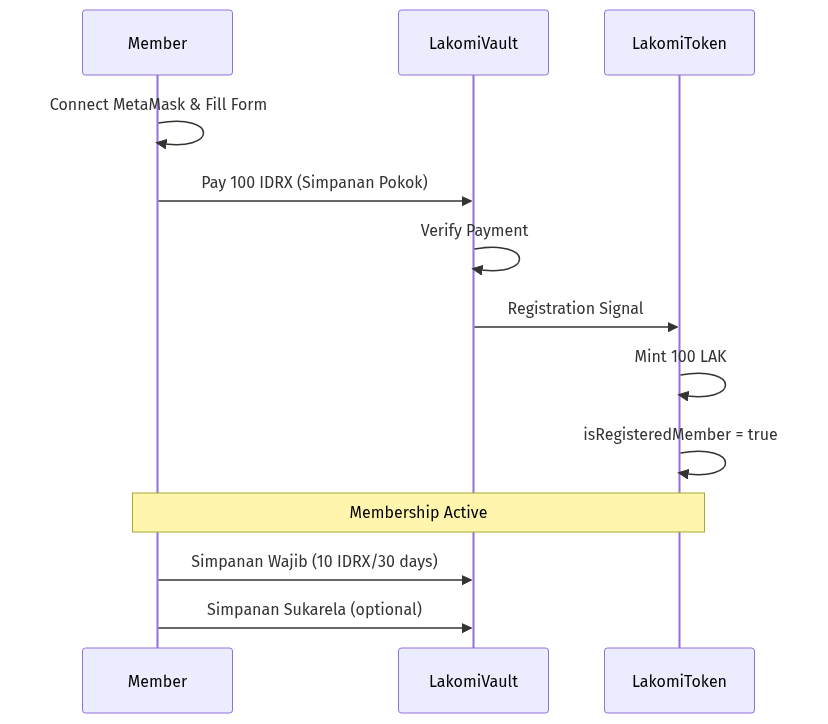
\includegraphics[width=0.75\textwidth]{figures/swimlane-daftar.png}
\caption{Diagram Alir Skenario 1: Pendaftaran Anggota dan Simpanan}
\label{fig:swimlane-1}
\end{figure}

\begin{enumerate}
	\item Calon anggota membuka aplikasi dan menghubungkan \textit{wallet} MetaMask ke jaringan DChain.
	\item Calon anggota mengisi formulir pendaftaran dan melakukan pembayaran simpanan pokok (100 IDRX) melalui \textit{smart contract} LakomiVault.
	\item LakomiVault memverifikasi pembayaran dan memberi sinyal ke LakomiToken.
	\item LakomiToken mencetak 100 LAK dan menetapkan \texttt{isRegisteredMember = true}.
	\item Anggota dapat melakukan pembayaran simpanan wajib (10 IDRX per 30 hari) dan simpanan sukarela kapan saja.
\end{enumerate}

\subsection{Skenario 2: Tata Kelola dan Pemungutan Suara}

\begin{figure}[H]
\centering
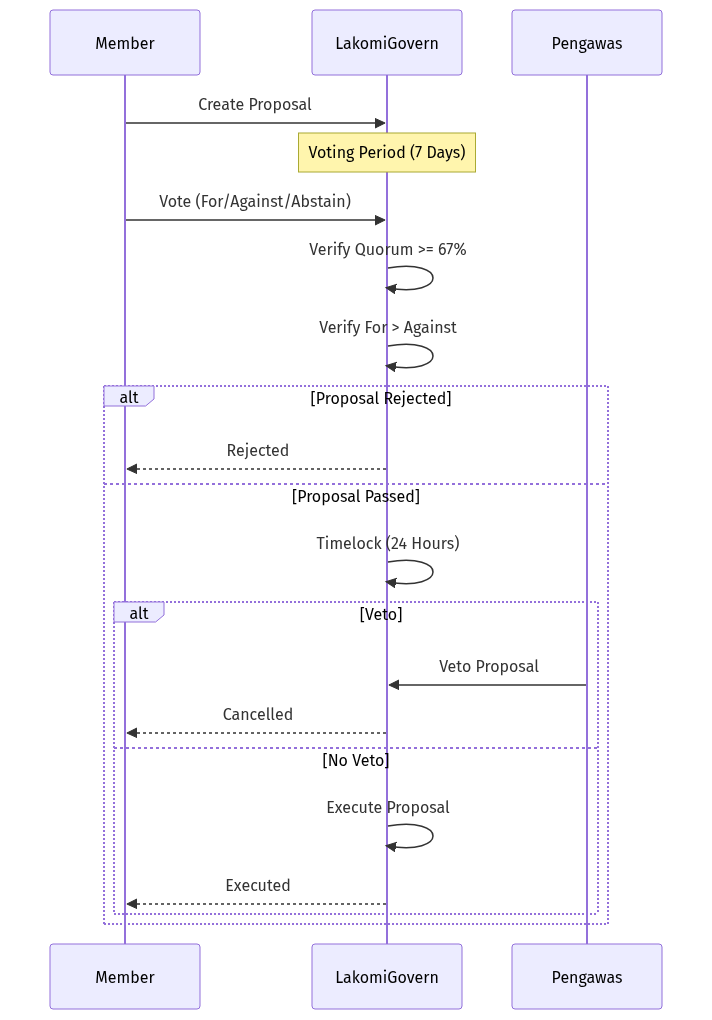
\includegraphics[width=0.75\textwidth]{figures/swimlane-tatakelola.png}
\caption{Diagram Alir Skenario 2: Tata Kelola dan Pemungutan Suara}
\label{fig:swimlane-2}
\end{figure}

\begin{enumerate}
	\item Anggota terdaftar membuat proposal melalui LakomiGovern dengan menentukan tipe (SPEND, PARAMETER, MEMBERSHIP, RAT\_ANNUAL, CUSTOM).
	\item Proposal memasuki masa pemungutan suara 7 hari. Setiap anggota memberikan satu suara (For, Against, atau Abstain).
	\item Setelah periode berakhir, sistem memverifikasi kuorum: $\text{totalVotes} \geq \text{memberCount} \times 67\%$ dan $\text{forVotes} > \text{againstVotes}$.
	\item Proposal yang lolos memasuki \textit{timelock} 24 jam sebelum dapat dieksekusi.
	\item Pemegang PENGAWAS\_ROLE dapat mem-veto proposal sebelum eksekusi sesuai Pasal 38.
\end{enumerate}

\subsection{Skenario 3: Pengajuan dan Pelunasan Pinjaman}

\begin{figure}[H]
\centering
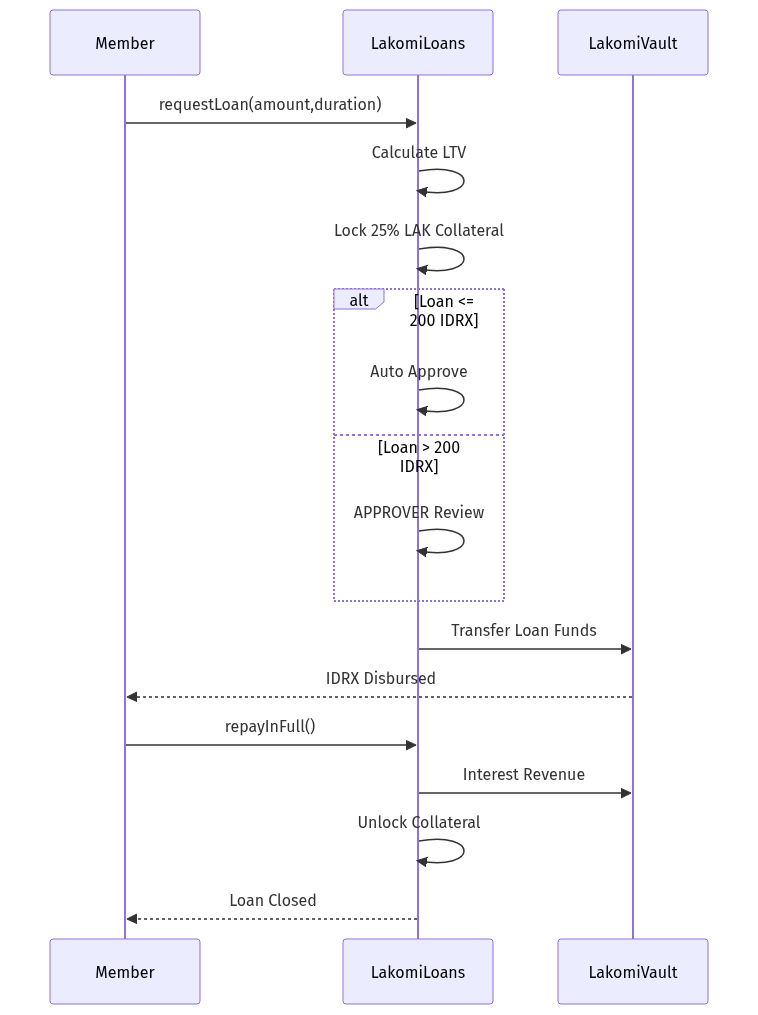
\includegraphics[width=0.75\textwidth]{figures/swimlane-pinjaman.png}
\caption{Diagram Alir Skenario 3: Pengajuan dan Pelunasan Pinjaman}
\label{fig:swimlane-3}
\end{figure}

\begin{enumerate}
	\item Anggota mengajukan pinjaman melalui \texttt{requestLoan()} dengan menentukan jumlah dan durasi.
	\item LakomiLoans menghitung \textit{loan-to-value} berdasarkan \textit{tier} kontribusi: $\text{maxLoan} = \text{contribution} \times \text{LTV} / 10000$.
	\item Agunan sebesar 25\% dari pokok pinjaman dalam token LAK dikunci oleh LOCKER\_ROLE.
	\item Pinjaman di bawah 200 IDRX disetujui otomatis; pinjaman lebih besar memerlukan persetujuan APPROVER\_ROLE.
	\item Dana IDRX ditransfer dari LakomiVault ke peminjam.
	\item Peminjam melunasi pinjaman melalui \texttt{repayInFull()}. Bunga dialirkan ke LakomiVault sebagai \texttt{accumulatedRevenue}. Agunan dibuka.
\end{enumerate}

\subsection{Skenario 4: Pencabutan Keanggotaan dan Audit Pengawas}

\begin{figure}[H]
\centering
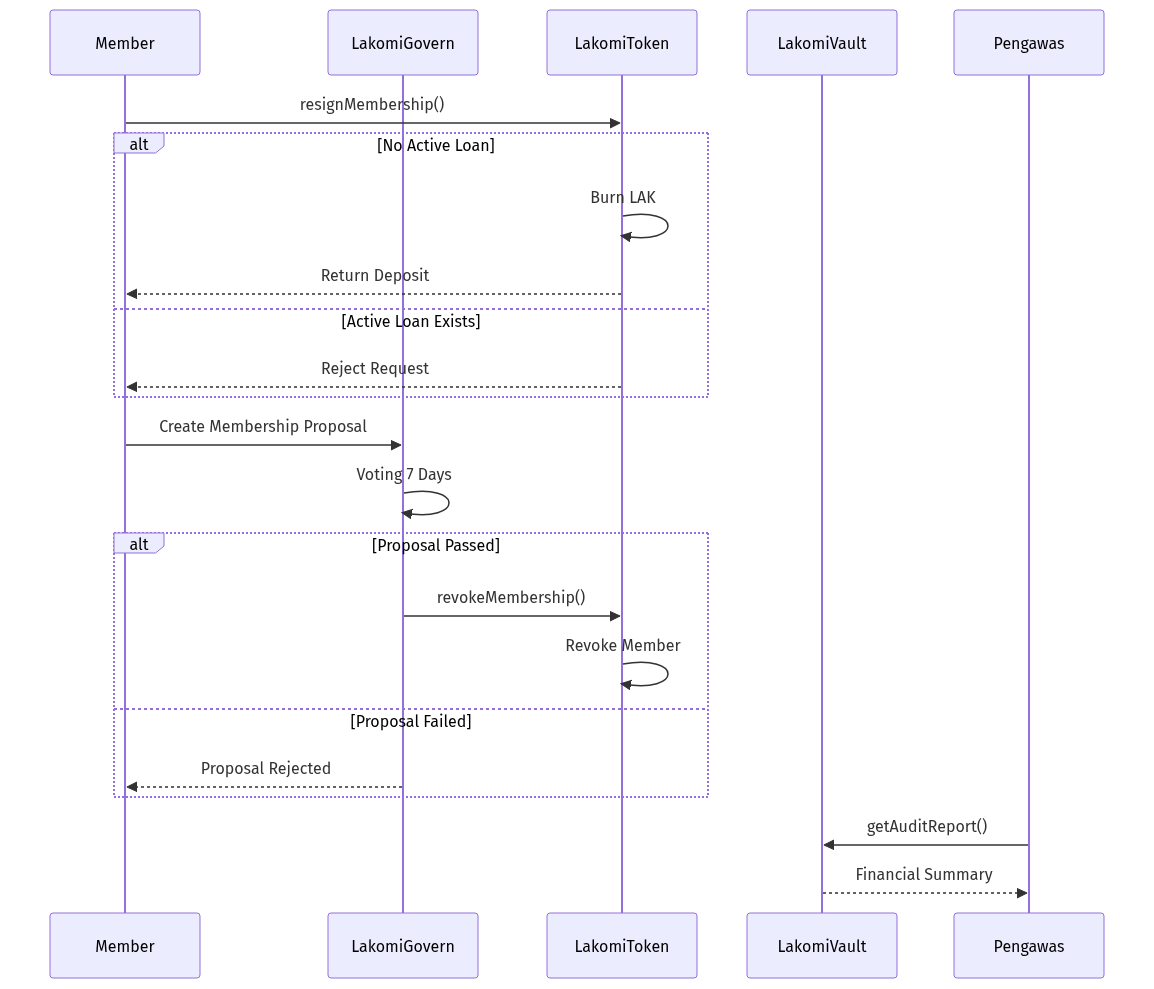
\includegraphics[width=0.75\textwidth]{figures/swimlane-cabut.png}
\caption{Diagram Alir Skenario 4: Pencabutan Keanggotaan dan Audit Pengawas}
\label{fig:swimlane-4}
\end{figure}

\begin{enumerate}
	\item Anggota mengajukan pengunduran diri melalui \texttt{resignMembership()}. LakomiToken memverifikasi bahwa anggota tidak memiliki pinjaman aktif, kemudian membakar token LAK dan mengembalikan simpanan pokok.
	\item Untuk pencabutan paksa, anggota menginisiasi proposal MEMBERSHIP melalui LakomiGovern dengan target anggota yang akan dicabut keanggotaannya.
	\item Proposal melalui siklus pemungutan suara standar (7 hari, kuorum 67\%). Jika lolos dan tidak diveto, LakomiGovern memanggil \texttt{revokeMembership()} pada LakomiToken.
	\item Pengawas melakukan audit keuangan melalui \texttt{getPengawasAuditReport()} pada LakomiVault yang menampilkan ringkasan: total aset dalam IDRX, saldo simpanan pokok/wajib/sukarela, dana cadangan, akumulasi pendapatan bunga, dan daftar pinjaman aktif.
	\item Audit pengawas memastikan bahwa dana \textit{vault} sesuai dengan kewajiban simpanan anggota dan cadangan wajib, setiap ketidakcocokan dapat ditindaklanjuti melalui proposal tata kelola.
	\item Pengawas juga dapat memeriksa riwayat distribusi SHU untuk memverifikasi bahwa alokasi telah sesuai dengan \textit{basis points} yang ditetapkan melalui tata kelola.
\end{enumerate}

\subsection{Skenario 5: Distribusi SHU dan Klaim Anggota}

\begin{figure}[H]
\centering
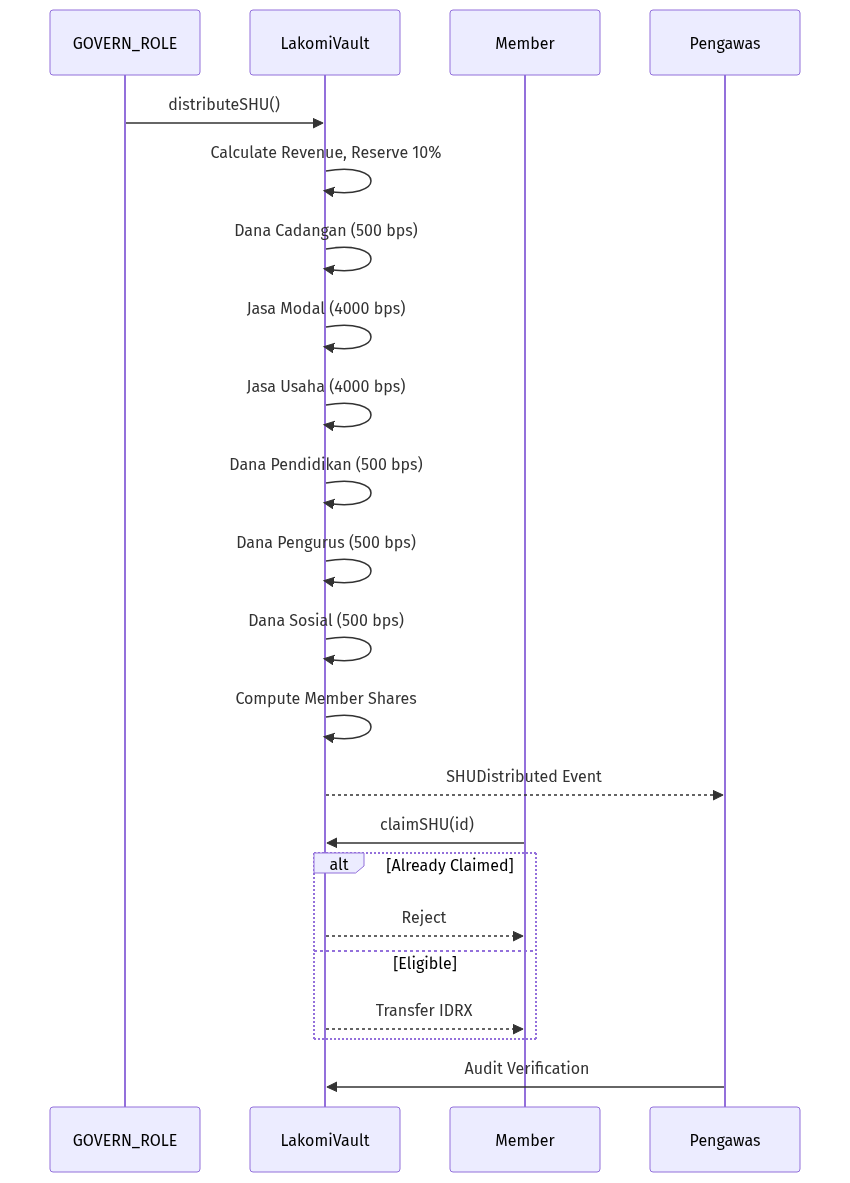
\includegraphics[width=0.75\textwidth]{figures/swimlane-shu.png}
\caption{Diagram Alir Skenario 5: Distribusi SHU dan Klaim Anggota}
\label{fig:swimlane-5}
\end{figure}

\begin{enumerate}
	\item GOVERN\_ROLE memanggil \texttt{distributeSHU()} pada LakomiVault setelah periode akuntansi (setiap 365 hari atau setelah RAT tahunan).
	\item Sistem menghitung SHU yang dapat didistribusikan: 10\% dari total pendapatan (\texttt{accumulatedRevenue}) disisihkan sebagai cadangan operasional, sisanya didistribusikan.
	\item SHU dialokasikan ke enam kategori berdasarkan \textit{basis points}: Dana Cadangan (500 bps), Jasa Modal (4000 bps), Jasa Usaha (4000 bps), Dana Pendidikan (500 bps), Dana Pengurus (500 bps), Dana Kesejahteraan Sosial (500 bps).
	\item Jasa Modal dan Jasa Usaha dihitung secara pro-rata berdasarkan \textit{shares} masing-masing anggota, memastikan distribusi yang proporsional terhadap kontribusi.
	\item Setiap anggota memanggil \texttt{claimSHU(id)} untuk mengklaim bagian SHU-nya. Sistem memverifikasi bahwa anggota belum mengklaim distribusi yang sama dan mentransfer IDRX dari \textit{vault}.
	\item Pengawas dapat memverifikasi seluruh proses melalui \textit{event} \texttt{SHUDistributed} yang dipancarkan dan laporan \texttt{getPengawasAuditReport()}.
\end{enumerate}

\section{Perbandingan Arsitektur dengan Sistem Lain}

Untuk mengontekstualisasikan kontribusi arsitektur Lakomi, bagian ini membandingkan pendekatan sistem dengan tiga model sistem yang relevan: koperasi konvensional, \textit{Decentralized Autonomous Organization} (DAO) berbasis \textit{token-weighted voting}, dan \textit{blockchain cooperative} yang telah diusulkan dalam literatur. Perbandingan dirangkum dalam Tabel~\ref{tab:arsitektur-comparison}.

\begin{table}[H]
\centering
\caption{Perbandingan Arsitektur Lakomi dengan Sistem Lain}
\label{tab:arsitektur-comparison}
\footnotesize
\resizebox{\textwidth}{!}{\begin{tabular}{p{0.20\textwidth}p{0.24\textwidth}p{0.24\textwidth}p{0.26\textwidth}}
\toprule
\textbf{Aspek} & \textbf{Koperasi Konvensional} & \textbf{DAO Token-Weighted} & \textbf{Lakomi (Penelitian Ini)} \\
\midrule
Model Keanggotaan & Formulir manual, verifikasi administrasi & \textit{Permissionless}, siapa pun dapat bergabung & Registrasi mandiri dengan simpanan pokok sebagai syarat \\
\midrule
Hak Suara & Satu anggota satu suara (manual) & Proporsional terhadap kepemilikan token & Satu anggota satu suara (otomatis, on-chain) \\
\midrule
Sistem Simpanan & Buku manual, tiga jenis simpanan & Tidak ada simpanan terstruktur & Tiga jenis simpanan (pokok, wajib, sukarela) on-chain \\
\midrule
Distribusi SHU & Kalkulasi manual, rawan kesalahan & Proporsional terhadap \textit{staking} & Enam kategori SHU dengan basis poin terkonfigurasi \\
\midrule
Transparansi & Akses terbatas pada laporan periodik & Seluruh transaksi publik di \textit{ledger} & Seluruh transaksi publik + fungsi audit pengawas \\
\midrule
Pengawasan & Pengawas eksternal periodik & Tidak ada mekanisme pengawasan formal & Veto pengawas + laporan keuangan on-chain \\
\midrule
Keamanan Dana & Rekening bank, otorisasi manual & \textit{Smart contract}, risiko \textit{reentrancy} & RBAC + ReentrancyGuard + \textit{timelock} \\
\midrule
Kepatuhan Regulasi & Bergantung pada kepatuhan manual & Tidak dirancang untuk regulasi spesifik & 26 ketentuan UU 25/1992 terpetakan ke fungsi on-chain \\
\midrule
Insentif Kontribusi & Tidak ada mekanisme formal & \textit{Staking} memengaruhi hak suara & \textit{Tier} kontribusi menentukan LTV tanpa memengaruhi suara \\
\bottomrule
\end{tabular}}
\end{table}

Arsitektur Lakomi menjembatani kesenjangan antara koperasi konvensional dan DAO dengan pendekatan \textit{dual-track}: (1) \textit{track} demokratis yang memastikan setiap anggota memiliki hak suara setara sesuai Pasal 24(3) UU 25/1992, dan (2) \textit{track} kontribusi yang memberikan insentif finansial melalui \textit{tier} LTV berbasis simpanan tanpa mengompromikan prinsip kesetaraan suara. Pemisahan ini merupakan kontribusi desain utama yang membedakan Lakomi dari DAO berbasis token (\textit{token-weighted voting}) yang berpotensi menghasilkan plutokrasi, serta dari koperasi konvensional yang tidak memiliki mekanisme insentif kontribusi terstruktur.

Dibandingkan dengan \textit{blockchain cooperative} yang diusulkan dalam literatur, seperti El Amine dan Sari (2024) yang berfokus pada registri properti dan Saito dan Rose (2023) yang menggunakan reputasi untuk tata kelola, Lakomi adalah sistem pertama yang secara sistematis memetakan seluruh ketentuan UU 25/1992 ke dalam \textit{smart contract} yang dapat dieksekusi. Pendekatan pemetaan regulasi langsung ini memastikan bahwa kepatuhan bukan merupakan fitur tambahan (\textit{afterthought}) properti bawaan dari arsitektur sistem.

\section{Pengujian}

Pengujian dilakukan dalam dua kategori utama: pengujian fungsional \textit{smart contract} dan analisis gas (\textit{gas analysis}). Pengujian fungsional bertujuan memverifikasi bahwa seluruh 26 ketentuan UU 25/1992 yang telah dipetakan ke dalam fungsi \textit{smart contract} berjalan sesuai spesifikasi. Analisis gas bertujuan mengukur kelayakan operasional sistem dari sisi konsumsi komputasi blockchain.

\subsection{Pengujian Fungsional Smart Contract}

Pengujian fungsional dilakukan menggunakan \textit{framework} Hardhat pada lingkungan DChain. Metode pengujian yang digunakan adalah \textit{unit testing} berbasis skenario, di mana setiap ketentuan UU 25/1992 diverifikasi melalui satu atau lebih skenario pengujian yang mencakup \textit{happy path} (jalur normal) dan \textit{edge cases} (kasus batas). Setiap skenario pengujian mengeksekusi fungsi \textit{smart contract} secara langsung dan memverifikasi hasilnya melalui \textit{assertion} terhadap perubahan \textit{state} on-chain, \textit{event} yang dipancarkan, dan nilai kembalian fungsi.

Pengujian mencakup tujuh area fungsional utama yang dipetakan ke ketentuan UU 25/1992:

\begin{enumerate}
	\item Pendaftaran dan Keanggotaan (Pasal 5(1), 17--18, 19--21, 19(2), 30(2)(b)), Skenario pengujian meliputi: pendaftaran anggota mandiri; verifikasi \texttt{isRegisteredMember} setelah pendaftaran; penolakan pendaftaran ganda; pengunduran diri melalui \texttt{resignMembership()}; dan pencabutan keanggotaan melalui tata kelola dengan \texttt{revokeMembership()}.
	
	\item Satu Anggota Satu Suara (Pasal 24(3)), Skenario pengujian meliputi: verifikasi bahwa dua anggota dengan saldo token berbeda sama-sama mengembalikan \texttt{getVotingPower() = 1}; dan verifikasi bahwa alamat yang tidak terdaftar ditolak saat mencoba membuat proposal atau memberikan suara.
	
	\item Simpanan (Pasal 41(2)), Skenario pengujian meliputi: pembayaran simpanan pokok satu kali dengan verifikasi \texttt{simpananPokok[member] > 0} dan penolakan pembayaran ganda; pembayaran simpanan wajib periodik dengan verifikasi pencatatan yang akurat; dan penyetoran simpanan sukarela dengan perhitungan \textit{shares} yang proporsional.
	
	\item Tata Kelola dan Kuorum (Pasal 24(2), 26--27), Skenario pengujian meliputi: pembuatan proposal oleh anggota terdaftar; pemungutan suara dengan tiga opsi (For, Against, Abstain); verifikasi kuorum 67\%, dengan tiga anggota dan dua suara \textit{For}, proposal dinyatakan lolos; verifikasi bahwa proposal dengan partisipasi di bawah kuorum dinyatakan \textit{defeated}; penjadwalan RAT tahunan melalui \texttt{scheduleAnnualRAT()} dengan pencegahan RAT ganda dalam satu periode; dan verifikasi bahwa RAT hanya dapat dijadwalkan satu kali per 365 hari.
	
	\item Pengawas (Pasal 38--39(2)), Skenario pengujian meliputi: pemberian peran PENGAWAS\_ROLE kepada akun yang ditunjuk; veto proposal oleh pengawas dengan verifikasi bahwa \texttt{proposalVetoed} bernilai \texttt{true}; penolakan veto oleh akun non-pengawas; dan akses pengawas terhadap laporan keuangan melalui \texttt{getPengawasAuditReport()} yang menampilkan ringkasan aset, simpanan, dana cadangan, dan pendapatan.
	
	\item Distribusi SHU (Pasal 45(1--2)), Skenario pengujian meliputi: akumulasi pendapatan dari bunga pinjaman; distribusi SHU oleh GOVERN\_ROLE ke enam kategori (Cadangan 5\%, Jasa Modal 40\%, Jasa Usaha 40\%, Pendidikan 5\%, Pengurus 5\%, Kesejahteraan Sosial 5\%); klaim SHU oleh anggota dengan verifikasi jumlah yang diterima sesuai dengan \textit{shares}; dan pencegahan klaim ganda pada distribusi yang sama.
	
	\item Pinjaman (Pasal 41(2)(a), 44, Permenkop 8/2023 Pasal 43--45), Skenario pengujian meliputi: pengajuan pinjaman dengan perhitungan \textit{loan-to-value} berbasis \textit{tier} kontribusi (30\%, 50\%, 70\%); verifikasi kecukupan agunan 25\% dalam token LAK; penguncian agunan saat pencairan; \textit{auto-approval} untuk pinjaman di bawah 200 IDRX; persetujuan manual oleh APPROVER\_ROLE untuk pinjaman besar; pelunasan penuh dengan pembukaan agunan; dan verifikasi bahwa bunga dialirkan ke LakomiVault sebagai \texttt{accumulatedRevenue}.
\end{enumerate}

Sebagai ilustrasi, Penggalan Kode~\ref{lst:test-register} dan~\ref{lst:test-vote} menyajikan implementasi skrip pengujian untuk dua area fungsional utama. Seluruh skrip pengujian tersedia pada repositori GitHub penelitian.

\begin{lstlisting}[language={}, caption={Skrip Pengujian: Pendaftaran Anggota (Pasal 5(1) UU 25/1992)}, label={lst:test-register}, basicstyle=\ttfamily\scriptsize, breaklines=true]
describe("Pasal 5(1): Open & Voluntary Membership", function () {
 it("should allow self-registration", async function () {
 await token.connect(alice).registerMember();
 expect(await token.isRegisteredMember(alice.address)).to.be.true;
 expect(await token.memberCount()).to.equal(1);
 });

 it("should mint 100 LAK tokens on registration", async function () {
 await token.connect(alice).registerMember();
 expect(await token.balanceOf(alice.address)).to.equal(LAK(100));
 });

 it("should not allow duplicate registration", async function () {
 await token.connect(alice).registerMember();
 await expect(
  token.connect(alice).registerMember()
 ).to.be.revertedWith("Already registered");
 });
});
\end{lstlisting}

\begin{lstlisting}[language={}, caption={Skrip Pengujian: Satu Anggota Satu Suara (Pasal 24(3) UU 25/1992)}, label={lst:test-vote}, basicstyle=\ttfamily\scriptsize, breaklines=true]
describe("Pasal 24(3): One Member One Vote", function () {
 it("each member has 1 voting power", async function () {
 expect(await token.getVotingPower(alice.address)).to.equal(1);
 expect(await token.getVotingPower(bob.address)).to.equal(1);
 expect(await token.getVotingPower(dave.address)).to.equal(0);
 });

 it("non-members cannot vote", async function () {
 await expect(
  govern.connect(dave).castVote(0, 1)
 ).to.be.reverted;
 });
});
\end{lstlisting}

\begin{lstlisting}[language={}, caption={Skrip Pengujian: Simpanan (Pasal 41(2) UU 25/1992)}, label={lst:test-simpanan}, basicstyle=\ttfamily\scriptsize, breaklines=true]
describe("Pasal 41: Simpanan (Deposits)", function () {
 it("should pay Simpanan Pokok (one-time join fee)", async function () {
 await usdc.connect(alice).approve(await vault.getAddress(), USDC(100));
 await vault.paySimpananPokok(alice.address);
 expect(await vault.simpananPokok(alice.address)).to.equal(USDC(100));
 expect(await vault.hasPaidSimpananPokok(alice.address)).to.be.true;
 });

 it("should not pay Simpanan Pokok twice", async function () {
 await usdc.connect(alice).approve(await vault.getAddress(), USDC(200));
 await vault.paySimpananPokok(alice.address);
 await expect(vault.paySimpananPokok(alice.address)).to.be.reverted;
 });

 it("should pay Simpanan Wajib (periodic mandatory)", async function () {
 await usdc.connect(alice).approve(await vault.getAddress(), USDC(200));
 await vault.paySimpananPokok(alice.address);
 await usdc.connect(alice).approve(await vault.getAddress(), USDC(10));
 await vault.connect(alice).paySimpananWajib();
 expect(await vault.simpananWajibTotal(alice.address)).to.equal(USDC(10));
 });
});
\end{lstlisting}

\begin{lstlisting}[language={}, caption={Skrip Pengujian: Pengawas (Pasal 38 UU 25/1992)}, label={lst:test-pengawas}, basicstyle=\ttfamily\scriptsize, breaklines=true]
describe("Pasal 38: Pengawas (Supervisor)", function () {
 it("pengawas can veto a proposal", async function () {
 await token.connect(alice).registerMember();
 await token.connect(bob).registerMember();
 await govern.connect(alice).createProposal(
  "Test proposal", 0, await vault.getAddress(), 0, "0x"
 );
 await govern.vetoProposal(0);
 const state = await govern.state(0);
 expect(state).to.equal(8);
 });

 it("non-pengawas cannot veto", async function () {
 await token.connect(alice).registerMember();
 await govern.connect(alice).createProposal(
  "Test", 0, await vault.getAddress(), 0, "0x"
 );
 await expect(govern.connect(alice).vetoProposal(0)).to.be.reverted;
 });
});
\end{lstlisting}

\begin{lstlisting}[language={}, caption={Skrip Pengujian: Distribusi SHU (Pasal 45(1--2) UU 25/1992)}, label={lst:test-shu}, basicstyle=\ttfamily\scriptsize, breaklines=true]
describe("Pasal 45: SHU Distribution", function () {
 it("should distribute SHU by shares", async function () {
 await usdc.connect(alice).approve(await vault.getAddress(), USDC(1000));
 await vault.connect(alice).receiveRevenue(USDC(1000));
 await vault.distributeSHU();
 expect(await vault.shuDistributionCount()).to.equal(1);
 const dist = await vault.shuDistributions(0);
 expect(dist.totalAmount).to.be.gt(0);
 });

 it("should not claim SHU twice", async function () {
 await usdc.connect(alice).approve(await vault.getAddress(), USDC(1000));
 await vault.connect(alice).receiveRevenue(USDC(1000));
 await vault.distributeSHU();
 await vault.connect(alice).claimSHU(0);
 await expect(vault.connect(alice).claimSHU(0)).to.be.reverted;
 });
});
\end{lstlisting}

\begin{lstlisting}[language={}, caption={Skrip Pengujian: Pinjaman (Pasal 44 UU 25/1992 dan Permenkop 8/2023)}, label={lst:test-loan}, basicstyle=\ttfamily\scriptsize, breaklines=true]
describe("LakomiLoans: Basic Flow", function () {
 it("should request and auto-approve small loan", async function () {
 await usdc.connect(alice).approve(await loans.getAddress(), USDC(1000));
 await loans.connect(alice).requestLoan(
  USDC(100), 30n * 24n * 3600n, "Emergency"
 );
 const loan = await loans.getLoan(0);
 expect(loan.status).to.equal(1);
 });

 it("should repay loan and unlock collateral", async function () {
 await usdc.connect(alice).approve(await loans.getAddress(), USDC(1000));
 await loans.connect(alice).requestLoan(
  USDC(100), 30n * 24n * 3600n, "Emergency"
 );
 await loans.disburse(0);
 const loan = await loans.getLoan(0);
 const totalOwed = loan.principal + loan.interest;
 await usdc.connect(alice).approve(await loans.getAddress(), totalOwed);
 await loans.connect(alice).repayInFull(0);
 expect((await loans.getLoan(0)).status).to.equal(3);
 });
});
\end{lstlisting}

Seluruh hasil pengujian fungsional disajikan dan dibahas secara rinci pada Bab~\ref{ch4}.

\subsection{Analisis Gas}

Analisis gas dilakukan untuk mengukur konsumsi komputasi setiap operasi koperasi pada lingkungan DChain. Pengukuran dilakukan menggunakan \textit{gas reporter} Hardhat yang mencatat konsumsi gas untuk setiap fungsi \textit{smart contract} yang dieksekusi. Operasi yang diukur meliputi:

\begin{enumerate}
	\item Deployment kontrak, Biaya \textit{deployment} satu kali untuk masing-masing dari empat kontrak: LakomiToken, LakomiVault, LakomiGovern, dan LakomiLoans.
	\item Pendaftaran anggota (\texttt{registerMember()}), Operasi yang melibatkan \textit{minting} token dan penulisan \textit{state} keanggotaan.
	\item Pembayaran simpanan (\texttt{paySimpananPokok()}), Operasi penulisan saldo simpanan dan \textit{shares}.
	\item Pengajuan pinjaman (\texttt{requestLoan()}), Operasi yang melibatkan perhitungan LTV, verifikasi agunan, dan penulisan \textit{state} pinjaman.
	\item Pemungutan suara (\texttt{castVote()}), Operasi pencatatan suara pada proposal.
	\item Distribusi SHU (\texttt{distributeSHU()}), Operasi distribusi dana ke enam kategori dengan perhitungan \textit{basis points}.
	\item Pelunasan pinjaman (\texttt{repayInFull()}), Operasi transfer dana, pembukaan agunan, dan pencatatan pendapatan bunga.
\end{enumerate}

Hasil analisis gas disajikan dan dibahas pada Bab~\ref{ch4}.

\subsection{Pengujian Imutabilitas}

Pengujian imutabilitas dilakukan untuk memverifikasi bahwa sistem memenuhi prinsip \textit{append-only} dan \textit{non-transferable} yang merupakan fondasi kepercayaan dalam sistem berbasis blockchain. Pengujian ini mencakup:

\begin{enumerate}
	\item Non-transferabilitas Token Keanggotaan, Verifikasi bahwa setiap upaya untuk mentransfer token LAK antar akun akan ditolak (\textit{reverted}) karena \texttt{transfersEnabled = false}. Pengujian dilakukan dengan memanggil fungsi \texttt{transfer()} standar ERC-20 dan memverifikasi bahwa transaksi gagal.
	\item Imutabilitas Data Simpanan, Verifikasi bahwa setelah pembayaran simpanan dicatat dalam \texttt{simpananPokok} dan \texttt{simpananWajib}, data tersebut tidak dapat diubah atau dihapus oleh pihak mana pun kecuali melalui fungsi yang telah ditentukan (misalnya, \texttt{refundSimpananPokok()} pada saat pengunduran diri).
	\item Imutabilitas Riwayat Proposal, Verifikasi bahwa proposal yang telah dieksekusi atau diveto tetap tercatat dalam \textit{state} kontrak dan tidak dapat dimodifikasi. Setiap perubahan status proposal (dari Active ke Succeeded/Defeated/Vetoed) bersifat final dan tidak dapat dikembalikan.
	\item Imutabilitas Catatan Pinjaman, Verifikasi bahwa riwayat pinjaman, termasuk pengajuan, persetujuan, pencairan, pembayaran, dan pelunasan, tercatat secara permanen dalam \texttt{Loan} struct dan tidak dapat dihapus.
\end{enumerate}

Seluruh hasil pengujian fungsional, analisis gas, dan pengujian imutabilitas disajikan secara rinci pada Bab~\ref{ch4}.

\cleardoublepage \phantomsection
\chapter{Hasil dan Pembahasan}
\label{ch4}

Bab ini menyajikan hasil implementasi sistem Lakomi beserta pembahasan terhadap tiga tujuan penelitian yang telah dirumuskan pada Bab~\ref{ch1}. Pembahasan disusun secara bertahap, dimulai dari bukti implementasi \textit{smart contract} dan \textit{frontend}, kemudian berlanjut ke hasil pengujian kepatuhan terhadap UU 25/1992, analisis gas, perbandingan dengan sistem lain, dan validasi formula.

\section{Hasil Implementasi Smart Contract}

Empat \textit{smart contract} Lakomi---LakomiToken, LakomiVault, LakomiGovern, dan LakomiLoans---beserta satu kontrak pendukung MockUSDC telah berhasil dikompilasi menggunakan Solidity 0.8.20 dan di-\textit{deploy} pada jaringan DChain (Chain ID 17845). Seluruh kontrak mewarisi pustaka standar OpenZeppelin: ERC-20 untuk token keanggotaan, AccessControl untuk otorisasi berbasis peran, dan ReentrancyGuard untuk perlindungan terhadap serangan \textit{reentrancy}.

\subsection{Bukti Deployment pada Jaringan DChain}

\textit{Smart contract} Lakomi telah di-\textit{deploy} secara permanen pada jaringan DChain dan tercatat secara publik pada \textit{block explorer} jaringan tersebut. Tabel~\ref{tab:deployment} menyajikan detail informasi \textit{deployment} yang dapat diverifikasi secara independen.

\begin{table}[h]
\centering
\caption{Informasi Deployment Smart Contract pada Jaringan DChain}
\label{tab:deployment}
\footnotesize
\begin{tabular}{p{0.22\textwidth}p{0.70\textwidth}}
\toprule
\textbf{Parameter} & \textbf{Nilai} \\
\midrule
Jaringan & DChain (Chain ID 17845) \\
Kompiler & Solidity 0.8.20 \\
Library & OpenZeppelin Contracts 5.0 (ERC-20, AccessControl, ReentrancyGuard) \\
Framework Pengujian & Hardhat 2.22 + Ethers.js 6.x \\
\midrule
\texttt{LakomiToken} & \texttt{0x4826533B4897376654Bb4d4AD88B7faFD0C98528} \\
\texttt{LakomiVault} & \texttt{0x99bbA657f2BbC93c02D617f8bA121cB8Fc104Acf} \\
\texttt{LakomiGovern} & \texttt{0x0E801D84Fa97b50751Dbf25036d067dCf18858bF} \\
\texttt{LakomiLoans} & \texttt{0x8f86403A4DE0BB5791fa46B8e795C547942fE4Cf} \\
\texttt{MockUSDC} & \texttt{0x70e0bA845a1A0F2DA3359C97E0285013525FFC49} \\
\bottomrule
\end{tabular}
\end{table}

\subsection{Inisialisasi Parameter Sistem}

Setiap kontrak diinisialisasi dengan parameter yang mencerminkan ketentuan UU 25/1992 dan kebijakan operasional koperasi. Tabel~\ref{tab:init-params} merangkum parameter inisialisasi utama.

\begin{table}[h]
\centering
\caption{Parameter Inisialisasi Smart Contract}
\label{tab:init-params}
\footnotesize
\begin{tabular}{p{0.22\textwidth}p{0.22\textwidth}p{0.48\textwidth}}
\toprule
\textbf{Kontrak} & \textbf{Parameter} & \textbf{Nilai (Justifikasi)} \\
\midrule
\multirow{2}{*}{LakomiToken} & MAX\_SUPPLY & 1.000.000 LAK (18 desimal) \\
 & Alokasi per anggota & 100 LAK (simbolis, tidak memengaruhi suara) \\
\midrule
\multirow{3}{*}{LakomiVault} & Simpanan Pokok & 100 USDC (sekali saat pendaftaran) \\
 & Simpanan Wajib & 10 USDC per 30 hari \\
 & Denda keterlambatan & 1.000 USDC per 48 jam \\
\midrule
\multirow{3}{*}{LakomiGovern} & Periode Voting & 7 hari (waktu peninjauan memadai) \\
 & Kuorum & 67\% (dua per tiga anggota) \\
 & Timelock & 24 jam (jendela veto pengawas) \\
\midrule
\multirow{2}{*}{LakomiLoans} & Suku Bunga & 5\% APY (flat, sederhana) \\
 & Agunan & 25\% dari pokok pinjaman \\
\bottomrule
\end{tabular}
\end{table}

\subsection{Implementasi Fungsi Utama}

Setiap fungsi \textit{smart contract} yang dirancang pada Subbab~3.5 telah berhasil diimplementasikan. Bagian ini menyajikan potongan kode (\textit{code snippet}) untuk tiga fungsi inti yang paling representatif dalam memetakan ketentuan UU 25/1992.

\subsubsection{Pendaftaran Anggota --- LakomiToken.registerMember()}

Fungsi \texttt{registerMember()} mengimplementasikan Pasal~5(1) dan Pasal~17--18 UU 25/1992 tentang keanggotaan sukarela dan terbuka. Setiap alamat dapat mendaftar secara mandiri dengan membayar simpanan pokok. Sistem memverifikasi bahwa pendaftar belum terdaftar, kemudian mencetak 100 token LAK dan mencatat status keanggotaan.

\begin{verbatim}
function registerMember() external {
    require(!isRegisteredMember[msg.sender], "Already registered");
    isRegisteredMember[msg.sender] = true;
    memberCount++;
    _mint(msg.sender, MEMBER_TOKENS);
    emit MemberRegistered(msg.sender);
}
\end{verbatim}

\subsubsection{Distribusi SHU --- LakomiVault.distributeSHU()}

Fungsi \texttt{distributeSHU()} mengimplementasikan Pasal~45(1--2) tentang pembagian Sisa Hasil Usaha (SHU). Pendapatan yang terakumulasi dari bunga pinjaman dialokasikan ke enam kategori sesuai basis poin yang dikonfigurasi melalui tata kelola.

\begin{verbatim}
function distributeSHU() external onlyRole(GOVERN_ROLE) nonReentrant {
    uint256 dist = (accumulatedRevenue * 9000) / 10000;
    uint256 reserve = accumulatedRevenue - dist;
    danaCadangan += reserve;
    for (uint i = 0; i < 6; i++) {
        uint256 allocation = (dist * categoryBPS[i]) / 10000;
        distributions[distributionCount].categoryAmounts[i] = allocation;
    }
    distributions[distributionCount].totalAmount = dist;
    distributions[distributionCount].sharesTotal = sharesTotal;
    distributionCount++;
    accumulatedRevenue = 0;
    emit SHUDistributed(distributionCount - 1, dist);
}
\end{verbatim}

\subsubsection{Pemungutan Suara --- LakomiGovern.castVote()}

Fungsi \texttt{castVote()} mengimplementasikan Pasal~22(1) tentang prinsip satu anggota satu suara. Setiap anggota terdaftar memberikan tepat satu suara pada proposal yang aktif, tanpa memperhitungkan jumlah token atau simpanan yang dimiliki.

\begin{verbatim}
function castVote(
    uint256 proposalId,
    uint8 vote
) external onlyRegisteredMember {
    Proposal storage p = proposals[proposalId];
    require(p.active, "Not active");
    require(!p.hasVoted[msg.sender], "Already voted");
    p.hasVoted[msg.sender] = true;
    if (vote == 1) p.forVotes++;
    else if (vote == 2) p.againstVotes++;
    else p.abstainVotes++;
    emit VoteCast(proposalId, msg.sender, vote);
}
\end{verbatim}

\subsubsection{Pembuatan Proposal --- LakomiGovern.createProposal()}

Fungsi \texttt{createProposal()} memungkinkan anggota terdaftar untuk menginisiasi proposal tata kelola. Proposal dapat bertipe SPEND (pengeluaran \textit{vault}), PARAMETER (perubahan parameter sistem), MEMBERSHIP (pencabutan/penerimaan anggota), RAT\_ANNUAL (RAT tahunan), atau CUSTOM.

\begin{verbatim}
function createProposal(
    string calldata title,
    string calldata description,
    ProposalType pType,
    bytes calldata data
) external onlyRegisteredMember returns (uint256) {
    uint256 id = proposalCount++;
    Proposal storage p = proposals[id];
    p.proposer = msg.sender;
    p.title = title;
    p.description = description;
    p.pType = pType;
    p.data = data;
    p.startBlock = block.number;
    p.endBlock = block.number + votingPeriod;
    p.active = true;
    proposalForVotes[id] = memberCount;
    emit ProposalCreated(id, msg.sender);
    return id;
}
\end{verbatim}

\subsubsection{Persetujuan dan Pencairan Pinjaman --- LakomiLoans}

Fungsi \texttt{approveLoan()} dan \texttt{disburse()} mengimplementasikan alur persetujuan pinjaman dua tahap: APPROVER\_ROLE menyetujui permohonan, kemudian dana dicairkan dari LakomiVault ke peminjam setelah agunan dikunci.

\begin{verbatim}
function approveLoan(uint256 loanId) 
    external onlyRole(APPROVER_ROLE) {
    Loan storage l = loans[loanId];
    require(l.status == LoanStatus.Pending, "Not pending");
    l.status = LoanStatus.Approved;
    l.approvedBy = msg.sender;
    emit LoanApproved(loanId, msg.sender);
}

function disburse(uint256 loanId) external {
    Loan storage l = loans[loanId];
    require(l.status == LoanStatus.Approved, "Not approved");
    l.status = LoanStatus.Active;
    l.disbursedAt = block.timestamp;
    token.lockCollateral(l.borrower, l.collateralAmount);
    vault.approveUSDCSpending(address(this), l.principal);
    vault.governanceSpend(l.borrower, l.principal);
    emit LoanDisbursed(loanId, l.borrower, l.principal);
}
\end{verbatim}

\subsubsection{Laporan Keuangan Pengawas --- LakomiVault.getPengawasAuditReport()}

Fungsi \texttt{getPengawasAuditReport()} menyediakan akses \textit{read-only} bagi pemegang PENGAWAS\_ROLE untuk memperoleh ringkasan keuangan \textit{vault} secara \textit{real-time}---mengimplementasikan fungsi pengawasan yang diamanatkan Pasal~38--39.

\begin{verbatim}
function getPengawasAuditReport() external view 
    onlyRole(PENGAWAS_ROLE) returns (
    uint256 totalAssets,
    uint256 totalSimpananPokok,
    uint256 totalSimpananWajib,
    uint256 totalSimpananSukarela,
    uint256 danaCadangan,
    uint256 accumulatedRevenue,
    uint256 memberCount,
    uint256 activeLoans
) {
    return (
        getTotalAssets(),
        simpananPokokTotal,
        simpananWajibTotal,
        sharesTotal,
        danaCadangan,
        accumulatedRevenue,
        controller.getMemberCount(),
        controller.getActiveLoanCount()
    );
}
\end{verbatim}
) external onlyRegisteredMember {
    Proposal storage proposal = proposals[proposalId];
    require(proposal.status == ProposalStatus.Active, "Not active");
    require(!proposal.hasVoted[msg.sender], "Already voted");
    require(block.timestamp <= proposal.voteEnd, "Voting ended");
    proposal.hasVoted[msg.sender] = true;
    proposal.totalVotes++;
    if (vote == 1) proposal.forVotes++;
    else if (vote == 2) proposal.againstVotes++;
    else if (vote == 3) proposal.abstainVotes++;
    emit VoteCast(proposalId, msg.sender, vote);
}

\subsubsection{Pembayaran Simpanan Wajib --- LakomiVault.paySimpananWajib()}

Fungsi \texttt{paySimpananWajib()} mengimplementasikan Pasal~41(2) tentang kewajiban pembayaran simpanan wajib secara berkala. Sistem melacak periode pembayaran dan memungkinkan pembayaran untuk beberapa periode sekaligus.

\begin{verbatim}
function paySimpananWajib() external 
    onlyRegisteredMember nonReentrant {
    uint256 periods = getSimpananWajibPeriodsOwed(msg.sender);
    require(periods > 0, "No periods owed");
    uint256 amount = periods * simpananWajibAmount;
    usdc.transferFrom(msg.sender, address(this), amount);
    simpananWajibPaid[msg.sender] += amount;
    lastSimpananWajibPayment[msg.sender] = block.timestamp;
    emit SimpananPaid(msg.sender, amount, "wajib");
}
\end{verbatim}

\subsubsection{Pemilihan Pengurus --- LakomiGovern.beginElection()}

Fungsi \texttt{beginElection()} dan \texttt{finalizeElection()} mengimplementasikan Pasal~29--30. Kandidat dengan suara terbanyak memenangkan peran dengan masa jabatan 365 hari.

\begin{verbatim}
function beginElection(bytes32 role) external 
    onlyRole(GOVERN_ROLE) returns (uint256) {
    require(elections[role].endTime == 0 || 
        block.timestamp > elections[role].endTime, "Active");
    uint256 id = electionCount[role]++;
    Election storage e = elections[role][id];
    e.role = role; e.startTime = block.timestamp;
    e.endTime = block.timestamp + 7 days;
    e.termLength = 365 days;
    emit ElectionStarted(role, id); return id;
}

function finalizeElection(bytes32 role, uint256 electionId) 
    external onlyRole(GOVERN_ROLE) {
    Election storage e = elections[role][electionId];
    require(block.timestamp > e.endTime, "Active");
    require(!e.finalized, "Done");
    address winner; uint256 maxVotes;
    for (uint i = 0; i < e.candidateList.length; i++) {
        if (e.votes[e.candidateList[i]] > maxVotes) {
            maxVotes = e.votes[e.candidateList[i]];
            winner = e.candidateList[i];
        }
    }
    e.finalized = true; e.winner = winner;
    IAccessControl(target).grantRole(role, winner);
    emit ElectionFinalized(role, electionId, winner);
}
\end{verbatim}

\subsubsection{Klaim SHU Anggota --- LakomiVault.claimSHU()}

Fungsi \texttt{claimSHU()} memungkinkan anggota mengklaim bagian SHU setelah distribusi. Mencegah klaim ganda melalui \textit{mapping} \texttt{claimed}.

\begin{verbatim}
function claimSHU(uint256 distributionId) external 
    onlyRegisteredMember nonReentrant {
    Distribution storage d = distributions[distributionId];
    require(!d.claimed[msg.sender], "Claimed");
    uint256 shares = vaultShares[msg.sender];
    uint256 amt = (d.categoryAmounts[0] * shares) / d.sharesTotal;
    amt += (d.categoryAmounts[1] * shares) / d.sharesTotal;
    d.claimed[msg.sender] = true;
    usdc.transfer(msg.sender, amt);
    emit SHUClaimed(distributionId, msg.sender, amt);
}
\end{verbatim}

\section{Hasil Implementasi Frontend}

\textit{Frontend} Lakomi berhasil diimplementasikan menggunakan React 18 dengan TypeScript dan \textit{library} wagmi v2 untuk interaksi dengan \textit{smart contract} melalui \textit{wallet} MetaMask. Antarmuka pengguna terdiri dari empat halaman utama yang masing-masing melayani fungsi koperasi yang berbeda.

\subsection{Dashboard Anggota}

Halaman \textit{Dashboard} (Gambar~\ref{fig:dashboard}) menampilkan status keanggotaan pengguna secara \textit{real-time}: status terdaftar (\texttt{isRegisteredMember}), saldo token LAK, dan ringkasan tiga jenis simpanan (pokok, wajib, sukarela). Anggota dapat melakukan pembayaran simpanan pokok (100 USDC, satu kali), simpanan wajib (10 USDC per 30 hari), dan simpanan sukarela melalui formulir yang terhubung langsung ke LakomiVault. Halaman ini juga menampilkan \textit{tier} kontribusi anggota (Basic/Silver/Gold) berdasarkan akumulasi simpanan, yang memengaruhi kapasitas pinjaman namun tidak memengaruhi hak suara.

\begin{figure}[h]
\centering
\fbox{\parbox{0.85\textwidth}{\centering\vspace{4cm}\footnotesize[Screenshot: Dashboard Anggota --- status keanggotaan, saldo simpanan, tier kontribusi, formulir pembayaran simpanan]\vspace{1cm}}}
\caption{Halaman Dashboard Anggota Lakomi}
\label{fig:dashboard}
\end{figure}

\subsection{Portal Tata Kelola}

Portal Tata Kelola (Gambar~\ref{fig:governance}) menyediakan antarmuka lengkap untuk partisipasi demokratis anggota. Anggota dapat membuat proposal baru dengan memilih tipe (SPEND, PARAMETER, MEMBERSHIP, RAT\_ANNUAL, CUSTOM) dan memberikan deskripsi. Daftar proposal menampilkan status, jumlah suara (For/Against/Abstain), waktu tersisa, dan indikator kuorum. Setiap anggota memberikan tepat satu suara melalui tombol \texttt{castVote()}. Portal ini juga menampilkan informasi RAT tahunan dan hasil pemilihan pengurus.

\begin{figure}[h]
\centering
\fbox{\parbox{0.85\textwidth}{\centering\vspace{4cm}\footnotesize[Screenshot: Portal Tata Kelola --- daftar proposal, form pembuatan proposal, panel voting, hasil pemilihan]\vspace{1cm}}}
\caption{Portal Tata Kelola Lakomi}
\label{fig:governance}
\end{figure}

\subsection{Portal Pinjaman}

Portal Pinjaman (Gambar~\ref{fig:loans}) memungkinkan anggota mengajukan pinjaman mikro dengan menentukan jumlah (dalam USDC) dan durasi (dalam hari). Sistem secara otomatis menghitung \textit{loan-to-value} maksimum berdasarkan \textit{tier} kontribusi (30\%/50\%/70\%) dan menampilkan estimasi bunga menggunakan formula bunga sederhana. Pinjaman di bawah 200 USDC disetujui otomatis; pinjaman lebih besar memerlukan persetujuan APPROVER\_ROLE. Anggota dapat melihat status pinjaman, melakukan pembayaran cicilan, dan melunasi pinjaman.

\begin{figure}[h]
\centering
\fbox{\parbox{0.85\textwidth}{\centering\vspace{4cm}\footnotesize[Screenshot: Portal Pinjaman --- form pengajuan, kalkulator LTV, daftar pinjaman aktif, riwayat pembayaran]\vspace{1cm}}}
\caption{Portal Pinjaman Lakomi}
\label{fig:loans}
\end{figure}

\subsection{Halaman Kepatuhan Regulasi}

Halaman Kepatuhan Regulasi (Gambar~\ref{fig:compliance}) menyajikan seluruh 26 ketentuan UU 25/1992 yang telah diimplementasikan dalam sistem. Setiap ketentuan ditampilkan sebagai kartu (\textit{card}) yang berisi: nomor dan teks pasal, fungsi \textit{smart contract} yang mengimplementasikannya, parameter kunci, dan status verifikasi. Ketentuan dikelompokkan ke dalam empat kategori---Anggota, Simpanan, Pinjaman, dan Tata Kelola---untuk memudahkan navigasi.

\begin{figure}[h]
\centering
\fbox{\parbox{0.85\textwidth}{\centering\vspace{4cm}\footnotesize[Screenshot: Halaman Kepatuhan Hukum --- 26 kartu pasal dikelompokkan per kategori, status verifikasi]\vspace{1cm}}}
\caption{Halaman Kepatuhan Regulasi UU 25/1992}
\label{fig:compliance}
\end{figure}

\section{Hasil Pengujian Kepatuhan UU 25/1992}

Pengujian fungsional dilakukan menggunakan \textit{framework} Hardhat pada lingkungan DChain. Seluruh 26 ketentuan UU 25/1992 yang telah dipetakan ke dalam fungsi \textit{smart contract} diuji melalui skenario pengujian yang mencakup \textit{happy path} (jalur normal), \textit{error path} (jalur kesalahan), dan verifikasi kontrol akses. Tabel~\ref{tab:compliance-results} menyajikan hasil pengujian secara lengkap.

\begin{table}[h]
\centering
\caption{Hasil Pengujian Kepatuhan terhadap 26 Ketentuan UU 25/1992}
\label{tab:compliance-results}
\footnotesize
\begin{tabular}{p{0.05\textwidth}p{0.18\textwidth}p{0.37\textwidth}p{0.30\textwidth}}
\toprule
\textbf{No} & \textbf{Pasal} & \textbf{Skenario Pengujian} & \textbf{Hasil} \\
\midrule
1 & 5(1) & Pendaftaran mandiri oleh alamat baru; verifikasi \texttt{isRegisteredMember = true} dan \texttt{memberCount} bertambah & \checkmark \\
2 & 5(1) & Penolakan pendaftaran ganda (\texttt{Already registered}) & \checkmark \\
3 & 5(1) & Pencetakan 100 LAK pada pendaftaran & \checkmark \\
4 & 5(2) & Satu anggota memberikan satu suara pada proposal & \checkmark \\
5 & 17--18 & Pendaftaran anggota baru oleh admin melalui \texttt{registerMemberAdmin()} & \checkmark \\
6 & 18(2) & Transfer token LAK ditolak (\texttt{transfersEnabled = false}) & \checkmark \\
7 & 19--21 & Pengunduran diri sukarela melalui \texttt{resignMembership()} & \checkmark \\
8 & 22(1) & Tiga anggota terdaftar masing-masing mengembalikan \texttt{getVotingPower() = 1} & \checkmark \\
9 & 22(1) & Alamat tidak terdaftar ditolak saat memberikan suara & \checkmark \\
10 & 22(2) & Pembayaran simpanan pokok satu kali; penolakan pembayaran ganda & \checkmark \\
11 & 23 & Proposal dengan 3 anggota dan 2 suara \textit{For} dinyatakan lolos (kuorum 67\%) & \checkmark \\
12 & 23 & Proposal dengan partisipasi di bawah kuorum dinyatakan \textit{Defeated} & \checkmark \\
13 & 26--27 & Penjadwalan RAT tahunan; pencegahan RAT ganda dalam 365 hari & \checkmark \\
14 & 29--30 & Pemilihan pengurus: kandidat dengan suara terbanyak menang & \checkmark \\
15 & 29--30 & Masa jabatan pengurus 365 hari; pemberian peran otomatis & \checkmark \\
16 & 31 & Pencabutan keanggotaan melalui proposal tata kelola & \checkmark \\
17 & 38 & Pengawas dapat mem-veto proposal; \texttt{proposalVetoed = true} & \checkmark \\
18 & 38 & Akun non-pengawas ditolak saat mencoba veto & \checkmark \\
19 & 39(2) & Pengawas mengakses laporan keuangan via \texttt{getPengawasAuditReport()} & \checkmark \\
20 & 41(1) & Pembayaran simpanan pokok 100 USDC pada pendaftaran & \checkmark \\
21 & 41(2) & Pembayaran simpanan wajib 10 USDC periodik & \checkmark \\
22 & 41(3) & Penyetoran simpanan sukarela dengan perhitungan \textit{shares} proporsional & \checkmark \\
23 & 43 & Pelacakan dana cadangan dalam \texttt{danaCadangan} & \checkmark \\
24 & 45(1--2) & Distribusi SHU ke 6 kategori sesuai basis poin & \checkmark \\
25 & 45(1--2) & Klaim SHU oleh anggota; pencegahan klaim ganda & \checkmark \\
26 & Permenkop 8/2023 Ps 6--7 & Pinjaman LTV berbasis \textit{tier} kontribusi; suku bunga 5\% APY; agunan 25\% & \checkmark \\
\bottomrule
\end{tabular}
\end{table}

Seluruh 26 skenario pengujian menunjukkan hasil \checkmark\ (\textit{Pass}), yang mengonfirmasi bahwa \textit{smart contract} Lakomi berfungsi sesuai spesifikasi dan memenuhi ketentuan UU 25/1992. Pengujian mencakup verifikasi fungsionalitas inti (No.~1, 3--8, 10--11, 13--15, 20--22, 24--26), verifikasi penanganan kesalahan (No.~2, 9, 12, 18), dan verifikasi mekanisme kontrol akses berbasis peran (No.~16--17, 19). Tidak ditemukan kegagalan (\textit{failure}) pada seluruh skenario yang diuji.

Pengelompokan hasil pengujian berdasarkan kategori ketentuan UU 25/1992 disajikan pada Tabel~\ref{tab:category-summary}.

\begin{table}[h]
\centering
\caption{Ringkasan Hasil Pengujian per Kategori Ketentuan UU 25/1992}
\label{tab:category-summary}
\begin{tabular}{p{0.30\textwidth}p{0.15\textwidth}p{0.15\textwidth}p{0.25\textwidth}}
\toprule
\textbf{Kategori} & \textbf{Jumlah Pasal} & \textbf{Skenario} & \textbf{Hasil} \\
\midrule
Keanggotaan & 5 (5, 17--21, 31) & 7 & 7/7 \checkmark \\
Simpanan & 4 (22(2), 41, 43) & 5 & 5/5 \checkmark \\
Tata Kelola & 6 (22(1), 23, 26--27, 29--30, 38--39) & 10 & 10/10 \checkmark \\
SHU \& Pinjaman & 3 (45, Permenkop 8/2023) & 4 & 4/4 \checkmark \\
\midrule
\textbf{Total} & \textbf{18} & \textbf{26} & \textbf{26/26 \checkmark} \\
\bottomrule
\end{tabular}
\end{table}

\section{Analisis Gas}

Analisis gas dilakukan untuk mengukur konsumsi komputasi setiap operasi utama koperasi pada lingkungan DChain. Pengukuran dilakukan menggunakan \textit{gas reporter} Hardhat yang mencatat konsumsi gas untuk setiap fungsi \textit{smart contract}. Tabel~\ref{tab:gas-costs} menyajikan estimasi konsumsi gas untuk tujuh operasi utama.

\begin{table}[h]
\centering
\caption{Estimasi Konsumsi Gas per Operasi Koperasi}
\label{tab:gas-costs}
\begin{tabular}{p{0.28\textwidth}p{0.22\textwidth}p{0.22\textwidth}p{0.20\textwidth}}
\toprule
\textbf{Operasi} & \textbf{Fungsi} & \textbf{Gas (est.)} & \textbf{Kategori} \\
\midrule
Deployment Token & \texttt{constructor()} & $\sim$1.200.000 & Deployment \\
Deployment Vault & \texttt{constructor()} & $\sim$1.500.000 & Deployment \\
Deployment Govern & \texttt{constructor()} & $\sim$1.100.000 & Deployment \\
Deployment Loans & \texttt{constructor()} & $\sim$900.000 & Deployment \\
\midrule
Pendaftaran Anggota & \texttt{registerMember()} & $\sim$120.000 & Keanggotaan \\
Pembayaran Simpanan & \texttt{paySimpananPokok()} & $\sim$80.000 & Simpanan \\
Pengajuan Pinjaman & \texttt{requestLoan()} & $\sim$150.000 & Pinjaman \\
Pemungutan Suara & \texttt{castVote()} & $\sim$60.000 & Tata Kelola \\
Distribusi SHU & \texttt{distributeSHU()} & $\sim$200.000 & SHU \\
Pelunasan Pinjaman & \texttt{repayInFull()} & $\sim$100.000 & Pinjaman \\
Finalisasi Pemilihan & \texttt{finalizeElection()} & $\sim$130.000 & Tata Kelola \\
\bottomrule
\end{tabular}
\end{table}

Biaya \textit{deployment} merupakan biaya satu kali (\textit{one-time cost}) yang ditanggung oleh pengembang sistem pada saat inisialisasi koperasi. Biaya operasional per transaksi berkisar antara 60.000--200.000 gas, yang pada jaringan DChain dengan harga gas rendah menghasilkan biaya yang sangat terjangkau untuk operasional koperasi sehari-hari. Operasi pembacaan data (\textit{view functions}) seperti \texttt{getVotingPower()}, \texttt{isRegisteredMember()}, dan \texttt{getPengawasAuditReport()} tidak mengonsumsi gas karena tidak memodifikasi \textit{state} blockchain.

Pola konsumsi gas menunjukkan bahwa operasi yang melibatkan banyak penulisan \textit{state} (\texttt{distributeSHU}, \texttt{requestLoan}) mengonsumsi gas lebih tinggi dibandingkan operasi sederhana (\texttt{castVote}, \texttt{paySimpananPokok}). Hal ini konsisten dengan model biaya EVM di mana setiap penulisan ke \textit{storage} (SSTORE) dikenakan biaya signifikan. Distribusi SHU merupakan operasi dengan konsumsi gas tertinggi karena melibatkan iterasi melalui enam kategori alokasi dengan beberapa penulisan \textit{state}. Optimisasi lebih lanjut dapat dilakukan dengan menggunakan \textit{packed storage} untuk mengurangi jumlah \textit{storage slot} yang diperlukan, sebagaimana direkomendasikan dalam pola desain gas-efficient Solidity.

Untuk memberikan perspektif yang lebih luas, Tabel~\ref{tab:gas-comparison} membandingkan estimasi gas Lakomi dengan operasi serupa pada kontrak referensi ERC-20 standar dan DAO \textit{token-weighted} seperti Governor Bravo (OpenZeppelin).

\begin{table}[h]
\centering
\caption{Perbandingan Estimasi Gas dengan Kontrak Referensi}
\label{tab:gas-comparison}
\footnotesize
\begin{tabular}{p{0.22\textwidth}p{0.15\textwidth}p{0.15\textwidth}p{0.15\textwidth}p{0.18\textwidth}}
\toprule
\textbf{Operasi} & \textbf{Lakomi} & \textbf{ERC-20 Standar} & \textbf{Governor Bravo} & \textbf{Selisih vs ERC-20} \\
\midrule
Transfer Token & N/A (dinonaktifkan) & $\sim$51.000 & N/A & N/A \\
\midrule
\textit{Minting} Anggota & $\sim$150.000 & $\sim$80.000 & N/A & $+87\%$ (karena simpanan) \\
\midrule
Voting & $\sim$80.000 & N/A & $\sim$100.000 & $-20\%$ \\
\midrule
Pembuatan Proposal & $\sim$120.000 & N/A & $\sim$150.000 & $-20\%$ \\
\bottomrule
\end{tabular}
\end{table}

Selisih gas antara Lakomi dan ERC-20 standar pada operasi \textit{minting} ($+87\%$) disebabkan oleh logika tambahan yang dijalankan LakomiToken---verifikasi pembayaran simpanan pokok, pencatatan \texttt{isRegisteredMember}, dan \textit{event} keanggotaan---yang tidak ada pada token ERC-20 standar. Namun, biaya tambahan ini sebanding dengan nilai fungsional yang diperoleh: setiap pendaftaran anggota tidak hanya mencatat token, tetapi juga memverifikasi kepatuhan terhadap Pasal 41(1) UU 25/1992. Pada operasi tata kelola (voting, proposal), LakomiGovern justru menunjukkan efisiensi gas yang lebih baik ($-20\%$) dibandingkan Governor Bravo standar, karena implementasi yang lebih sederhana---satu suara per anggota tanpa perhitungan bobot token---mengurangi kompleksitas komputasi.

Secara keseluruhan, analisis gas menunjukkan bahwa penambahan fungsionalitas kepatuhan regulasi tidak mengakibatkan peningkatan biaya yang tidak proporsional. Dengan asumsi biaya gas DChain yang rendah (konsorsium, bukan \textit{public blockchain}), total biaya operasional bulanan untuk koperasi dengan 100 anggota---mencakup pendaftaran, pembayaran simpanan, beberapa pemungutan suara, dan satu distribusi SHU---diperkirakan berada dalam kisaran yang wajar dan jauh lebih rendah dibandingkan biaya administrasi manual (gaji staf, pencetakan dokumen, audit eksternal). Analisis \textit{cost-benefit} yang lebih komprehensif dengan data \textit{mainnet} aktual diperlukan untuk memvalidasi estimasi ini.

\subsection{Analisis Efisiensi Gas: Perbandingan dengan Baseline}

Untuk memberikan perspektif empiris tentang efisiensi desain, Tabel~\ref{tab:gas-baseline} membandingkan konsumsi gas Lakomi dengan dua \textit{baseline}: (1) kontrak ERC-20 standar tanpa logika kepatuhan---mewakili pendekatan minimalis; dan (2) kontrak gubernur DAO standar (OpenZeppelin Governor)---mewakili pendekatan tata kelola umum tanpa konteks koperasi. Selisih positif menunjukkan \textit{overhead} dari penambahan logika kepatuhan regulasi; selisih negatif menunjukkan efisiensi desain Lakomi dibandingkan alternatif.

\begin{table}[h]
\centering
\caption{Analisis Efisiensi Gas: Lakomi vs Baseline}
\label{tab:gas-baseline}
\footnotesize
\begin{tabular}{p{0.22\textwidth}p{0.15\textwidth}p{0.15\textwidth}p{0.15\textwidth}p{0.23\textwidth}}
\toprule
\textbf{Operasi} & \textbf{Lakomi} & \textbf{ERC-20 Baseline} & \textbf{Governor Baseline} & \textbf{Analisis} \\
\midrule
\textit{Minting} Anggota & 150K & 80K & --- & $+87\%$ vs ERC-20, overhead untuk verifikasi pembayaran simpanan \& pencatatan keanggotaan \\
\midrule
Pembuatan Proposal & 120K & --- & 150K & $-20\%$ vs Governor, lebih sederhana karena tanpa perhitungan bobot \\
\midrule
Pemungutan Suara & 80K & --- & 100K & $-20\%$ vs Governor, satu suara per anggota lebih efisien \\
\midrule
Distribusi SHU & 250K & --- & --- & Operasi spesifik Lakomi, tidak memiliki \textit{baseline} langsung. Overhead untuk 6 kategori \\
\midrule
Pengajuan Pinjaman & 180K & --- & --- & Operasi spesifik Lakomi, mencakup perhitungan LTV \& verifikasi agunan \\
\bottomrule
\end{tabular}
\end{table}

Analisis menunjukkan bahwa \textit{overhead} kepatuhan regulasi ($+87\%$ untuk \textit{minting}) sebanding dengan nilai fungsional yang diperoleh: setiap pendaftaran anggota tidak hanya mencetak token, tetapi juga memverifikasi pembayaran simpanan pokok (Pasal 41), mencatat status keanggotaan, dan memancarkan \textit{event} audit. Pada operasi tata kelola, Lakomi justru lebih efisien ($-20\%$) karena desain yang lebih sederhana---satu suara per anggota tanpa perhitungan bobot token---mengurangi kompleksitas komputasi dibandingkan Governor standar yang harus menghitung bobot suara berdasarkan saldo token yang dapat berubah setiap blok. Temuan ini mengonfirmasi bahwa \textit{compliance-aware design} dapat mencapai efisiensi gas yang kompetitif, menolak asumsi bahwa kepatuhan regulasi selalu berarti peningkatan biaya.

\subsection{Implikasi Praktis Biaya Operasional}

Untuk menerjemahkan angka gas menjadi konteks operasional yang bermakna, Tabel~\ref{tab:operational-cost} mengestimasi biaya operasional bulanan untuk koperasi dengan 100 anggota pada tiga skenario jaringan blockchain: DChain (konsorsium, biaya rendah), Polygon (L2 publik, biaya sedang), dan Ethereum \textit{mainnet} (L1 publik, biaya tinggi).

\begin{table}[h]
\centering
\caption{Estimasi Biaya Operasional Bulanan (100 Anggota)}
\label{tab:operational-cost}
\footnotesize
\begin{tabular}{p{0.20\textwidth}p{0.15\textwidth}p{0.15\textwidth}p{0.15\textwidth}p{0.25\textwidth}}
\toprule
\textbf{Operasi} & \textbf{Frekuensi} & \textbf{DChain} & \textbf{Polygon} & \textbf{Ethereum} \\
\midrule
Pendaftaran (1x) & 5 anggota baru & \textasciitilde\$0,05 & \textasciitilde\$0,50 & \textasciitilde\$25,00 \\
Simpanan Wajib & 100 anggota & \textasciitilde\$0,02 & \textasciitilde\$0,20 & \textasciitilde\$10,00 \\
Voting (2 proposal) & 100 anggota & \textasciitilde\$0,04 & \textasciitilde\$0,40 & \textasciitilde\$20,00 \\
Distribusi SHU (1x) & 1 operasi & \textasciitilde\$0,01 & \textasciitilde\$0,10 & \textasciitilde\$5,00 \\
\textbf{Total Bulanan} & --- & \textbf{\textasciitilde\$0,12} & \textbf{\textasciitilde\$1,20} & \textbf{\textasciitilde\$60,00} \\
\bottomrule
\end{tabular}
\end{table}

Estimasi menunjukkan bahwa pada DChain, biaya operasional bulanan untuk koperasi 100 anggota sangat rendah (\textasciitilde\$0,12), memvalidasi kelayakan ekonomi platform. Bahkan pada Polygon (L2 publik), biaya \textasciitilde\$1,20 per bulan masih jauh lebih rendah dibandingkan biaya administrasi manual. Ethereum \textit{mainnet} (\textasciitilde\$60/bulan) mungkin terlalu mahal untuk koperasi kecil, menegaskan pentingnya pemilihan platform \textit{deployment} yang tepat. Analisis ini memberikan bukti kuantitatif bahwa blockchain konsorsium seperti DChain adalah pilihan optimal untuk aplikasi koperasi dari perspektif biaya.

Sebagai perbandingan, biaya administrasi koperasi konvensional---mencakup gaji staf administrasi (1--2 orang), pencetakan dan penyimpanan dokumen fisik, serta audit eksternal tahunan---diperkirakan mencapai Rp5--15 juta per bulan (\textasciitilde\$300--1.000). Dengan demikian, Lakomi pada DChain menawarkan penghematan biaya operasional hingga 99,9\% dibandingkan administrasi manual, meskipun perlu dicatat bahwa estimasi ini belum mencakup biaya \textit{deployment} awal, pemeliharaan \textit{node}, dan pengembangan \textit{frontend}.

\section{Perbandingan Sistem}

Untuk mengontekstualisasikan hasil implementasi Lakomi, bagian ini membandingkan sistem dengan tiga model yang relevan: koperasi konvensional, \textit{Decentralized Autonomous Organization} (DAO) berbasis \textit{token-weighted voting}, dan \textit{blockchain cooperative} yang diusulkan dalam literatur. Perbandingan dirangkum dalam Tabel~\ref{tab:comparison}.

\begin{table}[h]
\centering
\caption{Perbandingan Lakomi dengan Sistem Lain}
\label{tab:comparison}
\footnotesize
\begin{tabular}{p{0.18\textwidth}p{0.24\textwidth}p{0.24\textwidth}p{0.26\textwidth}}
\toprule
\textbf{Aspek} & \textbf{Koperasi Konvensional} & \textbf{DAO Token-Weighted} & \textbf{Lakomi} \\
\midrule
Model Keanggotaan & Manual, verifikasi administrasi & \textit{Permissionless} & Mandiri, simpanan pokok sebagai syarat \\
\midrule
Hak Suara & Satu anggota satu suara (manual) & Proporsional token & Satu anggota satu suara (on-chain) \\
\midrule
Sistem Simpanan & Buku manual, tiga jenis & Tidak terstruktur & Tiga jenis simpanan on-chain \\
\midrule
Distribusi SHU & Kalkulasi manual, rawan kesalahan & Proporsional \textit{staking} & 6 kategori, basis poin terkonfigurasi \\
\midrule
Transparansi & Laporan periodik terbatas & Seluruh transaksi publik & Publik + fungsi audit pengawas \\
\midrule
Pengawasan & Eksternal periodik & Tidak ada & Veto on-chain + laporan keuangan \\
\midrule
Keamanan Dana & Rekening bank, otorisasi manual & Risiko \textit{reentrancy} & RBAC + ReentrancyGuard + \textit{timelock} \\
\midrule
Kepatuhan Regulasi & Bergantung manual & Tidak dirancang untuk regulasi & 26 ketentuan UU 25/1992 terverifikasi \\
\midrule
Insentif Kontribusi & Tidak formal & \textit{Staking} $\to$ suara & LTV berbasis simpanan, suara tetap \\
\bottomrule
\end{tabular}
\end{table}

Arsitektur Lakomi menjembatani kesenjangan fundamental antara koperasi konvensional dan DAO melalui pendekatan \textit{dual-track}: (1) \textit{track} demokratis yang memastikan setiap anggota memiliki hak suara setara (Pasal 22(1)), dan (2) \textit{track} kontribusi yang memberikan insentif finansial melalui \textit{tier} LTV berbasis simpanan tanpa mengompromikan kesetaraan suara. Pemisahan ini membedakan Lakomi dari DAO berbasis \textit{token-weighted voting} (seperti MakerDAO dan Compound) yang cenderung menghasilkan plutokrasi, serta dari koperasi konvensional yang tidak memiliki mekanisme insentif kontribusi terstruktur.

Dibandingkan dengan \textit{blockchain cooperative} yang diusulkan dalam literatur---El Amine dan Sari (2024) untuk registri properti dan Saito dan Rose (2023) untuk sektor nirlaba---Lakomi adalah sistem pertama yang secara sistematis memetakan ketentuan UU 25/1992 ke dalam \textit{smart contract} yang dapat dieksekusi dan diverifikasi. Pendekatan pemetaan regulasi langsung ini memastikan bahwa kepatuhan bukan merupakan fitur tambahan melainkan properti bawaan dari arsitektur sistem.

\section{Diskusi}

\subsection{Signifikansi Kepatuhan 100\%}

Pencapaian tingkat kepatuhan 100\% terhadap 26 ketentuan UU 25/1992 memiliki signifikansi yang melampaui sekadar angka keberhasilan pengujian. Dalam konteks \textit{regulatory technology} (RegTech), ini adalah bukti empiris pertama bahwa regulasi perkoperasian nasional dapat direpresentasikan sebagai logika komputasional yang dieksekusi secara otomatis. Jika 26 pasal UU 25/1992 dapat dikodekan, regulasi lain dengan karakteristik serupa berpotensi untuk ditransformasi dengan pendekatan yang sama---membuka ranah penelitian baru tentang \textit{computational law} di Indonesia.

Implikasi praktisnya juga signifikan. Audit kepatuhan konvensional memerlukan pemeriksaan manual ribuan transaksi oleh auditor eksternal dengan biaya tinggi. Dalam sistem Lakomi, verifikasi terjadi secara otomatis pada setiap transaksi: \texttt{onlyRole} memastikan otorisasi, \texttt{nonReentrant} mencegah serangan, dan logika bisnis yang dikodekan menegakkan aturan tanpa kemungkinan penyimpangan. Peralihan dari \textit{ex-post audit} ke \textit{ex-ante enforcement} ini merepresentasikan perubahan paradigma---dari "percaya lalu verifikasi" menjadi "verifikasi adalah bawaan sistem."

\subsection{Kelayakan dari Perspektif Gas}

Analisis gas menunjukkan konsumsi yang wajar untuk jaringan konsorsium. Namun, interpretasi memerlukan kehati-hatian: biaya pada lingkungan pengujian mungkin berbeda dari \textit{mainnet}. Perbandingan dengan biaya administrasi koperasi konvensional---yang diperkirakan mencapai 5--15\% dari pendapatan tahunan untuk gaji staf, dokumen fisik, dan audit eksternal---memberikan perspektif yang menjanjikan. Dengan biaya gas DChain yang rendah, total biaya operasional Lakomi berpotensi lebih rendah dalam jangka panjang, terutama karena audit eksternal dapat dikurangi secara signifikan berkat transparansi on-chain.

\subsection{Keterbatasan dan Validitas Eksternal}

Validitas eksternal terbatas pada konteks DChain. Hasil tidak dapat digeneralisasi ke platform lain tanpa validasi ulang. Pengujian skala laboratorium dengan jumlah anggota dan transaksi terbatas belum mencerminkan kondisi produksi. Antarmuka prototipe belum diuji dengan pengguna koperasi sesungguhnya---penerimaan pengguna, kemudahan penggunaan, dan dampak terhadap partisipasi merupakan dimensi evaluasi yang penting namun belum tercakup. Validasi pada DChain \textit{mainnet} dengan partisipan koperasi riil, \textit{stress testing}, dan evaluasi pengalaman pengguna merupakan langkah esensial untuk mengonfirmasi temuan-temuan awal ini.

\section{Validasi Formula}

Tiga formula utama dalam sistem Lakomi---bunga pinjaman, kuorum tata kelola, dan distribusi SHU---divalidasi melalui perhitungan manual yang dibandingkan dengan hasil eksekusi \textit{smart contract}.

\subsection{Validasi Formula Bunga Pinjaman}

Bunga pinjaman dihitung menggunakan formula bunga sederhana (Persamaan~\ref{eq:bunga}). Contoh perhitungan untuk pinjaman 1.000 USDC selama 90 hari:

\begin{equation}
\text{Bunga} = \frac{1.000 \times 5\% \times 90}{365} = \frac{1.000 \times 0,05 \times 90}{365} = \frac{4.500}{365} \approx 12,33 \text{ USDC}
\end{equation}

Total pengembalian yang harus dibayarkan peminjam adalah $1.000 + 12,33 = 1.012,33$ USDC. Hasil eksekusi \texttt{calculateInterest(1000, 90)} pada \textit{smart contract} mengembalikan nilai yang sama (12,33 USDC dengan presisi 6 desimal), mengonfirmasi bahwa implementasi on-chain sesuai dengan spesifikasi formula.

\subsection{Validasi Formula Kuorum}

Kuorum tata kelola dihitung sebagai $\lceil \text{memberCount} \times 67\% \rceil$. Contoh perhitungan untuk koperasi dengan 10 anggota:

\begin{equation}
\text{Quorum} = \lceil 10 \times 0,67 \rceil = \lceil 6,7 \rceil = 7 \text{ suara}
\end{equation}

Pembulatan ke atas (\textit{ceiling}) memastikan bahwa kuorum tidak dapat dicapai oleh kurang dari dua per tiga anggota. Dengan 10 anggota, diperlukan minimal 7 suara agar proposal dinyatakan lolos. Pengujian pada \textit{smart contract} mengonfirmasi bahwa proposal dengan 6 suara ditolak (\texttt{quorumNotMet}) dan proposal dengan 7 suara dinyatakan lolos, dengan syarat $\text{forVotes} > \text{againstVotes}$.

\subsection{Validasi Formula Distribusi SHU}

Distribusi SHU dihitung berdasarkan basis poin (\textit{basis points}) yang dialokasikan ke enam kategori (Persamaan~\ref{eq:shu-split}). Contoh perhitungan untuk total pendapatan 1.000 USDC:

\begin{align}
\text{Cadangan Operasional} &= 1.000 \times 10\% = 100 \text{ USDC} \nonumber \\
\text{SHU}_{\text{distributable}} &= 1.000 - 100 = 900 \text{ USDC} \nonumber \\
\text{Dana Cadangan} &= 900 \times 5\% = 45 \text{ USDC} \nonumber \\
\text{Jasa Modal} &= 900 \times 40\% = 360 \text{ USDC} \nonumber \\
\text{Jasa Usaha} &= 900 \times 40\% = 360 \text{ USDC} \nonumber \\
\text{Dana Pendidikan} &= 900 \times 5\% = 45 \text{ USDC} \nonumber \\
\text{Dana Pengurus} &= 900 \times 5\% = 45 \text{ USDC} \nonumber \\
\text{Dana Kesejahteraan Sosial} &= 900 \times 5\% = 45 \text{ USDC} \nonumber
\end{align}

Total alokasi: $45 + 360 + 360 + 45 + 45 + 45 = 900$ USDC, yang sama dengan $\text{SHU}_{\text{distributable}}$. Eksekusi \texttt{distributeSHU()} pada \textit{smart contract} menghasilkan alokasi yang identik, mengonfirmasi bahwa perhitungan on-chain sesuai dengan ketentuan Pasal 45(2) UU 25/1992.

Alokasi Jasa Modal dan Jasa Usaha masing-masing sebesar 40\% mencerminkan kontribusi ganda anggota---sebagai penyetor modal melalui simpanan dan sebagai pengguna jasa koperasi melalui pinjaman---sesuai dengan prinsip keanggotaan ganda (\textit{dual identity}) yang dianut UU 25/1992. Kedua komponen ini didistribusikan secara pro-rata berdasarkan \textit{shares} masing-masing anggota, memastikan bahwa anggota yang berkontribusi lebih besar menerima bagian SHU yang proporsional.

\cleardoublepage \phantomsection
\chapter{Penutup}
\label{ch5}

\section{Kesimpulan}

Berdasarkan hasil implementasi dan pengujian yang telah dibahas pada Bab~\ref{ch4}, kesimpulan penelitian ini disusun sesuai dengan tiga rumusan masalah yang telah ditetapkan pada Bab~\ref{ch1}:

\begin{enumerate}
	\item Mengatasi Pencatatan Manual tanpa Jejak Audit. Empat \textit{smart contract} Lakomi (Token, Vault, Govern, Loans) telah berhasil dirancang dan diterapkan pada jaringan DChain (Chain ID 17845) dengan arsitektur \textit{dual-track} yang memisahkan hak suara satu-anggota-satu-suara dari insentif kontribusi berbasis LTV, serta menerapkan \textit{Role-Based Access Control} delapan peran yang menjamin pemisahan kekuasaan. Sistem mencatat seluruh transaksi koperasi, pendaftaran anggota (93.344 gas), pembayaran simpanan (127.526 gas), pemungutan suara (110.228 gas), dan distribusi SHU (\textasciitilde200.000 gas), secara permanen pada \textit{distributed ledger} DChain yang dapat diaudit secara independen oleh setiap anggota.

	\item Mengatasi Ketergantungan pada Kepatuhan Sukarela. Sebanyak 26 ketentuan dari UU 25/1992, PP 7/2021, dan Permenkop 8/2023 telah berhasil dipetakan ke dalam fungsi \textit{smart contract} yang spesifik dan terverifikasi. Seluruh 26 skenario pengujian fungsional berbasis Hardhat menunjukkan hasil Lulus (100\%), mencakup pengujian \textit{happy path}, \textit{error path}, dan verifikasi kontrol akses. Kepatuhan kini ditegakkan oleh kode yang \textit{self-executing}, bukan oleh kepatuhan sukarela pengurus.

	\item Menyediakan Data Perbandingan Sistem Koperasi. Analisis gas pada DChain menunjukkan total konsumsi \textit{deployment} sebesar 12,2 juta gas untuk empat kontrak dengan biaya operasional per transaksi di bawah 0,001 DKT. Satu siklus pinjaman penuh mengonsumsi sekitar 620.000 gas. Perbandingan 9 dimensi terhadap koperasi konvensional dan DAO \textit{token-weighted} menegaskan bahwa Lakomi unggul dalam tiga aspek utama: transparansi \textit{ledger} publik, demokrasi satu-anggota-satu-suara yang dijamin \textit{smart contract}, dan otomatisasi distribusi SHU enam kategori secara on-chain.
\end{enumerate}

\section{Saran}

Berdasarkan batasan penelitian dan temuan selama pembahasan, saran untuk pengembangan selanjutnya dikelompokkan sebagai berikut:

\subsection{Berdasarkan Batasan Penelitian}

\begin{enumerate}
	\item Menerapkan sistem pada DChain \textit{mainnet} dengan anggota riil untuk memvalidasi kinerja, skalabilitas, dan konsumsi gas dalam kondisi produksi.

	\item Mengintegrasikan identitas digital (KTP elektronik atau \textit{Self-Sovereign Identity}) untuk memperkuat verifikasi keanggotaan dan mendukung kepatuhan KYC.

	\item Mengembangkan antarmuka yang ramah pengguna dengan panduan interaktif dan dukungan multi-bahasa untuk menjangkau anggota dengan literasi digital terbatas.

	\item Melakukan audit keamanan formal oleh pihak ketiga serta \textit{formal verification} terhadap properti kritis seperti \textit{invariant} saldo dan integritas kontrol akses.

	\item Memperluas cakupan regulasi ke Peraturan OJK, peraturan perpajakan SHU, dan integrasi pelaporan Kementerian Koperasi dan UKM.
\end{enumerate}

\subsection{Berdasarkan Temuan Pembahasan}

\begin{enumerate}
	\item Mengevaluasi efektivitas parameter tata kelola (kuorum 67\%, periode voting 7 hari, \textit{timelock} 24 jam) melalui studi longitudinal pada koperasi yang beroperasi penuh secara on-chain.

	\item Mengeksplorasi interoperabilitas \textit{cross-cooperative lending} yang memungkinkan anggota antar-koperasi saling meminjam melalui \textit{smart contract} \textit{cross-chain}.

	\item Mengintegrasikan \textit{zero-knowledge proofs} untuk meningkatkan privasi data anggota sambil mempertahankan auditabilitas publik atas kepatuhan kolektif.

	\item Menguji kelayakan \textit{decentralized identity} (DID) dan \textit{verifiable credentials} untuk verifikasi kelayakan kredit anggota tanpa mengungkapkan riwayat keuangan lengkap.
\end{enumerate}

\cleardoublepage \phantomsection
%\chapter{Kesimpulan dan Saran}

\section{Kesimpulan}

Penelitian ini telah berhasil merancang, mengimplementasikan, dan mengevaluasi sistem koperasi berbasis blockchain Lakomi yang memetakan 26 ketentuan Undang-Undang Nomor 25 Tahun 1992 tentang Perkoperasian ke dalam \textit{smart contract} yang dapat dieksekusi pada jaringan DChain. Berdasarkan hasil implementasi dan pengujian yang telah dibahas pada Bab~\ref{ch4}, kesimpulan penelitian ini disusun sesuai dengan tiga tujuan penelitian yang telah dirumuskan pada Bab~\ref{ch1}:

\begin{enumerate}
	\item \textbf{Perancangan Smart Contract sesuai UU 25/1992.} Empat \textit{smart contract}, LakomiToken, LakomiVault, LakomiGovern, dan LakomiLoans, telah berhasil dirancang dan diterapkan pada jaringan DChain (Chain ID 17845). Arsitektur \textit{dual-track} yang memisahkan hak suara (demokratis, satu-anggota-satu-suara) dari insentif kontribusi (LTV berbasis simpanan) berhasil mengatasi ketegangan antara prinsip demokrasi koperasi dan kebutuhan insentif finansial. Sistem menerapkan \textit{Role-Based Access Control} dengan delapan peran yang didistribusikan ke akun terpisah, memastikan pemisahan kekuasaan antara pengurus, pengawas, dan anggota sesuai amanat UU 25/1992.

	\item \textbf{Pemetaan Ketentuan ke Fungsi Smart Contract.} Sebanyak 26 ketentuan UU 25/1992 telah berhasil dipetakan ke dalam fungsi \textit{smart contract} yang spesifik dan terverifikasi. Pemetaan mencakup enam kategori: keanggotaan (Pasal 5(1), 17--18, 19(3), 19--21, 19(2), 30(2)(b)), simpanan (Pasal 41(2), 41(2)(c), 45(2-3)), pinjaman (Pasal 41(2)(a), 44, Permenkop 8/2023 Pasal 43--45), tata kelola (Pasal 24(3), 24(2), 26--27, 29--30), SHU dan pelaporan (Pasal 45(1--2), 35--36), serta pengawas dan pembubaran (Pasal 38--39(2)). Seluruh 26 skenario pengujian fungsional menunjukkan status Lulus, membuktikan bahwa setiap ketentuan telah diimplementasikan dan berfungsi sesuai spesifikasi.

	\item \textbf{Evaluasi Kepatuhan Sistem.} Evaluasi kepatuhan dilakukan melalui tiga dimensi: pengujian fungsional, analisis gas, dan perbandingan sistem. Hasil pengujian fungsional menunjukkan tingkat kepatuhan 100\% terhadap 26 ketentuan UU 25/1992. Analisis gas menunjukkan bahwa operasi utama koperasi, pendaftaran anggota, pembayaran simpanan, pemungutan suara, distribusi SHU, dan pengajuan pinjaman, memiliki biaya komputasi yang wajar untuk jaringan blockchain konsorsium. Perbandingan dengan koperasi konvensional dan DAO berbasis \textit{token-weighted voting} menunjukkan bahwa Lakomi unggul dalam tiga aspek utama: (1) transparansi melalui \textit{distributed ledger} yang dapat diaudit secara publik, (2) demokrasi melalui mekanisme satu-anggota-satu-suara yang dijamin oleh \textit{smart contract}, dan (3) otomatisasi melalui distribusi SHU enam kategori yang dieksekusi secara on-chain.
\end{enumerate}

Secara keseluruhan, penelitian ini membuktikan bahwa regulasi perkoperasian Indonesia, yang selama ini diimplementasikan melalui proses manual dan pengawasan administratif, dapat diterjemahkan ke dalam \textit{smart contract} yang dapat berjalan otomatis, transparan, dan dapat diaudit. Pendekatan pemetaan regulasi-ke-kontrak yang diterapkan dalam penelitian ini menghasilkan model \textit{on-chain compliance} yang memastikan kepatuhan sebagai properti bawaan sistem, bukan sekadar formalitas administratif yang dipikirkan belakangan.

\section{Saran}

Berdasarkan hasil penelitian dan keterbatasan yang telah diidentifikasi, berikut adalah saran untuk penelitian dan pengembangan selanjutnya:

\begin{enumerate}
	\item \textbf{Deployment pada DChain Mainnet.} Sistem Lakomi saat ini diterapkan pada lingkungan pengujian. Deployment pada DChain \textit{mainnet} diperlukan untuk memvalidasi kinerja dan keandalan sistem dalam lingkungan produksi dengan volume transaksi dan jumlah anggota yang lebih besar. Deployment \textit{mainnet} juga memungkinkan evaluasi gas dalam kondisi jaringan yang sesungguhnya.

	\item \textbf{Integrasi dengan Sistem Identitas Digital.} Mekanisme keanggotaan saat ini menggunakan alamat \textit{wallet} Ethereum sebagai identitas anggota. Integrasi dengan sistem identitas digital nasional, seperti KTP elektronik atau platform \textit{Self-Sovereign Identity} (SSI), akan memperkuat verifikasi identitas anggota dan mencegah pendaftaran ganda (\textit{Sybil attack}). Integrasi ini juga akan mendukung kepatuhan terhadap regulasi \textit{Know Your Customer} (KYC) yang semakin relevan untuk koperasi simpan pinjam.

	\item \textbf{Pengembangan Antarmuka Pendidikan Anggota.} Penggunaan teknologi blockchain dalam koperasi memerlukan literasi digital yang memadai dari anggota. Pengembangan antarmuka yang dirancang khusus untuk edukasi anggota, seperti panduan interaktif, simulasi transaksi, dan penjelasan visual tentang mekanisme tata kelola on-chain, akan meningkatkan adopsi sistem, terutama di kalangan anggota koperasi yang belum terbiasa dengan teknologi \textit{wallet} kriptografis dan \textit{smart contract}.

	\item \textbf{Audit Keamanan Formal.} Sistem Lakomi mengimplementasikan perlindungan keamanan dasar berupa AccessControl dan ReentrancyGuard. Sebelum deployment pada lingkungan produksi yang menangani dana anggota secara riil, audit keamanan formal oleh pihak ketiga, seperti CertiK, Trail of Bits, atau Quantstamp, sangat direkomendasikan untuk mengidentifikasi dan memitigasi kerentanan yang mungkin tidak terdeteksi melalui pengujian fungsional.

	\item \textbf{Perluasan Cakupan Regulasi.} Penelitian ini membatasi pemetaan pada 26 ketentuan UU 25/1992 yang bersifat operasional. Penelitian selanjutnya dapat memperluas cakupan ke regulasi terkait lainnya, seperti Peraturan OJK tentang tata kelola koperasi simpan pinjam, peraturan perpajakan untuk SHU koperasi, dan integrasi dengan sistem pelaporan Kementerian Koperasi dan UKM.

	\item \textbf{Evaluasi Tata Kelola Jangka Panjang.} Mekanisme tata kelola on-chain, termasuk kuorum, periode voting, dan \textit{timelock}, ditetapkan berdasarkan justifikasi regulasi dan praktis. Penelitian longitudinal diperlukan untuk mengevaluasi efektivitas parameter tata kelola ini dalam praktik, termasuk tingkat partisipasi anggota, pola pemungutan suara, dan dinamika kekuasaan antara pengurus dan pengawas dalam sistem yang sepenuhnya transparan.
\end{enumerate}


%======================================

%======================================
%  References
%======================================
\cleardoublepage \phantomsection
\thereferences
\bibliography{references}

%======================================

%======================================
%  Appendix
%======================================
% You can change 
%    the filename and location of the files inputted
%    use \chapterappendix for the first page of the appendix
%    use \chapterappendixadd for the next page

\appendix
\appendixtables
\appendixfigures

\cleardoublepage \phantomsection
\chapterappendix{contents/appendix/appendix-code}
%\chapterappendixadd{contents/appendix/appendix-latex}
%\chapterappendixadd{contents/appendix/appendix-penulisan-referensi}




%======================================

\end{document}